
% Place this at the start of your appendix section
\clearpage
\onecolumn % Enforce single-column layout
\appendix
% Custom command for a professional, fancy appendix title page

\newcommand{\FancyAppendixTitle}[1]{%
    \thispagestyle{empty}
    \begin{center}
        % Thick decorative line
        \noindent
        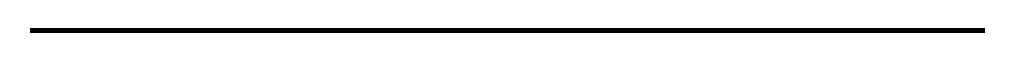
\begin{tikzpicture}
            \draw[line width=2pt] (0,0) -- (\textwidth,0);
        \end{tikzpicture}
        \\[0.5em]
        % Thin decorative line
        \begin{tikzpicture}
            \draw[line width=0.5pt] (0,0) -- (\textwidth,0);
        \end{tikzpicture}
        \\[2.5em]
        % Main title
        {\fontsize{22pt}{26pt}\selectfont\bfseries #1}\\[1.2em]
        % Appendix label
        {\fontsize{16pt}{20pt}\selectfont\bfseries Appendix}\\[2.5em]
        % Bottom lines
        \begin{tikzpicture}
            \draw[line width=0.5pt] (0,0) -- (\textwidth,0);
        \end{tikzpicture}
        \\[0.5em]
        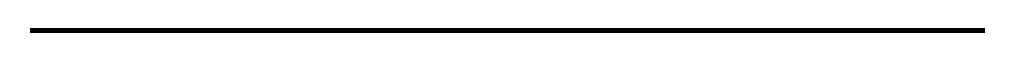
\begin{tikzpicture}
            \draw[line width=2pt] (0,0) -- (\textwidth,0);
        \end{tikzpicture}
    \end{center}
    \vspace{2cm}
}
% Usage: Replace "Your Paper Title" with your actual title
\FancyAppendixTitle{LeJEPA}



\section{Additional Details on Nonlinear Probing}
\label{sec:additional_nonlinear}



\subsection{kNN Probing}


To allow for more flexible evaluation of the pretrained encoder $f_{\vtheta}$, it is standard to work with a $k$-NN prober \citep{taunk2019brief}, both for regression and classification. We rely on the radial $k$-NN variation that leverages a sample-dependent $k$--improving performance for non uniform distributions of samples \citep{sun2010adaptive,zhang2017efficient,abu2019effects}. 


We denote the underlying embedding density as $p_{z}\in C^3$ with derivatives of order up to $3$ bounded, and finite Fisher information and covariance. This regularity condition is fulfilled by current encoders. The {\em unknown} labels come from the target function $\eta:\R^K\to\R$, assumed $C^2$. We handle classification tasks by setting $\eta(\vz)=\mathbb{P}(Y=1\mid \vz)$. The training consists of the $N$ embeddings along with their training labels $\{(\vz_n,\eta(\vz_n))\}_{n=1}^{N}$, where we will denote $\vy_{n}\triangleq \eta(\vz_n)$. The prediction for a query vector $\vq$ is formed as
\begin{align}
\widehat{\vy}(\vq)
:=
\frac{1}{\vy(\vq)}\sum_{n:\norm{\vz_{n}-\vq}\le r_0}\vy_n,\tag{kNN}\label{eq:kNN}
\end{align}
with $\vy(\vq)\triangleq\#\{n:\norm{\vz_{n}-\vq}\le r_0\}$ counting the number of samples within a $r$-radius ball around $\vq$. The radius $r$ controls how many neighbors predictions are averaged to form the query's prediction. As per the linear probing's \cref{thm:linear_probe_bias}, we can characterize the bias of the estimator \cref{eq:kNN} at a particular query point, as formalized below.




\begin{lemma}[label={thm:knn_bias}]{k-NN Pointwise Bias}{}
The \eqref{eq:kNN} estimator has bias at query $\vq$ given by
\begin{multline*}
    \mathrm{Bias}(\vq)=
\frac{r_0^2}{d+2}\Big(\grad\eta(\vq)^\top\grad\log p_{z}(\vq)+\tfrac{1}{2}\Delta\eta(\vz)\Big)\\+o(r_0^2),
\end{multline*}
where the remainder $o(r_0^2)$ is uniform in $\vq$. (Proof in \cref{proof:knn_bias}.)
\end{lemma}


To obtain the integrated bias, i.e., over the distribution of query points, we consider the following two properties. First, the distribution of query points follow the training distribution, i.e., $\vq \sim p_{z}$, second, target function $\eta$ has gradient which is mean-zero and isotropic with $\E\big[\grad\eta(\vz)\grad\eta(\vz)^\top\big]=\tau_g^2I_d$ with $\tau_g^2\in(0,\infty)$
uniformly in $\vz$. We also have any finite scalar-constraint on the covariance of the embeddings such as $\Tr(\Sigma)=c$ or $\|\Sigma\|_F=c$ for a finite constant $c$.



\begin{theorem}[label={thm:knn_optimal}]{k-NN isotropic Gaussian Optimality}{}
The integrated squared bias of \eqref{eq:kNN} satisfies
\[
\E_{\vz}\big[\mathrm{Bias}(\vz)^2\big]
=
\frac{r_0^4}{(K+2)^2}\tau_g^2J(p)\\+O(r_0^4),
\]
and the isotropic Gaussian  is the unique minimizer of the integrated square bias. (Proof in \cref{proof:knn_optimal}.)
\end{theorem}

As a result, we now have a unique minimizer for the optimal embedding density for both the linear and k-NN probes.














\subsection{Kernel Probing}

As an alternative to \eqref{eq:kNN}, it is also common to leverage kernel methods, which we consider in this section.


Consider a kernel $K:\mathbb{R}^K\to\mathbb{R}$ with the following standard properties
\begin{align}
    &\int_{\mathbb{R}^d} K(u)du=1,\tag{normalized}\\
    &\int_{\mathbb{R}^d} uK(u)du=0,\tag{symmetric}\\
    &\int_{\mathbb{R}^d} u u^\top K(u)du=\mu_2(K)I_d,\tag{isotropic}\\
    &R(K)\triangleq\int_{\mathbb{R}^d} K(u)^2du<\infty,\tag{finite roughness}
\end{align}
for some $\mu_2(K)\in(0,\infty)$, some bandwidth $h>0$ and denoting $K_h(t)\triangleq h^{-d}K(t/h)$, we remind the reader that the Nadaraya-Watson estimator, introduced in \citet{nadaraya1964estimating,watson1964smooth}, at a query $\vq\in\mathbb{R}^d$ is
\begin{align}
\widehat \vy(\vq)\triangleq \frac{\sum_{n=1}^N K_h(\vq-\vx_n)\vy_n}{\sum_{n=1}^N K_h(\vq-\vx_n)}.\tag{NW}\label{eq:NW}
\end{align}
Similarly to \eqref{eq:kNN}, we will see that the performance of \eqref{eq:NW} depends crucially on the distribution of the training points. We have access to our dataset of inputs from $p_z$ and for each sample $\vz_n$ the corresponding target is given from $\eta(\vz_n)=\mathbb{E}[Y_n\mid \vz_n]$. We also denote the corresponding conditional variance of the target function at that point as $v(x)=\mathrm{Var}(Y_i\mid X_i=x)$. We follow the regularity conditions of the k-NN probing derivations and additionally assume that $p$ has sufficiently light tails so that for each coordinate $j$, $\lim_{\|x\|\to\infty} p(x)=0$ and $\lim_{\|x\|\to\infty} x_jp(x)=0$. We first derive the pointwise bias and variance for $\widehat \vy(\vq)$.


\begin{lemma}[label={thm:kernel_bias}]{Kernel Bias and Variance}{}
For any fixed $\vq\in\mathbb{R}^d$ with $p(\vq)>0$, as $h\to 0$ and $n h^d\to\infty$,
\begin{align*}
\mathrm{Bias}\big[\widehat \vy(\vq)\big]
&=\frac{h^2\mu_2(K)}{2}\Big(\Delta \vy(\vq)+2\nabla \vy(\vq)^\top \nabla\log p(\vq)\Big)+o(h^2),\\
\mathrm{Var}\big[\widehat \vy(\vq)\big]
&=\frac{R(K)}{n h^d}\frac{v(\vq)}{p(\vq)}+o\big((n h^d)^{-1}\big).
\end{align*}
The $o(\cdot)$ terms are uniform over compact sets where $p$ is bounded away from zero.
(Proof in \cref{proof:kernel_bias}.)
\end{lemma}



We now show that, under a fixed mean and total-covariance constraint on $p_z$, the isotropic Gaussian distribution uniquely minimizes the bias and variance of the kernel regression estimator at any test point. We restrict the smoothness class of the target function using 
\begin{multline*}
    \mathcal{M}(L,B)\triangleq\Big\{m\in C^2(\mathbb{R}^d):\|\nabla \vy(\vq)\|\le L,\\|\Delta \vy(\vq)|\le B, \forall  \vq\in\mathbb{R}^d\Big\},
\end{multline*}
allowing us to formalize below the worst case integrated bias and the optimal density for $z$.



\begin{theorem}[label={thm:kernel_optimal}]{Kernel isotropic Gaussian Optimality}{thm:kernel_optimal}
The integrated squared bias of \eqref{eq:NW} satisfies
\begin{multline*}
\sup_{m\in\mathcal{M}(L,B)}\mathbb{E}_{z}\left[\mathrm{Bias}\big[\widehat \vy(\vz)\big]\right]
\le \Big(\frac{h^2\mu_2(K)}{2}\Big)^2 \Big(2 B^2 + 8 L^2J(p)\Big)+o(h^4),
\end{multline*}
and the integrated variance is independent of $p$. 
Among all densities $p$ on $\mathbb{R}^d$ with total-variance constrained, e.g., $\Tr(\Sigma)=c$, the isotropic Gaussian is the unique minimizer. (Proof in \cref{proof:kernel_optimal}.)
\end{theorem}



\section{Proofs}





\subsection{Proof of \cref{thm:linear_probe_bias}}
\label{proof:linear_probe_bias}


\begin{proof}
Our proof follows standard derivations when it comes to studying the bias of an estimator. Let's consider the ridge regression problem (Tikhonov regularized least squares estimator) with close form estimator
\begin{equation}
\hat{\boldsymbol{\beta}} = (\mathbf{X}^T \mathbf{X} + \lambda_{\rm wd} \mathbf{I})^{-1} \mathbf{X}^T \mathbf{Y}.
\end{equation}
The labels are formed from the ground truth parameter $\beta_{\rm true}$ with centered error, as per $\mathbf{Y} = \mathbf{X}\boldsymbol{\beta}_{\text{true}} + \boldsymbol{\varepsilon}$ where $\mathbb{E}[\boldsymbol{\varepsilon}] = \mathbf{0}$.
We can now look at the bias of our estimator given by
\begin{align*}
\text{Bias}(\hat{\boldsymbol{\beta}}) &= \mathbb{E}[\hat{\boldsymbol{\beta}}] - \boldsymbol{\beta}_{\text{true}} \\
&=(\mathbf{X}^T \mathbf{X} + \lambda_{\rm wd} \mathbf{I})^{-1} \mathbf{X}^T \mathbf{X}\boldsymbol{\beta}_{\text{true}}-\boldsymbol{\beta}_{\text{true}}\\
&= -\lambda_{\rm wd}(\mathbf{X}^T \mathbf{X} + \lambda_{\rm wd} \mathbf{I})^{-1} \boldsymbol{\beta}_{\text{true}}\\
&= -\lambda_{\rm wd} \mathbf{Q}(\boldsymbol{\Lambda} + \lambda \mathbf{I})^{-1}\mathbf{Q}^T \boldsymbol{\beta}_{\text{true}}
\end{align*}
We will now compare that bias when $\mX$ has isotropic and anisotropic covariance with same total variance:
\begin{equation}
\frac{\lambda_1 + \lambda_2 + \cdots + \lambda_p}{p} = \bar{\lambda}.
\end{equation}
For any anisotropic covariance matrix of $\mX$, denote by $\vq_1$ the eigenvector with smallest eigenvalue, and let's denote by $\kappa>0$ a positive constant. We now define
\begin{equation}
\boldsymbol{\beta}_{\text{true}} = \kappa \cdot \mathbf{q}_p,
\end{equation}
leading to
\begin{align*}
\|\text{Bias}(\hat{\boldsymbol{\beta}})\|_{\text{isotropic}} = \frac{\lambda_{\rm wd}}{\bar{\lambda} + \lambda_{\rm wd}} \|\boldsymbol{\beta}_{\text{true}}\|,\\
\|\text{Bias}(\hat{\boldsymbol{\beta}})\|_{\text{non-isotropic}} = \frac{\lambda_{\rm wd}}{\lambda_p + \lambda_{\rm wd}} \|\boldsymbol{\beta}_{\text{true}}\|
\end{align*}
Since $\lambda_p < \bar{\lambda}$ (strict inequality when not isotropic):
\begin{equation*}
\frac{\lambda_{\rm wd}}{\lambda_p + \lambda_{\rm wd}} > \frac{\lambda_{\rm wd}}{\bar{\lambda} + \lambda_{\rm wd}}
\end{equation*}
we obtain that
\begin{equation*}
\|\text{Bias}(\hat{\boldsymbol{\beta}})\|_{\text{non-isotropic}} > \|\text{Bias}(\hat{\boldsymbol{\beta}})\|_{\text{isotropic}}
\end{equation*}


As a result, whenever the covariance matrix of $\mX$ is anisotropic, there will be downstream tasks for which the estimator bias is increased compared to having isotropic covariance matrix.
Anisotropic covariance structure thus amplifies regularization bias when the true parameter vector aligns unfavorably with the data's covariance structure.
\end{proof}






\subsection{Proof of \cref{thm:linear_probe_variance}}
\label{proof:linear_probe_variance}
\begin{proof}
We use the same formula as in \cref{proof:linear_probe_bias} with $\lambda_{\rm wd}=0$. We first see that the estimator is unbiased. We will now leverage that result to compute the covariance matrix of the estimator 
\begin{align*}
\text{Var}(\hat{\boldsymbol{\beta}}|\mathbf{X}) &= \mathbb{E}[(\hat{\boldsymbol{\beta}} - \boldsymbol{\beta})(\hat{\boldsymbol{\beta}} - \boldsymbol{\beta})^T|\mathbf{X}]\\
&= \mathbb{E}[(\mathbf{X}^T\mathbf{X})^{-1}\mathbf{X}^T\boldsymbol{\varepsilon}\boldsymbol{\varepsilon}^T\mathbf{X}(\mathbf{X}^T\mathbf{X})^{-1}|\mathbf{X}]\\
&= (\mathbf{X}^T\mathbf{X})^{-1}\mathbf{X}^T\mathbb{E}[\boldsymbol{\varepsilon}\boldsymbol{\varepsilon}^T|\mathbf{X}]\mathbf{X}(\mathbf{X}^T\mathbf{X})^{-1}\\
&= (\mathbf{X}^T\mathbf{X})^{-1}\mathbf{X}^T(\sigma^2\mathbf{I}_n)\mathbf{X}(\mathbf{X}^T\mathbf{X})^{-1}\\
&= \sigma^2(\mathbf{X}^T\mathbf{X})^{-1}
\end{align*}
leading to the total variance
$$\text{tr}(\text{Var}(\hat{\boldsymbol{\beta}})) = \sigma^2\text{tr}(\mathbf{G}^{-1})=\sigma^2 \sum_{j=1}^p \frac{1}{\lambda_j}$$
where we used the eigendecomposition:
$$\mathbf{G} = \mathbf{Q}\boldsymbol{\Lambda}\mathbf{Q}^T$$



The function $f(x) = \frac{1}{x}$ is strictly convex on $(0, \infty)$ allowing us to leverage Jensen's Inequality:
\begin{align*}
    \frac{1}{K}\sum_{k=1}^K \frac{1}{\lambda_k} > \frac{1}{\frac{1}{K}\sum_{j=1}^K \lambda_k}\\
    \iff \frac{1}{K}\sum_{k=1}^K \frac{1}{\lambda_k} > \frac{1}{K}\sum_{k=1}^{K}\frac{1}{\frac{1}{K}\sum_{j=1}^K \lambda_k}\\
    \iff \sum_{k=1}^K \frac{1}{\lambda_k} > \sum_{k=1}^{K}\frac{1}{\frac{1}{K}\sum_{j=1}^K \lambda_k}\\
    \iff \text{tr}(\text{Var}(\hat{\boldsymbol{\beta}}))_{\text{aniso}} > \text{tr}(\text{Var}(\hat{\boldsymbol{\beta}}))_{\text{iso}}
\end{align*}
The inequality is strict whenever the eigenvalues $\{\lambda_j\}_{j=1}^p$ are not all equal.
\end{proof}











% \subsection*{Appendix: PPP justification for the surrogate ball-average law}
% We sketch why $\E[\widehat{\eta}(x)]$ equals the normalized ball average of $\eta$ weighted by $p$ to second order in $r_0$ under the inhomogeneous PPP with intensity $\lambda(y)=N p(y)$.
% Let $M_x$ be the number of PPP points in $\Ball(x,r_0)$. Then $M_x\sim\mathrm{Poisson}(\mu_x)$ with
% \[
% \mu_x=\int_{\Ball(x,r_0)} \lambda(y)dy
% = N\int_{\Ball(0,r_0)} p(x+u)du
% = N\Big(\vol r_0^dp(x)+\frac{\vol r_0^{d+2}}{2(d+2)}\tr(\Hess p(x))+O(r_0^{d+3})\Big).
% \]
% Conditional on $M_x=m\ge 1$, the $m$ points are i.i.d. with law proportional to $p(x+z)\1\{\norm{z}\le r_0\}$ on $\Ball(0,r_0)$. Thus
% \[
% \E\big[\widehat{\eta}(x)\mid M_x=m\big]
% =\frac{\int_{\Ball(0,r_0)} \eta(x+z)p(x+z)dz}{\int_{\Ball(0,r_0)} p(x+z)dz}.
% \]
% Averaging over $M_x$ leaves the same ratio, because the conditional expectation does not depend on $m$. Therefore
% \[
% \E\big[\widehat{\eta}(x)\big]
% =\frac{\int_{\Ball(0,r_0)} \eta(x+z)p(x+z)dz}{\int_{\Ball(0,r_0)} p(x+z)dz},
% \]
% which is the surrogate used.







% \subsection*{A. Inhomogeneous Poisson point process (PPP) preliminaries}
% Let $\Pi$ be an inhomogeneous Poisson point process on $\mathbb{R}^d$ with locally integrable \emph{intensity} (a.k.a. mean measure density) $\lambda:\mathbb{R}^d\to [0,\infty)$. For any Borel set $A\subset\mathbb{R}^d$,
% \[
% M(A):=\#\big(\Pi\cap A\big)\sim \mathrm{Poisson}\Big(\Lambda(A)\Big),
% \quad
% \Lambda(A):=\int_A \lambda(y)dy,
% \]
% and for disjoint sets $A_1,\dots,A_m$, the counts $M(A_1),\dots,M(A_m)$ are independent. A key conditional law (Kingman, PPP theory) is:
% \begin{lemma}[label={lem:PPP_conditional}]{Special case: Recovery of VCReg}{}
% Fix a bounded Borel set $A$ with $\Lambda(A)>0$. Conditional on $M(A)=m\ge 1$, the $m$ points of $\Pi$ that fall in $A$ are i.i.d. with density
% \[
% q_A(y)
% \;:=\;
% \frac{\lambda(y)\mathbf{1}\{y\in A\}}{\Lambda(A)}\quad \text{on }A.
% \]
% \end{lemma}
% We shall take $\lambda(y)=Np(y)$, where $p$ is the design density of the i.i.d. sample $\{X_i\}_{i=1}^N$; the PPP serves as a standard asymptotic surrogate for the empirical cloud. All statements below can be interpreted either under this PPP directly or (via Poissonization) as approximations for i.i.d. sampling with matching first two moments and the same local calculations.
% \subsection*{B. Equalized-radius scheme and choice of $r_0(N)$, $k(x)$}
% Fix a query location $x\in\mathbb{R}^d$ and a \emph{radius} $r>0$. Let
% \[
% B(x,r):=\{y:\|y-x\|\le r\},\qquad M_x(r):=\#\big(\Pi\cap B(x,r)\big).
% \]
% Under $\lambda(y)=N p(y)$,
% \[
% M_x(r)\sim \mathrm{Poisson}\Big(\mu_x(r)\Big),
% \qquad
% \mu_x(r):=\int_{B(x,r)} N p(y)dy = N \int_{B(0,r)} p(x+u)du.
% \]
% A second-order Taylor expansion yields, uniformly for small $r$,
% \begin{equation}
% \label{eq:mu_expansion}
% \mu_x(r)
% = N\Big(
% v_dr^dp(x)
% + \frac{v_dr^{d+2}}{2(d+2)}\mathrm{tr}(H p(x))
% + O(r^{d+3})
% \Big),
% \end{equation}
% where $v_d$ is the unit-ball volume and $H p$ denotes the Hessian of $p$.
% The \emph{equalized-radius} design sets a deterministic radius $r_0=r_0(N)\downarrow 0$ (as $N\to\infty$) and uses all points in $B(x,r_0)$ to estimate $\eta(x)$; thus the neighbor count is random:
% \[
% M_x := M_x(r_0)\sim \mathrm{Poisson}\big(\mu_x(r_0)\big).
% \]
% To make the \emph{expected} number of neighbors essentially independent of $x$ up to second order, we choose $r_0$ via the scale relation
% \begin{equation}
% \label{eq:r0_kappa}
% v_dr_0(N)^d \ :=:\ \kappa_N \ \downarrow 0,
% \qquad
% \text{with}\quad N\kappa_N \to \infty,
% \end{equation}
% so that the leading term in \eqref{eq:mu_expansion} is $Nv_dr_0^dp(x) = N\kappa_Np(x)$ while the second-order correction is $O\big(Nr_0^{d+2}\big) = O\big(N\kappa_N^{1+2/d}\big)$. Under mild regularity, this correction is negligible relative to the leading term provided
% \[
% N\kappa_N \to \infty
% \quad\text{and}\quad
% \kappa_N^{2/d} \to 0,
% \]
% which both hold if $r_0(N)\downarrow 0$ and $N r_0(N)^d \to \infty$.
% For reference, one can also parameterize by a \emph{variable-$k$} rule:
% \[
% k(x) \ :=\ \kappa_NNp(x).
% \]
% In a locally homogeneous PPP ($p$ nearly constant at scale $r_0$), the $k(x)$-th nearest-neighbor distance $R_{k(x)}(x)$ concentrates around the deterministic $r_0=(\kappa_N/v_d)^{1/d}$. Indeed, in a homogeneous PPP with intensity $\lambda_0$, the pdf of $R_k$ is
% \[
% f_{R_k}(r)
% = \frac{d\lambda_0v_dr^{d-1}}{(k-1)!}
% \big(\lambda_0v_dr^d\big)^{k-1}e^{-\lambda_0v_dr^d},
% \]
% so $\lambda_0 v_d r_k^d\approx k$ (mode/mean), whence $r_k\approx (k/(\lambda_0 v_d))^{1/d}$. Taking $\lambda_0=N p(x)$ and $k(x)=\kappa_N N p(x)$ yields $r_k(x)\approx (\kappa_N/v_d)^{1/d}=r_0$. Moreover,
% \[
% \frac{\mathrm{Var}(R_k^d)}{(\E R_k^d)^2}=\frac{1}{k}\qquad\Rightarrow\qquad
% \frac{R_k - r_0}{r_0} = O_{\mathbb{P}}\Big(\frac{1}{\sqrt{k}}\Big)
% = O_{\mathbb{P}}\Big((N\kappa_Np(x))^{-1/2}\Big),
% \]
% so $R_{k(x)}(x)$ concentrates around $r_0$ uniformly on regions with $p(x)\ge c>0$ whenever $N\kappa_N\to\infty$.
% \subsection*{C. Exact formula for $\mathbb{E}[\widehat{\eta}(x)]$ under PPP}
% Consider the local-constant \emph{ball-average} estimator at radius $r_0$:
% \[
% \widehat{\eta}(x)
% \;:=\;
% \begin{cases}
% \displaystyle\frac{1}{M_x}\sum_{Y\in \Pi\cap B(x,r_0)} \eta(Y), & M_x\ge 1,\\[1.2ex]
% 0, & M_x=0.
% \end{cases}
% \]
% (Any deterministic fallback for $M_x=0$ is acceptable; see below.)
% \begin{proposition}[label={prop:exact_ratio}]{Special case: Recovery of VCReg}{}
% \label{prop:exact_ratio}
% With $\lambda(y)=N p(y)$ and $M_x:=M_x(r_0)$, we have
% \[
% \mathbb{E}\big[\widehat{\eta}(x)\big| M_x=m\big]
% \;=\;
% \frac{\int_{B(0,r_0)} \eta(x+z)p(x+z)dz}{\int_{B(0,r_0)} p(x+z)dz}
% \qquad \text{for every }m\ge 1.
% \]
% Consequently,
% \[
% \mathbb{E}\big[\widehat{\eta}(x)\big| M_x\ge 1\big]
% \;=\;
% \frac{\int_{B(0,r_0)} \eta(x+z)p(x+z)dz}{\int_{B(0,r_0)} p(x+z)dz}.
% \]
% \end{proposition}
% \begin{proof}
% By Lemma~\ref{lem:PPP_conditional} with $A=B(x,r_0)$, conditional on $M_x=m$, the $m$ points in $B(x,r_0)$ are i.i.d. with density proportional to $\lambda(y)=N p(y)$ on $B(x,r_0)$; equivalently, with density
% \[
% q_{x,r_0}(y) \;=\; \frac{p(y)\mathbf{1}\{\|y-x\|\le r_0\}}{\int_{B(x,r_0)} p(u)du}.
% \]
% Therefore,
% \[
% \mathbb{E}\left[\frac{1}{m}\sum_{j=1}^m \eta(Y_j)\Big|M_x=m\right]
% = \int_{B(x,r_0)} \eta(y)q_{x,r_0}(y)dy
% = \frac{\int_{B(x,r_0)} \eta(y)p(y)dy}{\int_{B(x,r_0)} p(y)dy}.
% \]
% Changing variables $y=x+z$ gives the stated ratio. Since the right-hand side is independent of $m$, the same holds conditional on $M_x\ge 1$ by averaging over $m\ge 1$.
% \end{proof}
% \begin{corollary}[label={cor:uncond}]{Special case: Recovery of VCReg}{}
% Let $\mu_x:=\mu_x(r_0)=\int_{B(x,r_0)} N p(y)dy$. Then
% \[
% \mathbb{E}\big[\widehat{\eta}(x)\big]
% = \mathbb{P}(M_x\ge 1)\cdot
% \frac{\int_{B(0,r_0)} \eta(x+z)p(x+z)dz}{\int_{B(0,r_0)} p(x+z)dz}.
% \]
% Moreover, $\mathbb{P}(M_x=0)=e^{-\mu_x}$. Hence, if $N r_0(N)^d\inf_{x\in \mathcal{K}} p(x)\to \infty$ on a compact $\mathcal{K}$, then $\sup_{x\in \mathcal{K}}\big|\mathbb{E}[\widehat{\eta}(x)] - \frac{\int \eta p}{\int p}\big| \le e^{-\mu_x}$ vanishes exponentially fast in $N r_0^d$.
% \end{corollary}
% \begin{proof}
% Condition on $\{M_x=0\}$ and $\{M_x\ge 1\}$ and use Proposition~\ref{prop:exact_ratio}. The Poisson count identity gives $\mathbb{P}(M_x=0)=e^{-\mu_x}$. The uniform bound follows from \eqref{eq:mu_expansion} and the lower bound on $p$ on $\mathcal{K}$.
% \end{proof}



\subsection{Proof of \cref{thm:knn_bias}}
\label{proof:knn_bias}
\begin{proof}

Under PPP, conditional expectations of $\widehat{\eta}(x)$ coincide with the normalized ball average
\[
\E\big[\widehat{\eta}(x)\big]
\;=\;
\frac{\int_{\Ball(0,r_0)} \eta(x+z)p(x+z)dz}{\int_{\Ball(0,r_0)} p(x+z)dz}
\quad\text{to second order in }r_0,
\]
which is the key surrogate used below.
\medskip
\noindent\textbf{Ball integrals.} For computations we use (by symmetry) for any $r>0$:
\[
\int_{\Ball(0,r)} zdz=0,\qquad
\int_{\Ball(0,r)} zz^\top dz=\frac{{\rm Vol}^{d+2}}{d+2}I_d,\qquad
\int_{\Ball(0,r)} \norm{z}^2dz=\frac{d{\rm Vol}^{d+2}}{d+2}.
\]


Fix $x\in\R^d$ and write $z\in\Ball(0,r_0)$ for local displacements. 
Assume $p\in C^3$, $\eta\in C^2$ with bounded derivatives on the region of interest, and expand a second-order Taylor expansion:
\begin{align*}
p(x+z)&=p(x)+\nabla p(x)^\top z+\tfrac12 z^\top H p(x)z + O(\|z\|^3),\\
\eta(x+z)&=\eta(x)+\nabla\eta(x)^\top z+\tfrac12 z^\top H\eta(x)z + O(\|z\|^3),
\end{align*}
with remainders satisfying $|R_\eta(x;z)|\le C_\eta\norm{z}^3$ and $|R_p(x;z)|\le C_p\norm{z}^3$ uniformly for $\norm{z}\le r_0$. Using the ball identities
$\int_{B(0,r)} zdz=0$ and $\int_{B(0,r)} zz^\top dz=\frac{v_d r^{d+2}}{d+2}I_d$ and collecting terms up to order $r_0^{d+2}$, we simplify the denominator as
\begin{align*}
    \mathcal{D}(x)&\triangleq\int_{\Ball(0,r_0)} p(x+z)dz\\
    &= \int_{\Ball(0,r_0)} \Big[p(x) + \grad p(x)^\top z + \tfrac{1}{2}z^\top \Hess p(x)z + R_p(x;z)\Big]dz\\
    &= {\rm Vol}_0^dp(x)\;+\;\frac{{\rm Vol}_0^{d+2}}{2(d+2)}\tr\big(\Hess p(x)\big)\;+\;O(r_0^{d+3}),
\end{align*}
since $\int zdz=0$ and $\int z^\top \Hess pzdz=\tr(\Hess p)\frac{\vol r_0^{d+2}}{d+2}$ and the denominator as
\begin{align*}
\mathcal{N}(x)&\triangleq \int_{\Ball(0,r_0)} \eta(x+z)p(x+z)dz\\
    &= \int \Big[\eta(x)+\grad\eta(x)^\top z+\tfrac{1}{2}z^\top \Hess\eta(x)z\Big]
\Big[p(x)+\grad p(x)^\top z+\tfrac{1}{2}z^\top \Hess p(x)z\Big]dz+O(r_0^{d+3})\\
&= \eta(x)p(x)\vol r_0^d+\eta(x)\frac{\vol r_0^{d+2}}{2(d+2)}\tr\big(\Hess p(x)\big)+\frac{\vol r_0^{d+2}}{d+2}\grad\eta(x)\cdot\grad p(x)+ \frac{\vol r_0^{d+2}}{2(d+2)}p(x)\tr\big(\Hess\eta(x)\big)
+O(r_0^{d+3}).
\end{align*}


% Define the numerator and denominator
% \[
% \mathcal{N}(x):=\int_{\Ball(0,r_0)} \eta(x+z)p(x+z)dz,\qquad
% \mathcal{D}(x):=\int_{\Ball(0,r_0)} p(x+z)dz.
% \]
% We expand both to order $r_0^{d+2}$.
% \emph{Denominator.} Using symmetry:
% \begin{align*}
% \mathcal{D}(x)
% &= \int_{\Ball(0,r_0)} \Big[p(x) + \grad p(x)^\top z + \tfrac{1}{2}z^\top \Hess p(x)z + R_p(x;z)\Big]dz\\
% &= {\rm Vol}_0^dp(x)\;+\;\frac{{\rm Vol}_0^{d+2}}{2(d+2)}\tr\big(\Hess p(x)\big)\;+\;O(r_0^{d+3}),
% \end{align*}
% since $\int zdz=0$ and $\int z^\top \Hess pzdz=\tr(\Hess p)\frac{\vol r_0^{d+2}}{d+2}$.
% \emph{Numerator.} Expanding the product and integrating term-by-term:
% \begin{align*}
% \mathcal{N}(x)
% &= \int \Big[\eta(x)+\grad\eta(x)^\top z+\tfrac{1}{2}z^\top \Hess\eta(x)z\Big]
% \Big[p(x)+\grad p(x)^\top z+\tfrac{1}{2}z^\top \Hess p(x)z\Big]dz\;+\;O(r_0^{d+3})\\
% &= \eta(x)p(x)\vol r_0^d\\
% &\quad+\ \eta(x)\frac{\vol r_0^{d+2}}{2(d+2)}\tr\big(\Hess p(x)\big)\\
% &\quad+\ \frac{\vol r_0^{d+2}}{d+2}\grad\eta(x)\cdot\grad p(x)\\
% &\quad+\ \frac{\vol r_0^{d+2}}{2(d+2)}p(x)\tr\big(\Hess\eta(x)\big)
% \;+\;O(r_0^{d+3}).
% \end{align*}
% Indeed, the $\grad\eta\cdot z$ term paired with $p(x)$ integrates to $0$, while $\int (\grad\eta\cdot z)(\grad p^\top z)dz=\grad\eta^\top\Big(\int zz^\top dz\Big)\grad p=\frac{\vol r_0^{d+2}}{d+2}\grad\eta\cdot\grad p$. 
Cubic terms vanish by symmetry, and quartic terms are $O(r_0^{d+4})$. 
Subtract $\eta(x)\mathcal{D}(x)$ to obtain the bias numerator:
\[
\mathcal{N}(x)-\eta(x)\mathcal{D}(x)
= \frac{v_dr_0^{d+2}}{d+2}\Big(\nabla\eta(x)\cdot\nabla p(x) + \tfrac{1}{2}p(x)\Delta\eta(x)\Big) + O(r_0^{d+3}).
\]
Write $\mathcal{D}(x)=v_d r_0^d p(x)\big(1+\alpha(x)r_0^2+O(r_0^3)\big)$ where $\alpha(x):=\frac{1}{2(d+2)p(x)}\mathrm{tr}(H p(x))$. Then
\begin{align*}
\frac{\mathcal{N}(x)}{\mathcal{D}(x)}-\eta(x)
&= \frac{ \frac{v_d r_0^{d+2}}{d+2}\left(\nabla\eta\cdot\nabla p + \frac{1}{2}p\Delta\eta\right) + O(r_0^{d+3})}{ v_d r_0^d p \left(1+\alpha r_0^2+O(r_0^3)\right)}\\[0.5ex]
&= \frac{r_0^2}{d+2}\left(\frac{\nabla\eta\cdot\nabla p}{p} + \frac{1}{2}\Delta\eta\right)\Big(1-\alpha r_0^2+O(r_0^3)\Big)\ +\ O(r_0^3)\\[0.5ex]
&= \frac{r_0^2}{d+2}\Big(\nabla\eta(x)\cdot\nabla\log p(x) + \tfrac{1}{2}\Delta\eta(x)\Big)\ +\ o(r_0^2),
\end{align*}
uniformly on $\mathcal{K}$. This gives the bias formula
\[
\mathbb{E}\big[\widehat{\eta}(x)\big]-\eta(x)
=
\frac{r_0^2}{d+2}\Big(\nabla\eta(x)\cdot\nabla\log p(x) + \tfrac{1}{2}\Delta\eta(x)\Big)\ +\ o(r_0^2),
\]


% Subtracting $\eta(x)\mathcal{D}(x)$ to $\mathcal{N}$ cancels the common terms and yields
% \[
% \mathcal{N}(x)-\eta(x)\mathcal{D}(x)
% = \frac{v_d r_0^{d+2}}{d+2}\Big(\nabla\eta(x)\cdot\nabla p(x) + \tfrac12 p(x)\Delta\eta(x)\Big) + O(r_0^{d+3}).
% \]
% Dividing by $\mathcal{D}(x)$ and using the expansion
% $\mathcal{D}(x)^{-1} = (v_d r_0^d p(x))^{-1}\big(1+O(r_0^2)\big)$, we get
% \begin{align*}
% \frac{\mathcal{N}(x)}{\mathcal{D}(x)} - \eta(x)
% &=\frac{r_0^2}{d+2}\Big(\frac{\grad\eta(x)\cdot\grad p(x)}{p(x)}+\tfrac{1}{2}\Delta\eta(x)\Big)\;+\;o(r_0^2)\\
% &= \frac{r_0^2}{d+2}\Big(\nabla\eta(x)\cdot\nabla \log p(x) + \tfrac12 \Delta\eta(x)\Big) + o(r_0^2),    
% \end{align*}
completing the proof.
\end{proof}


% Assume $p\in C^3$, $\eta\in C^2$ with bounded derivatives on the region of interest, and expand:
% \begin{align*}
% p(x+z)&=p(x)+\nabla p(x)^\top z+\tfrac12 z^\top H p(x)z + O(\|z\|^3),\\
% \eta(x+z)&=\eta(x)+\nabla\eta(x)^\top z+\tfrac12 z^\top H\eta(x)z + O(\|z\|^3).
% \end{align*}
% Using the ball identities
% $\int_{B(0,r)} zdz=0$ and $\int_{B(0,r)} zz^\top dz=\frac{v_d r^{d+2}}{d+2}I_d$ and collecting terms up to order $r_0^{d+2}$, one obtains
% \begin{align*}
% \mathcal{D}(x) &= v_d r_0^dp(x) + \frac{v_d r_0^{d+2}}{2(d+2)}\mathrm{tr}(H p(x)) + O(r_0^{d+3}),\\
% \mathcal{N}(x)
% &= v_d r_0^d\eta(x)p(x)
% + \frac{v_d r_0^{d+2}}{d+2}\nabla\eta(x)\cdot\nabla p(x)
% + \frac{v_d r_0^{d+2}}{2(d+2)}\Big(\eta(x)\mathrm{tr}(H p(x)) + p(x)\mathrm{tr}(H\eta(x))\Big)
% + O(r_0^{d+3}).
% \end{align*}

% \subsection*{E. Concentration of the $k(x)$-NN radius around $r_0$}
% For completeness, we record a simple concentration argument in the homogeneous proxy (valid locally for smooth $p$). Fix $x$ and let $\lambda_0:=N p(x)$. In a homogeneous PPP of intensity $\lambda_0$, $M_x(r)\sim\mathrm{Poisson}(\lambda_0 v_d r^d)$. For $\epsilon\in(0,1)$,
% \[
% \mathbb{P}\left(M_x\big(r_0(1+\epsilon)\big) < k(x)\right)
% \;=\;
% \mathbb{P}\left(\mathrm{Poisson}\big(\lambda_0 v_d r_0^d (1+\epsilon)^d\big) < \lambda_0 v_d r_0^d\right)
% \;\le\; \exp\Big(-c_+k(x)\epsilon^2\Big),
% \]
% and similarly
% \[
% \mathbb{P}\left(M_x\big(r_0(1-\epsilon)\big) > k(x)\right)
% \;\le\; \exp\Big(-c_-k(x)\epsilon^2\Big),
% \]
% by standard Poisson Chernoff bounds, with $c_\pm=c_\pm(d)>0$. Since $R_{k(x)}(x)$ is the inverse of the nondecreasing mapping $r\mapsto M_x(r)$, we conclude
% \[
% \mathbb{P}\left(\big|R_{k(x)}(x) - r_0\big| > \epsilon r_0\right)
% \;\le\; 2\exp\Big(-ck(x)\epsilon^2\Big),
% \]
% for some $c=c(d)>0$. With $k(x)=\kappa_N N p(x)$ and $N\kappa_N\to\infty$, this gives exponential concentration uniformly on compact sets where $p(x)\ge c_0>0$.
% \subsection*{F. Scaling for consistency and relation to the variable-$k$ scheme}
% To ensure consistency of local-constant estimators, one typically requires (i) the localization radius to shrink, and (ii) the number of neighbors to grow: as $N\to\infty$,
% \[
% r_0(N)\downarrow 0,
% \qquad
% \mu_x(r_0(N))=N\int_{B(x,r_0(N))}p(y)dy \to \infty
% \quad\text{(uniformly on compact sets)}.
% \]
% Under \eqref{eq:r0_kappa}, these are equivalent to
% \[
% \kappa_N=v_d r_0(N)^d \to 0
% \quad\text{and}\quad
% N\kappa_N \to \infty,
% \]
% and the equalized variable-$k$ rule is $k(x)=\kappa_N N p(x)\to\infty$ at all $x$ with $p(x)>0$, while the \emph{effective} radius $r_0(N)=(\kappa_N/v_d)^{1/d}\downarrow 0$ is independent of $x$. This is the regime under which the second-order bias expansion and the Fisher-information design principle hold uniformly on compact subsets of $\{x:p(x)>0\}$.


% This appendix provides step-by-step derivations of the expected bias of the equalized-radius local-constant $k$-NN estimator, under the inhomogeneous PPP surrogate with intensity $\lambda(y)=N p(y)$. We present two complementary derivations:
% (i) a \emph{ratio-of-integrals} expansion directly for $\mathbb{E}[\widehat{\eta}(x)]$; and
% (ii) a \emph{moment-based} expansion via $\mathbb{E}[Z]$ and $\mathbb{E}[ZZ^\top]$, with $Z:=X_{(1)}(x)-x$ the nearest-neighbor displacement under the equalized-radius scheme.
% Throughout we assume $p\in C^3$ and $\eta\in C^2$ with bounded derivatives (as specified precisely below), and we work uniformly on compact subsets $\mathcal{K}\subset\{x:p(x)>0\}$.
% \subsection*{A. Ratio-of-integrals derivation (ball-average estimator)}
% Fix a query $x\in\mathbb{R}^d$ and a deterministic radius $r_0>0$. Consider the local-constant \emph{ball-average} estimator
% \[
% \widehat{\eta}(x)
% \;:=\;
% \frac{1}{M_x}\sum_{Y\in \Pi\cap B(x,r_0)} \eta(Y)
% \quad\text{if }M_x\ge 1,
% \qquad
% \widehat{\eta}(x):=0\quad\text{if }M_x=0,
% \]
% where $M_x:=\#(\Pi\cap B(x,r_0))$ and $\Pi$ is a PPP with $\lambda(y)=N p(y)$.
% By the conditional i.i.d.\ structure of PPP points inside $B(x,r_0)$ (Lemma~\ref{lem:PPP_conditional}), conditional on $M_x=m\ge 1$ the $m$ points are i.i.d.\ with density
% \[
% q_{x,r_0}(y)=\frac{p(y)\mathbf{1}\{\|y-x\|\le r_0\}}{\int_{B(x,r_0)}p(u)du},
% \]
% and thus
% \[
% \mathbb{E}\big[\widehat{\eta}(x)\big|M_x=m\big]
% =
% \frac{\int_{B(x,r_0)} \eta(y)p(y)dy}{\int_{B(x,r_0)}p(y)dy}.
% \]
% Since the right-hand side is independent of $m$, we have the exact conditional expectation given $M_x\ge 1$:
% \begin{equation}
% \label{eq:ratio_cond}
% \mathbb{E}\big[\widehat{\eta}(x)\big|M_x\ge 1\big]
% =
% \frac{\int_{B(0,r_0)} \eta(x+z)p(x+z)dz}{\int_{B(0,r_0)}p(x+z)dz}.
% \end{equation}
% Unconditionally,
% \begin{align}
% \mathbb{E}[\widehat{\eta}(x)]
% =
% \mathbb{P}(M_x\ge 1)
% \frac{\int_{B(0,r_0)} \eta(x+z)p(x+z)dz}{\int_{B(0,r_0)}p(x+z)dz},
% \end{align}
% and $\mathbb{P}(M_x=0)=\exp\{-\mu_x\}$ with $\mu_x=N\int_{B(0,r_0)}p(x+u)du$. Under the equalization scaling $N r_0^d \inf_{x\in \mathcal{K}} p(x)\to\infty$, $\mathbb{P}(M_x=0)$ is exponentially small uniformly on $\mathcal{K}$, hence negligible. We thus focus on the ratio \eqref{eq:ratio_cond}.
% Define the numerator and denominator
% \[
% \mathcal{N}(x):=\int_{B(0,r_0)} \eta(x+z)p(x+z)dz,
% \qquad
% \mathcal{D}(x):=\int_{B(0,r_0)} p(x+z)dz.
% \]
% We will derive a second-order expansion for the ratio $\mathcal{N}(x)/\mathcal{D}(x)$, and hence the bias $\mathbb{E}[\widehat{\eta}(x)]-\eta(x)$.
% % \paragraph{Assumptions and Taylor expansions.}
% % Assume:
% % - $p\in C^3$ and $\eta\in C^2$ on a neighborhood of $\mathcal{K}$;
% % - There are constants $M_1,M_2,M_3>0$ such that $\sup_{x\in \mathcal{K}} \|\nabla p(x)\|\le M_1$, $\sup_{x\in \mathcal{K}} \|H p(x)\|\le M_2$, and $\sup_{x\in \mathcal{K}} \|D^3 p(x)\|\le M_3$ (operator norms), and similarly for $\eta$ up to order 2.
% % For $\|z\|\le r_0$ and $x\in\mathcal{K}$, expand
% % \begin{align*}
% % p(x+z)&=p(x)+\nabla p(x)^\top z+\tfrac{1}{2} z^\top H p(x)z + R_p(x;z),\\
% % \eta(x+z)&=\eta(x)+\nabla\eta(x)^\top z+\tfrac{1}{2} z^\top H\eta(x)z + R_\eta(x;z),
% % \end{align*}
% % with remainders controlled by Taylor's theorem with integral form:
% % \[
% % |R_p(x;z)|\le \frac{M_3}{6}\|z\|^3,\qquad |R_\eta(x;z)|\le C_\eta\|z\|^3,
% % \]
% % for some $C_\eta>0$ (depending on uniform bounds on $D^3\eta$).
% % \paragraph{Ball integral identities.}
% % We will use:
% % \[
% % \int_{B(0,r)} zdz=0,\quad
% % \int_{B(0,r)} zz^\topdz=\frac{v_dr^{d+2}}{d+2}I_d,\quad
% % \int_{B(0,r)} \|z\|^2dz=\frac{dv_dr^{d+2}}{d+2},
% % \]
% % and the bound $\int_{B(0,r)} \|z\|^3dz = O(r^{d+3})$ with constant depending only on $d$.
% % \paragraph{Denominator expansion.}
% % By symmetry,
% % \begin{align*}
% % \mathcal{D}(x)
% % &= \int_{B(0,r_0)} \Big[p(x) + \nabla p(x)^\top z + \tfrac{1}{2} z^\top H p(x)z + R_p(x;z)\Big]dz\\
% % &= v_dr_0^dp(x)\ +\ \frac{v_dr_0^{d+2}}{2(d+2)}\mathrm{tr}(H p(x))\ +\ O(r_0^{d+3}).
% % \end{align*}
% % \paragraph{Numerator expansion.}
% % Multiplying expansions and integrating term-by-term:
% % \begin{align*}
% % \mathcal{N}(x)
% % &= \int_{B(0,r_0)} \Big[\eta(x)+\nabla\eta(x)^\top z+\tfrac{1}{2} z^\top H\eta(x)z + R_\eta(x;z)\Big]\\
% % &\qquad\qquad\cdot \Big[p(x)+\nabla p(x)^\top z+\tfrac{1}{2} z^\top H p(x)z + R_p(x;z)\Big]dz\\[0.5ex]
% % &= v_dr_0^d\eta(x)p(x)\\
% % &\quad + \frac{v_dr_0^{d+2}}{d+2}\nabla\eta(x)\cdot\nabla p(x)\\
% % &\quad + \frac{v_dr_0^{d+2}}{2(d+2)}\Big[\eta(x)\mathrm{tr}(H p(x)) + p(x)\mathrm{tr}(H\eta(x))\Big]\\
% % &\quad + O(r_0^{d+3}).
% % \end{align*}
% % Here:
% % - The linear terms $\eta(x)\nabla p(x)^\top z$ and $p(x)\nabla\eta(x)^\top z$ integrate to $0$.
% % - The cross term $(\nabla\eta(x)^\top z)(\nabla p(x)^\top z)$ integrates to $\nabla\eta(x)^\top \big(\int zz^\top dz\big)\nabla p(x) = \frac{v_d r_0^{d+2}}{d+2}\nabla\eta(x)\cdot\nabla p(x)$.
% % - The quadratic terms $\tfrac{1}{2}\eta(x)z^\top H p(x)z$ and $\tfrac{1}{2}p(x)z^\top H\eta(x)z$ integrate to the trace forms above.
% % - Remainders $R_\eta, R_p$ contribute $O(r_0^{d+3})$ using the $\|z\|^3$ bound.

% % \subsection*{B. Moment-based derivation via $\mathbb{E}[Z]$ and $\mathbb{E}[ZZ^\top]$}
% % Define the nearest-neighbor displacement $Z:=X_{(1)}(x)-x$. Under the equalized-radius scheme, the law of $Z$ can be approximated (to second order in $r_0$) by the probability measure $\mathbb{Q}_x$ on $B(0,r_0)$ with density
% % \[
% % d\mathbb{Q}_x(z)
% % \;:=\;
% % \frac{p(x+z)}{\int_{B(0,r_0)} p(x+u)du}dz.
% % \]
% % This surrogate captures the leading geometric bias induced by the inhomogeneity of $p$ and the uniform radius; it arises from the PPP calculation that (i) the radius $R:=\|Z\|$ concentrates sharply near $r_0$ (Section~E), and (ii) conditional on $R=r$, the direction $U:=Z/R$ has density proportional to $p(x+rU)$ on the sphere, whence integrating $r$ against the concentrated law yields the ball-weighted density $p(x+z)$ up to $O(r_0^2)$ corrections.
% % We compute the first two moments under $\mathbb{Q}_x$ and then use the Taylor expansion of $\eta$.
% % \paragraph{First moment $\mathbb{E}[Z]$.}
% % Expand $p(x+z)$ as before and integrate:
% % \begin{align*}
% % \int_{B(0,r_0)} zp(x+z)dz
% % &= \int_{B(0,r_0)} z\Big( p(x) + \nabla p(x)^\top z + \tfrac{1}{2}z^\top H p(x)z + O(\|z\|^3)\Big)dz\\
% % &= \int_{B(0,r_0)} z\big(\nabla p(x)^\top z\big)dz \ +\ O(r_0^{d+3})\\
% % &= \frac{v_dr_0^{d+2}}{d+2}\nabla p(x)\ +\ O(r_0^{d+3}).
% % \end{align*}
% % Similarly,
% % \[
% % \int_{B(0,r_0)} p(x+z)dz
% % = v_dr_0^dp(x) + \frac{v_dr_0^{d+2}}{2(d+2)}\mathrm{tr}(H p(x)) + O(r_0^{d+3}).
% % \]
% % Therefore,
% % \begin{align*}
% % \mathbb{E}_{\mathbb{Q}_x}[Z]
% % &= \frac{ \frac{v_dr_0^{d+2}}{d+2}\nabla p(x) + O(r_0^{d+3}) }{ v_dr_0^dp(x)\left(1+\frac{r_0^2}{2(d+2)p(x)}\mathrm{tr}(H p(x)) + O(r_0^3)\right)}\\
% % &= \frac{r_0^2}{d+2}\nabla\log p(x)\ +\ O(r_0^4),
% % \end{align*}
% % uniformly on $\mathcal{K}$.
% % \paragraph{Second moment $\mathbb{E}[ZZ^\top]$.}
% % Compute
% % \begin{align*}
% % \int_{B(0,r_0)} zz^\topp(x+z)dz
% % &= p(x)\int_{B(0,r_0)} zz^\topdz \ +\ O(r_0^{d+4})\\
% % &= \frac{v_dr_0^{d+2}}{d+2}p(x)I_d \ +\ O(r_0^{d+4}).
% % \end{align*}
% % Divide by the same denominator to get
% % \[
% % \mathbb{E}_{\mathbb{Q}_x}[ZZ^\top]
% % = \frac{r_0^2}{d+2}I_d \ +\ O(r_0^4),
% % \]
% % uniformly on $\mathcal{K}$.
% % \paragraph{Bias via Taylor of $\eta$.}
% % With $Z$ as above,
% % \[
% % \eta(x+Z)
% % = \eta(x) + \nabla\eta(x)^\top Z + \tfrac{1}{2}Z^\top H\eta(x)Z + R_\eta(x;Z),
% % \quad
% % |R_\eta(x;Z)|\le C_\eta\|Z\|^3.
% % \]
% % Taking expectation under $\mathbb{Q}_x$ (and hence under the true law up to $O(r_0^2)$ corrections),
% % \begin{align*}
% % \mathbb{E}[\widehat{\eta}(x)] - \eta(x)
% % &= \nabla\eta(x)^\top\mathbb{E}[Z] + \tfrac{1}{2}\mathrm{tr}\big(H\eta(x)\mathbb{E}[ZZ^\top]\big) + \mathbb{E}[R_\eta(x;Z)] + o(r_0^2)\\
% % &= \nabla\eta(x)^\top\left(\frac{r_0^2}{d+2}\nabla\log p(x)\right) + \tfrac{1}{2}\mathrm{tr}\left(H\eta(x)\frac{r_0^2}{d+2}I_d\right) + O(r_0^3) + o(r_0^2)\\
% % &= \frac{r_0^2}{d+2}\Big(\nabla\eta(x)\cdot\nabla\log p(x) + \tfrac{1}{2}\Delta\eta(x)\Big)\ +\ o(r_0^2),
% % \end{align*}
% % uniformly on $\mathcal{K}$. This matches the ratio-of-integrals derivation.
% \subsection*{C. Uniformity, remainder control, and the zero-count event}
% We collect the remainder controls used above and the treatment of the $\{M_x=0\}$ event.
% \paragraph{Remainders.}
% Under the stated $C^3/C^2$ regularity and bounded derivatives, the Taylor remainders satisfy $|R_p(x;z)|\le C_p \|z\|^3$, $|R_\eta(x;z)|\le C_\eta \|z\|^3$. Integrating over the ball yields $O(r_0^{d+3})$ contribution to $\mathcal{N}(x)$ and $O(r_0^{d+3})$ to $\mathcal{D}(x)$. Upon dividing the numerator remainder by $\mathcal{D}(x)\asymp v_d r_0^d p(x)$, the induced error in the ratio is $O(r_0^3)$, which is $o(r_0^2)$ as $r_0\to 0$. The same order arises from multiplying by $(1-\alpha r_0^2 + O(r_0^3))$.
% \paragraph{Zero-count event $\{M_x=0\}$.}
% We have $M_x\sim\mathrm{Poisson}(\mu_x)$ with
% \[
% \mu_x
% = N\int_{B(0,r_0)} p(x+u)du
% = Nv_d r_0^d p(x) + O\big(N r_0^{d+2}\big).
% \]
% Hence $\mathbb{P}(M_x=0)=e^{-\mu_x}$. Under the equalization regime $N r_0^d\inf_{x\in \mathcal{K}}p(x)\to\infty$, we obtain
% \[
% \sup_{x\in \mathcal{K}} \left|
% \mathbb{E}[\widehat{\eta}(x)] - \frac{\int_{B(0,r_0)} \eta(x+z)p(x+z)dz}{\int_{B(0,r_0)} p(x+z)dz}
% \right|
% \ \le\
% \sup_{x\in \mathcal{K}} e^{-\mu_x}
% \ \xrightarrow[N\to\infty]{}\ 0
% \]
% exponentially fast. This justifies ignoring the $\{M_x=0\}$ contribution in the bias expansion.
% \subsection*{D. Choice and scaling of $r_0(N)$ and variable $k(x)$}
% To ensure consistency and the validity of the second-order expansion uniformly on $\mathcal{K}$, one requires
% \[
% r_0(N)\downarrow 0,
% \qquad
% N r_0(N)^d \to \infty,
% \]
% which guarantee (i) localization; and (ii) many points in $B(x,r_0)$ on average. Parameterize $r_0$ by $\kappa_N:=v_d r_0(N)^d\to 0$ with $N\kappa_N\to\infty$. The \emph{variable-$k$} rule $k(x)=\kappa_N N p(x)$ then yields the equalized effective radius
% \[
% r_{k(x)}(x)\approx \Big(\frac{k(x)}{N v_d p(x)}\Big)^{1/d} = \Big(\frac{\kappa_N}{v_d}\Big)^{1/d} = r_0(N),
% \]
% with exponential concentration:
% \[
% \mathbb{P}\left(\big|R_{k(x)}(x)-r_0\big|>\epsilon r_0\right)
% \ \le\
% 2\exp\big(-ck(x)\epsilon^2\big)
% =
% 2\exp\big(-c\kappa_N N p(x)\epsilon^2\big),
% \]
% uniformly on $\mathcal{K}$ where $p(x)\ge c_0>0$.
% \subsection*{E. Summary bias formula}
% Combining the derivations above, uniformly on compact $\mathcal{K}\subset\{x:p(x)>0\}$ and under $p\in C^3$, $\eta\in C^2$, and the equalization scaling $r_0\downarrow 0$, $N r_0^d\to\infty$, the expected bias of the equalized-radius local-constant estimator is
% \[
% \boxed{\quad
% \mathbb{E}\big[\widehat{\eta}(x)\big]-\eta(x)
% =
% \frac{r_0^2}{d+2}\Big(\nabla\eta(x)\cdot\nabla\log p(x) + \tfrac{1}{2}\Delta\eta(x)\Big)\ +\ o(r_0^2).
% \quad}
% \]
% The leading term splits into:
% - a \emph{score-coupled} term $\frac{r_0^2}{d+2}\nabla\eta\cdot\nabla\log p$, which is the only $p$-dependent piece and drives the Fisher-information design criterion; and
% - a \emph{curvature} term $\frac{r_0^2}{2(d+2)}\Delta\eta$, independent of $p$.


\subsection{Proof of \cref{thm:knn_optimal}}
\label{proof:knn_optimal}
\begin{proof}

Recall from \cref{proof:knn_bias} that the bias term as sample $\vx$ is given by
\begin{align*}
\mathrm{Bias}(\vx)
=&\frac{r_0^2}{d+2}\Big(\grad\eta(x)\cdot\grad\log p(x)\Big)\;+\;\frac{r_0^2}{2(d+2)}\Delta\eta(x)\;+\;o(r_0^2)\\
=&\frac{r_0^2}{d+2}\big(A(x)+C(x)\big)+o(r_0^2),
\end{align*}
where we defined $A(x)\triangleq \nabla\eta(x)\cdot\nabla\log p(x)$ and $ 
C(x)\triangleq\frac{1}{2}\Delta\eta(x)$.
We now square and take expectation of $X\sim p$ and the isotropic gradient prior 
\begin{align}
\mathbb{E}\big[\mathrm{Bias}(X)^2\big]
&=\mathbb{E}\big[\left(\frac{r_0^2}{d+2}\right)^2\big(A(x)^2 + 2A(x)C(x) + C(x)^2\big)
+ o(r_0^4)\big]\\
&=\left(\frac{r_0^2}{d+2}\right)^2
\Big\{\underbrace{\mathbb{E}\big[A(X)^2\big]}_{\text{score-gradient term}}
+ \underbrace{2\mathbb{E}\big[A(X)C(X)\big]}_{\text{cross term}}
+ \underbrace{\mathbb{E}\big[C(X)^2\big]}_{\text{curvature term}}\Big\}
+ o(r_0^4).
\label{eq:three-terms}
\end{align}
We will derive each term separately, recalling that we assume an isotropic gradient prior for $\eta$, i.e., $\mathbb{E}\big[\nabla\eta(x)\big]=0$ and $\mathbb{E}\big[\nabla\eta(x)\nabla\eta(x)^\top\big]=\tau_g^2I_d$,
for some $\tau_g^2\in(0,\infty)$.


\paragraph{1) The score-gradient term $\mathbb{E}[A(X)^2]$.}

Using $v(x):=\nabla\log p(x)$ for brevity:
\begin{align*}
\mathbb{E}\big[A(X)^2\big]
=&\mathbb{E}_X\big[\mathbb{E}_\eta[A(X)^2]\big]\\
=&\mathbb{E}_X\big[\mathbb{E}_\eta[\big(\nabla\eta(x)^\top v(x)\big)^2]\big]\\
=&\mathbb{E}_X\big[\mathbb{E}_\eta[\nabla\eta(x)^\top\Big(v(x)v(x)^\top\Big)\nabla\eta(x)]\big]\\
=&\mathbb{E}_X\big[\mathbb{E}_\eta[\mathrm{tr}\Big(v(x)v(x)^\top\nabla\eta(x)\nabla\eta(x)^\top\Big)]\big]\\
=&\mathbb{E}_X\big[\mathrm{tr}\Big(v(x)v(x)^\top\mathbb{E}_\eta[\nabla\eta(x)\nabla\eta(x)^\top]\Big)\big]\\=&\mathbb{E}_X\big[\tau_g^2\|v(x)\|^2\big]\\
=&\tau_g^2\mathbb{E}_X\big[\|v(X)\|^2\big]\\
=&\tau_g^2\int_{\mathbb{R}^d} \|\nabla\log p(x)\|^2p(x)dx
\end{align*}
recovering the Fisher-information functional $J(p)$, scaled by $\tau_g^2$


\paragraph{2) The cross term $2\mathbb{E}[A(X)C(X)]$.}
We have
\[
A(x)C(x)=\frac{1}{2}\big(\nabla\eta(x)^\top v(x)\big)\Delta\eta(x).
\]
Under the prior, $\nabla\eta$ is mean-zero and isotropic; if, additionally, $\Delta\eta$ is uncorrelated with $\nabla\eta$ and has zero mean (or is bounded and mean-zero after centering), then $\mathbb{E}_\eta[A(x)C(x)]=0$.  If one does \emph{not} assume the orthogonality/vanishing covariance above, then $\mathbb{E}[A(X)C(X)]$ is a finite constant (depending on the joint law of derivatives of $\eta$), and the cross term contributes
\[
\left(\frac{r_0^2}{d+2}\right)^2\cdot 2\mathbb{E}[A(X)C(X)]
=\ O(r_0^4),
\]
not $o(r_0^4)$. In that general case, the leading $p$-dependent term of $\mathbb{E}[\mathrm{Bias}(X)^2]$ is still the \emph{score-gradient} $\tau_g^2J(p)$.



\paragraph{3) The curvature term $\mathbb{E}[C(X)^2]$.}


\begin{align*}
\mathbb{E}\big[C(X)^2\big]
=&\mathbb{E}_X\big[\mathbb{E}_\eta[C(X)^2]\big]\\
=&\frac{1}{4}\mathbb{E}_X\big[\mathbb{E}_\eta[(\Delta\eta(X))^2\big]
\end{align*}
which is independent of $p$, hence $\mathbb{E}\big[C(X)^2\big]=O(1)$ 


\paragraph{Putting it together.}
Substituting into \eqref{eq:three-terms}:
\begin{align*}
\mathbb{E}\big[\mathrm{Bias}(X)^2\big]
&=\left(\frac{r_0^2}{d+2}\right)^2\Big\{\tau_g^2J(p) + O(1)\Big\} + o(r_0^4)\\
&=\frac{r_0^4}{(d+2)^2}\tau_g^2J(p)\;+\;O(r_0^4),
\end{align*}






We show that, among all mean-zero distributions $p$ on $\mathbb{R}^d$ with a given \emph{scalar} constraint on the covariance (trace, determinant, Frobenius norm, or spectral radius), the density that minimizes the Fisher-information functional
\[
J(p)\;:=\;\int_{\mathbb{R}^d}\|\nabla\log p(x)\|^2p(x)dx
\]
is the Gaussian with \emph{isotropic} covariance satisfying the same scalar constraint.
\medskip
\noindent
We proceed in two steps: (i) for fixed covariance matrix $\Sigma\succ 0$, $J(p)$ is minimized by the Gaussian $\mathcal{N}(0,\Sigma)$ and attains the value $\mathrm{tr}(\Sigma^{-1})$; (ii) for each scalar constraint, $\mathrm{tr}(\Sigma^{-1})$ is minimized by $\Sigma=sI_d$ for the appropriate scalar $s>0$.


\begin{lemma}[label={lem:fixed-Sigma}]{Special case: Recovery of VCReg}{}
Let $p$ be a mean-zero probability density on $\mathbb{R}^d$ with covariance $\Sigma=\mathbb{E}[X X^\top]\succ 0$. Then
\[
J(p)\;\ge\;\mathrm{tr}(\Sigma^{-1}),
\]
with equality if and only if $p=\mathcal{N}(0,\Sigma)$.
\end{lemma}
\begin{proof}
Consider the location family $p_\theta(x):=p(x-\theta)$, $\theta\in\mathbb{R}^d$. Its Fisher-information matrix at $\theta$ is
\[
\mathcal{I}(\theta)
\;=\;
\mathbb{E}\big[\nabla_\theta\log p_\theta(X)\nabla_\theta\log p_\theta(X)^\top\big]
\;=\;
\mathbb{E}\big[\nabla\log p(X)\nabla\log p(X)^\top\big],
\]
so that $J(p)=\mathrm{tr}\mathcal{I}(\theta)$. The estimator $T(X)\equiv X$ is unbiased for $\theta$ under $p_\theta$, with $\mathrm{Cov}(T)=\Sigma$. The matrix Cramér--Rao bound gives $\mathrm{Cov}(T)\succeq \mathcal{I}(\theta)^{-1}$, i.e., $\mathcal{I}(\theta)\succeq \Sigma^{-1}$. Taking traces yields $J(p)\ge \mathrm{tr}(\Sigma^{-1})$.
Equality in the matrix Cramér--Rao bound holds if and only if the score is an \emph{affine} function of $X-\theta$, i.e., $\nabla\log p_\theta(X)=A(X-\theta)$ a.s.\ for some matrix $A$; integrating this identity shows $p_\theta$ is Gaussian with precision matrix $-A$, hence $p=\mathcal{N}(0,\Sigma)$.
\end{proof}
\subsection*{Step 2: Optimizing over covariance shapes under scalar constraints}
Write the eigenvalues of $\Sigma$ as $\lambda_1,\ldots,\lambda_d>0$. Then
\[
\mathrm{tr}(\Sigma^{-1})=\sum_{i=1}^d \frac{1}{\lambda_i}.
\]
We now solve $\min \sum_i 1/\lambda_i$ under each scalar constraint; in every case the minimum is attained when all $\lambda_i$ are equal, i.e., $\Sigma=sI_d$.
\paragraph{(a) Trace constraint.}
Given $\mathrm{tr}(\Sigma)=\sum_i \lambda_i=t>0$, by Cauchy--Schwarz,
\[
\left(\sum_{i=1}^d \frac{1}{\lambda_i}\right)\left(\sum_{i=1}^d \lambda_i\right)\;\ge\;\left(\sum_{i=1}^d 1\right)^2=d^2,
\]
with equality if and only if $\lambda_1=\cdots=\lambda_d$. Hence
\[
\min_{\Sigma\succ 0:\ \mathrm{tr}(\Sigma)=t}\ \mathrm{tr}(\Sigma^{-1})
\;=\;\frac{d^2}{t},
\quad\text{attained at}\quad
\Sigma=\frac{t}{d}I_d.
\]
\paragraph{(b) Determinant constraint.}
Given $\det(\Sigma)=\prod_i \lambda_i=\delta>0$, set $\mu_i:=1/\lambda_i$ so that $\prod_i \mu_i=\delta^{-1}$. By the AM--GM inequality,
\[
\frac{1}{d}\sum_{i=1}^d \mu_i\;\ge\;\left(\prod_{i=1}^d \mu_i\right)^{1/d}=\delta^{-1/d},
\]
with equality iff $\mu_1=\cdots=\mu_d$, i.e., $\lambda_1=\cdots=\lambda_d$. Thus
\[
\min_{\Sigma\succ 0:\ \det(\Sigma)=\delta}\ \mathrm{tr}(\Sigma^{-1})
\;=\;d\delta^{-1/d},
\quad\text{attained at}\quad
\Sigma=\delta^{1/d}I_d.
\]
\paragraph{(c) Frobenius-norm constraint.}
Given $\|\Sigma\|_F^2=\sum_i \lambda_i^2=c^2>0$, minimize $f(\lambda):=\sum_i 1/\lambda_i$ over $\lambda_i>0$ subject to $g(\lambda):=\sum_i \lambda_i^2=c^2$. The Lagrangian
\[
\mathcal{L}(\lambda,\nu)=\sum_{i=1}^d \frac{1}{\lambda_i} + \nu\left(\sum_{i=1}^d \lambda_i^2 - c^2\right)
\]
has first-order conditions $-\lambda_i^{-2}+2\nu\lambda_i=0$ for all $i$, i.e., $\lambda_i^3=\frac{1}{2\nu}$, so all $\lambda_i$ are equal. Imposing $\sum \lambda_i^2=c^2$ yields $\lambda_i=c/\sqrt{d}$, hence
\[
\min_{\Sigma\succ 0:\ \|\Sigma\|_F=c}\ \mathrm{tr}(\Sigma^{-1})
\;=\;\sum_{i=1}^d \frac{1}{\lambda_i}
\;=\;\frac{d^{3/2}}{c},
\quad\text{attained at}\quad
\Sigma=\frac{c}{\sqrt{d}}I_d.
\]
\paragraph{(d) Spectral-radius constraint.}
Let the spectral radius be constrained by $\rho(\Sigma)=\max_i \lambda_i\le r$ for some $r>0$. Since $x\mapsto 1/x$ is strictly decreasing on $(0,\infty)$,
\[
\sum_{i=1}^d \frac{1}{\lambda_i}
\;\ge\;\sum_{i=1}^d \frac{1}{r}
\;=\;\frac{d}{r},
\]
with equality if and only if $\lambda_i=r$ for all $i$. Therefore
\[
\min_{\Sigma\succ 0:\ \rho(\Sigma)\le r}\ \mathrm{tr}(\Sigma^{-1})
\;=\;\frac{d}{r},
\quad\text{attained at}\quad
\Sigma=rI_d.
\]
(The same conclusion holds if the constraint is $\rho(\Sigma)=r$, since one may take all eigenvalues equal to $r$.)
\subsection*{Conclusion: Isotropic Gaussian is optimal}
Combining Lemma~\ref{lem:fixed-Sigma} with the solutions (a)--(d), we obtain:
\begin{theorem}[label={thm:isotropic-optimal}]{Special case: Recovery of VCReg}{}
Fix one of the following scalar covariance constraints for a mean-zero distribution $p$ on $\mathbb{R}^d$:
\begin{itemize}
\item trace: $\mathrm{tr}(\mathrm{Cov}(X))=t$,
\item determinant: $\det(\mathrm{Cov}(X))=\delta$,
\item Frobenius norm: $\|\mathrm{Cov}(X)\|_F=c$,
\item spectral radius upper bound: $\rho(\mathrm{Cov}(X))\le r$.
\end{itemize}
Then the Fisher-information functional $J(p)$ is minimized over all such $p$ by the isotropic Gaussian $p_G=\mathcal{N}(0,sI_d)$ with $s$ chosen to satisfy the constraint. The minimal values are:
\[
\begin{array}{ll}
\text{trace } t: & J_{\min}=\dfrac{d^2}{t},\quad s=\dfrac{t}{d},\\[1.2ex]
\text{determinant } \delta: & J_{\min}=d\delta^{-1/d},\quad s=\delta^{1/d},\\[1.2ex]
\text{Frobenius } c: & J_{\min}=\dfrac{d^{3/2}}{c},\quad s=\dfrac{c}{\sqrt{d}},\\[1.2ex]
\text{spectral radius } r: & J_{\min}=\dfrac{d}{r},\quad s=r.
\end{array}
\]
In each case, $p_G$ is the unique minimizer (up to null sets).
\end{theorem}
\begin{proof}
For any admissible $p$ with covariance $\Sigma$, Lemma~\ref{lem:fixed-Sigma} gives $J(p)\ge \mathrm{tr}(\Sigma^{-1})$. Minimizing the right-hand side under the stated scalar constraint yields $\Sigma=sI_d$ by the calculations in (a)--(d). Equality in Lemma~\ref{lem:fixed-Sigma} holds if and only if $p$ is Gaussian with that covariance, hence $p_G$ uniquely attains the bound.
\end{proof}
\end{proof}

\subsection{Proof of \cref{thm:kernel_bias}}
\label{proof:kernel_bias}
\begin{proof}
Write the numerator and denominator of $\widehat m(x)$ as
\[
B_n(x):=\sum_{i=1}^n K_h(x-X_i)Y_i,\qquad A_n(x):=\sum_{i=1}^n K_h(x-X_i),
\]
so that $\widehat m(x)=\frac{B_n(x)}{A_n(x)}$.
\emph{Bias.} Compute expectations using independence and change of variables. For the denominator,
\begin{align*}
\mathbb{E}[A_n(x)]
&=n\mathbb{E}\big[K_h(x-X)\big]\\
&=n\int_{\mathbb{R}^d} h^{-d}K\Big(\frac{x-u}{h}\Big)p(u)du\\
&=n\int_{\mathbb{R}^d} K(t)p(x-h t)dt\qquad (t:=(x-u)/h)\\
&=n\int_{\mathbb{R}^d} K(t)\Big(p(x)-ht^\top \nabla p(x)+\frac{h^2}{2}t^\top \nabla^2 p(x)t+o(h^2)\Big)dt\\
&=n\Big(p(x)+\frac{h^2}{2}\underbrace{\int t^\top \nabla^2 p(x)tK(t)dt}_{=\mu_2(K)\Delta p(x)}+o(h^2)\Big),
\end{align*}
where we used symmetry $\int t K(t)dt=0$ and isotropy $\int t t^\top K(t)dt=\mu_2(K) I_d$, which implies $\int t^\top \nabla^2 p(x)tK(t)dt=\mu_2(K)\mathrm{tr}(\nabla^2 p(x))=\mu_2(K)\Delta p(x)$.
Similarly, for the numerator,
\begin{align*}
\mathbb{E}[B_n(x)]
&=n\mathbb{E}\big[K_h(x-X)Y\big]
=n\int K(t)(m p)(x-h t)dt\\
&=n\int K(t)\Big((mp)(x)-ht^\top \nabla(mp)(x)+\frac{h^2}{2}t^\top \nabla^2(mp)(x)t+o(h^2)\Big)dt\\
&=n\Big(m(x)p(x)+\frac{h^2}{2}\mu_2(K)\mathrm{tr}\big(\nabla^2(mp)(x)\big)+o(h^2)\Big)\\
&=n\Big(m(x)p(x)+\frac{h^2\mu_2(K)}{2}\big(p\Delta m + m\Delta p + 2\nabla m^\top \nabla p\big)(x)+o(h^2)\Big),
\end{align*}
where the last step uses the fact that  $\mathrm{tr}\big(\nabla^2(mp)\big)=p\Delta m + m\Delta p + 2\nabla m^\top \nabla p$
by the product rule and symmetry of mixed derivatives. 



Now expand the ratio $\frac{\mathbb{E}[B_n(x)]}{\mathbb{E}[A_n(x)]}$ using the identity
\[
\frac{a_0+h^2 a_2+o(h^2)}{b_0+h^2 b_2+o(h^2)}
=\frac{a_0}{b_0}
+h^2\frac{a_2 b_0-a_0 b_2}{b_0^2}
+o(h^2),
\]
with $a_0=m(x)p(x)$, $a_2=\frac{\mu_2(K)}{2}\big(p\Delta m + m\Delta p + 2\nabla m^\top \nabla p\big)(x)$, $b_0=p(x)$, and $b_2=\frac{\mu_2(K)}{2}\Delta p(x)$. This yields
\begin{align*}
\frac{\mathbb{E}[B_n(x)]}{\mathbb{E}[A_n(x)]}
&=m(x)
+\frac{h^2\mu_2(K)}{2}\frac{\big(p\Delta m + m\Delta p + 2\nabla m^\top \nabla p\big)p - m p\Delta p}{p^2}\Big|_{x}+o(h^2)\\
&=m(x)
+\frac{h^2\mu_2(K)}{2}\Big(\Delta m(x)+2\nabla m(x)^\top \frac{\nabla p(x)}{p(x)}\Big)+o(h^2),
\end{align*}
which recovers our statement.
\emph{Variance.} Linearize $\widehat m(x)=B_n(x)/A_n(x)$ around $(\mathbb{E}[B_n(x)],\mathbb{E}[A_n(x)])$ and use independence. To leading order,
\[
\mathrm{Var}[\widehat m(x)]\approx \frac{\mathrm{Var}[B_n(x)]}{(\mathbb{E}[A_n(x)])^2}.
\]
Compute
\begin{align*}
\mathrm{Var}[B_n(x)]
&= \sum_{i=1}^n \mathrm{Var}\big(K_h(x-X_i)Y_i\big)\quad\text{(independence)}\\
&= n\mathbb{E}\big[K_h(x-X)^2\mathrm{Var}(Y\mid X)\big]
= n\mathbb{E}\big[K_h(x-X)^2v(X)\big]\\
&= n\int h^{-2d}K\Big(\frac{x-u}{h}\Big)^2 v(u)p(u)du\\
&= n h^{-d}\int K(t)^2v(x-h t)p(x-h t)dt
= n h^{-d}\Big(R(K)v(x)p(x)+o(1)\Big),
\end{align*}
while
\[
\mathbb{E}[A_n(x)]=n\big(p(x)+o(1)\big).
\]
Therefore,
\[
\mathrm{Var}[\widehat m(x)]
\approx \frac{n h^{-d}R(K)v(x)p(x)}{n^2p(x)^2}
=\frac{R(K)}{n h^d}\frac{v(x)}{p(x)}+o\big((n h^d)^{-1}\big),
\]
completing the proof.
\end{proof}

\subsection{Proof of \cref{eq:pred1} to \cref{eq:pred2}}
\label{proof:pred}
\begin{proof}
Let $\bar{\mathbf{z}} = \frac{1}{V_g}\sum_{v=1}^{V_g}\mathbf{z}_{n,v}$ denote the mean of the first $V_g$ vectors.

We prove that:
\begin{equation}
\frac{1}{V_g}\sum_{v=1}^{V_g}\frac{1}{V}\sum_{v'=1}^{V}\| \mathbf{z}_{n,v} - \mathbf{z}_{n,v'} \|_2^2 = \frac{1}{V}\sum_{v'=1}^{V}\left\| \bar{\mathbf{z}} - \mathbf{z}_{n,v'} \right\|_2^2
\end{equation}

Expanding the left-hand side:
\begin{align}
\text{LHS} &= \frac{1}{V_g V}\sum_{v=1}^{V_g}\sum_{v'=1}^{V}\| \mathbf{z}_{n,v} - \mathbf{z}_{n,v'} \|_2^2 \\
&= \frac{1}{V_g V}\sum_{v=1}^{V_g}\sum_{v'=1}^{V}\left(\|\mathbf{z}_{n,v}\|_2^2 - 2\mathbf{z}_{n,v}^T\mathbf{z}_{n,v'} + \|\mathbf{z}_{n,v'}\|_2^2\right) \\
&= \frac{1}{V_g}\sum_{v=1}^{V_g}\|\mathbf{z}_{n,v}\|_2^2 - \frac{2}{V_g V}\sum_{v=1}^{V_g}\sum_{v'=1}^{V}\mathbf{z}_{n,v}^T\mathbf{z}_{n,v'} + \frac{1}{V}\sum_{v'=1}^{V}\|\mathbf{z}_{n,v'}\|_2^2 \\
&= \frac{1}{V_g}\sum_{v=1}^{V_g}\|\mathbf{z}_{n,v}\|_2^2 - \frac{2}{V}\bar{\mathbf{z}}^T\sum_{v'=1}^{V}\mathbf{z}_{n,v'} + \frac{1}{V}\sum_{v'=1}^{V}\|\mathbf{z}_{n,v'}\|_2^2
\end{align}

Expanding the right-hand side:
\begin{align}
\text{RHS} &= \frac{1}{V}\sum_{v'=1}^{V}\left(\|\bar{\mathbf{z}}\|_2^2 - 2\bar{\mathbf{z}}^T\mathbf{z}_{n,v'} + \|\mathbf{z}_{n,v'}\|_2^2\right) \\
&= \|\bar{\mathbf{z}}\|_2^2 - \frac{2}{V}\bar{\mathbf{z}}^T\sum_{v'=1}^{V}\mathbf{z}_{n,v'} + \frac{1}{V}\sum_{v'=1}^{V}\|\mathbf{z}_{n,v'}\|_2^2
\end{align}

To complete the proof, we verify that:
\begin{equation}
\frac{1}{V_g}\sum_{v=1}^{V_g}\|\mathbf{z}_{n,v}\|_2^2 = \|\bar{\mathbf{z}}\|_2^2
\end{equation}

Expanding the right-hand side:
\begin{align}
\|\bar{\mathbf{z}}\|_2^2 &= \left\|\frac{1}{V_g}\sum_{v=1}^{V_g}\mathbf{z}_{n,v}\right\|_2^2 \\
&= \frac{1}{V_g^2}\sum_{v=1}^{V_g}\sum_{v''=1}^{V_g}\mathbf{z}_{n,v}^T\mathbf{z}_{n,v''} \\
&= \frac{1}{V_g}\sum_{v=1}^{V_g}\|\mathbf{z}_{n,v}\|_2^2
\end{align}

Therefore, LHS = RHS, completing the proof.
\end{proof}



\subsection{Proof of \cref{thm:kernel_optimal}}
\label{proof:kernel_optimal}
\begin{proof}
For each $x$,
\[
\mathrm{Bias}[\widehat m(x)]=\frac{h^2\mu_2(K)}{2}\Big(\Delta m(x)+2\nabla m(x)^\top \nabla\log p(x)\Big)+o(h^2).
\]
Square and integrate against $p(x)$:
\begin{align*}
\mathcal{B}^2(h;p,m)
&=\Big(\frac{h^2\mu_2(K)}{2}\Big)^2\int \Big(\Delta m(x)+2\nabla m(x)^\top \nabla\log p(x)\Big)^2p(x)dx+o(h^4)\\
&\le \Big(\frac{h^2\mu_2(K)}{2}\Big)^2
\int \Big(2(\Delta m(x))^2+2(2\nabla m(x)^\top \nabla\log p(x))^2\Big)p(x)dx+o(h^4)\\
&=\Big(\frac{h^2\mu_2(K)}{2}\Big)^2\Big(2\int (\Delta m(x))^2p(x)dx+8\int (\nabla m(x)^\top \nabla\log p(x))^2p(x)dx\Big)+o(h^4),
\end{align*}
where we used $(a+b)^2\le 2 a^2+2 b^2$ pointwise.
Since $|\Delta m(x)|\le B$ for all $x$, we have
\[
\int (\Delta m)^2p \le \int B^2p = B^2.
\]
For the second term, first use Cauchy--Schwarz 
and then integrate against $p(x)$ to obtain
\begin{align*}
(\nabla m(x)^\top \nabla\log p(x))^2 \le \|\nabla m(x)\|^2\|\nabla\log p(x)\|^2 \le L^2\|\nabla\log p(x)\|^2\\
\implies \int (\nabla m(x)^\top \nabla\log p(x))^2p(x)dx
\le L^2\int \|\nabla\log p(x)\|^2p(x)dx
= L^2J(p).
\end{align*}
which can be combined with the bounds above to obtain the desired result. We similarly have for the integrated variance
\begin{align*}
\mathcal{V}(h;p)
&=\int \Big(\frac{R(K)}{n h^d}\frac{v(x)}{p(x)}+o\big((n h^d)^{-1}\big)\Big)p(x)dx=\frac{R(K)}{n h^d}\int v(x)dx+o\big((n h^d)^{-1}\big),
\end{align*}
which is independent of $p$.
\end{proof}

\subsection{Proof of \cref{thm:spherical_cramer}}
\label{proof:spherical_cramer}
\begin{proof}
We first start by reminding the reader about the original Cramér-Wold theorem that is a function of all possible directions (not unit-norm ones).

\begin{theorem}[label={def:cramer}]{Cramér-Wold \cite{cramer1936some}}{}
Let $X$ and $Y$ be random vectors in $\mathbb{R}^D$:
\begin{align}
    X \overset{d}{=} Y \iff \langle X, a \rangle \overset{d}{=} \langle Y, a \rangle, \forall \va \in \mathbb{R}^D.
\end{align}
\end{theorem}


Our proof will follow the same proof as for \cref{def:cramer}. Necessity is immediate: if $X \stackrel{d}{=} Y$, then every measurable function of $X$ has the same distribution as the corresponding function of $Y$, from which the linear mapping $x \mapsto \langle u,x\rangle$ for $u \in \mathbb{S}^{d-1}$ is a special case.
For sufficiency, assume $\langle u,X\rangle \stackrel{d}{=} \langle u,Y\rangle$ for all $u \in \mathbb{S}^{d-1}$. Let $\varphi_X(t) := \mathbb{E}\big[e^{i\langle t,X\rangle}\big]$ and $\varphi_Y(t) := \mathbb{E}\big[e^{i\langle t,Y\rangle}\big]$ denote the characteristic functions of $X$ and $Y$. Fix an arbitrary $t \in \mathbb{R}^d$; if $t=0$, then $\varphi_X(0)=\varphi_Y(0)=1$. If $t \neq 0$, write $t = s u$ with $s := \|t\| > 0$ and $u := t/\|t\| \in \mathbb{S}^{d-1}$. By the assumption, $\langle u,X\rangle \stackrel{d}{=} \langle u,Y\rangle$, hence for this $u$ and $s$ we have
\[
\varphi_X(t) \;=\; \mathbb{E}\big[e^{i\langle t,X\rangle}\big]
\;=\; \mathbb{E}\big[e^{i s \langle u,X\rangle}\big]
\;=\; \mathbb{E}\big[e^{i s \langle u,Y\rangle}\big]
\;=\; \mathbb{E}\big[e^{i\langle t,Y\rangle}\big]
\;=\; \varphi_Y(t).
\]
Thus $\varphi_X(t) = \varphi_Y(t)$ for all $t \in \mathbb{R}^d$, i.e., $\varphi_X \equiv \varphi_Y$ on $\mathbb{R}^d$. By the uniqueness theorem for characteristic functions, this implies $X \stackrel{d}{=} Y$.
(ii) Define $\psi_{n,t} := \mathbb{E}\big[e^{i\langle t,X_n\rangle}\big]$ and $\psi_{t} := \mathbb{E}\big[e^{i\langle t,X\rangle}\big]$. Fix $t \in \mathbb{R}^d$ and decompose $t = s u$ with $s := \|t\| \ge 0$ and $u \in \mathbb{S}^{d-1}$ (take, e.g., $u = t/\|t\|$ if $t \neq 0$, and any $u$ if $t=0$). The map $g_s:\mathbb{R}\to\mathbb{R}$, $g_s(x)=s x$, is continuous. By the continuous mapping theorem applied to the real-valued random variables $\langle u,X_n\rangle \xrightarrow{d} \langle u,X\rangle$, we obtain
\[
\langle t,X_n\rangle \;=\; s \langle u,X_n\rangle \xrightarrow{d} s \langle u,X\rangle \;=\; \langle t,X\rangle.
\]
Hence, for every fixed $t \in \mathbb{R}^d$, the one-dimensional projections satisfy $\langle t,X_n\rangle \xrightarrow{d} \langle t,X\rangle$, which in turn yields pointwise convergence of characteristic functions:
\[
\psi_{n,t} \;=\; \mathbb{E}\big[e^{i\langle t,X_n\rangle}\big] \;\longrightarrow\; \mathbb{E}\big[e^{i\langle t,X\rangle}\big] \;=\; \psi_{t}, \qquad \text{for all } t \in \mathbb{R}^d.
\]
Therefore, by L\'evy's continuity theorem, $X_n \xrightarrow{d} X$.
This completes the proof.
\end{proof}



\subsection{Proof of \cref{thm:bcs}}
\label{proof:bcs}
\begin{proof}
We first formulate the following assumptions required for the proof--all of this are satisfied by typical univariate statistical tests.

$P=Q$ if and only if $P_a=Q_a$ for all $a\in S^{d-1}$ (population-level equivalence of laws).


$A_n$ are finite sets with mesh $\Delta(A_n):=\sup_{u\in S^{d-1}} \min_{a\in A_n}\|u-a\| \to 0$ as $n\to\infty$.





If $P\neq Q$, there exists a separating direction $a^\star\in S^{d-1}$ and a neighborhood $U$ of $a^\star$ such that
\[
\inf_{a\in U}\lim_{n\to\infty}\Pr\big(T_{a,n} \ge u_n(\alpha)\big)=1.
\]
(Intuitively: near a truly separating direction, the 1D statistic eventually exceeds the global null threshold with probability $\to 1$.)

(i) Under $H_0:P=Q$, our assumption implies no separating direction exists at the population level, and the calibration of $u_n(\alpha)$ ensures
$\Pr(M_n \ge u_n(\alpha)) \le \alpha$ for all $n$, hence
$\limsup_{n\to\infty}\Pr(\Psi_n=1)\le \alpha$.
(ii) Suppose $P\neq Q$.
Our assumption guarantees that there exists at least one separating direction $a^\star$ with $P_{a^\star}\neq Q_{a^\star}$.
Our assumption  guarantees a neighborhood $U$ of $a^\star$ in which the projection statistics exceed the global null threshold with probability tending to 1:
\[
\inf_{a\in U}\lim_{n\to\infty}\Pr\big(T_{a,n} \ge u_n(\alpha)\big) \;=\; 1.
\]
By assumption, for all large $n$ the set $A_n$ contains at least one direction $a_n\in U$ (dense coverage).
Therefore,
\[
\Pr(\Psi_n=1) \;=\; \Pr\big(M_n \ge u_n(\alpha)\big)
\;\ge\; \Pr\big( T_{a_n,n} \ge u_n(\alpha) \big)
\;\longrightarrow\; 1,
\]
which proves consistency.
\end{proof}



\subsection{Proof of \cref{thm:spherical_bounds}}
\label{proof:spherical_bounds}
\begin{proof}
For each case, consider the function $g(a)$ on $\mathbb{S}^{D-1}$ defined by the quantity of interest (CF, CDF, or moment) at a fixed $t$ or $k$. Since $f \in H^\alpha(\mathbb{R}^D)$, the mapping $a \mapsto g(a)$ is in $H^\alpha(\mathbb{S}^{D-1})$ for each fixed $t$ or $k$.

Given $M$ samples $\{a_i\}_{i=1}^M$ on the sphere, the best possible reconstruction of $g$ from its values at these points is given by spherical interpolation. By classical results on Sobolev spaces and spherical harmonics (see, e.g., \cite{narcowich2006localized}), the $L^2$ interpolation error for functions in $H^\alpha(\mathbb{S}^{D-1})$ using $M$ points is bounded by
\[
\mathbb{E}_b \left[ |g(b) - g^*(b)|^2 \right] \leq C(D, \alpha) M^{-2\alpha/(D-1)} \| g \|_{H^\alpha(\mathbb{S}^{D-1})}^2,
\]
where $g^*$ is the interpolant matching $g$ at the $M$ sampled points.
The interpolation error bound on the sphere follows from the theory of spherical harmonics and Marcinkiewicz–Zygmund (MZ) inequalities . Any $f \in H^\alpha(\mathbb{S}^d)$ admits a spherical harmonics expansion, and the best $L^2$ approximation by harmonics of degree at most $L$ satisfies
\[
\|f - P_L f\|_{L^2(\mathbb{S}^d)} \leq (1 + L^2)^{-\alpha/2} \|f\|_{H^\alpha(\mathbb{S}^d)},
\]
where $P_L f$ is the projection onto harmonics of degree $\leq L$ \cite[Lemma~2.1]{narcowich2006localized}. If $M$ points are distributed quasi-uniformly on $\mathbb{S}^d$, then for $L \sim c M^{1/d}$, the set forms a Marcinkiewicz–Zygmund (MZ) set for degree $L$ \cite[Theorem 1.1]{mhaskar2001spherical}. This allows reconstruction of any function in the space of harmonics of degree at most $L$ from its values at these points, and the $L^2$ interpolation error for $f$ is bounded by
\[
\|f - I_M f\|_{L^2(\mathbb{S}^d)} \leq C (1 + L^2)^{-\alpha/2} \|f\|_{H^\alpha(\mathbb{S}^d)},
\]
where $I_M f$ is any interpolant matching $f$ at the $M$ points \cite[Theorem 3.1]{narcowich2006localized}. Substituting $L \sim c M^{1/d}$ yields the rate $M^{-\alpha/d}$, and thus
\[
\mathbb{E}_{\omega} |f(\omega) - I_M f(\omega)|^2 \leq C(d, \alpha) M^{-2\alpha/d} \|f\|_{H^\alpha(\mathbb{S}^d)}^2,
\]
with explicit $C(d, \alpha)$ as in the main theorem.
Integrating (or summing) over $t$ (for CF and CDF) or $k$ (for moments, with weights $w_k$) yields the stated bounds. The explicit constant $C(D, \alpha)$ arises from the theory of spherical Sobolev spaces and is given above.

For the moment case, the sum over $k$ is weighted to ensure convergence, as higher moments may grow rapidly. The weights $w_k$ can be chosen, for example, as $w_k = 1/k!$.

This completes the proof.
\end{proof}




\subsection{Proof of \cref{thm:moment_conendrum}}
\label{proof:moment_conendrum}


Pick distinct $x_0,\dots,x_{K+1}\in\mathbb{R}$ and consider the linear map
$A:\mathbb{R}^{K+2}\to\mathbb{R}^{K+1}$, $(Ap)_r=\sum_{j=0}^{K+1} p_j x_j^r$ for $r=0,\dots,K$.
Then $\mathrm{rank}(A)\le K+1$, so $\ker(A)\neq\{0\}$. Let $v\in\ker(A)\setminus\{0\}$; from $(Ap)_0=\sum_j p_j$, we get $\sum_j v_j=0$, hence $v$ has positive and negative entries. Choose a strictly positive probability vector $p$ and $\varepsilon>0$ small such that $p^\pm:=p\pm\varepsilon v$ remain probability vectors. Then $Ap^+=Ap^-$, so the distributions supported on $\{x_j\}$ with masses $p^\pm$ are distinct yet match moments up to order $K$.


\subsection{Proof of \cref{thm:ecf_stability}}
\label{proof:ecf_stability}
\begin{proof}

Fix the Gaussian weight
\[
w_s(t)=e^{-s^2 t^2},\qquad s>0,
\]
and define the population CF distance
\[
D(P,G)=\int_{\mathbb{R}} w_s(t)\big|\varphi_P(t)-\varphi_G(t)\big|^2dt.
\]
Let the empirical CF be
\[
\widehat{\varphi}_N(t)=\frac{1}{N}\sum_{i=1}^N e^{itX_i},
\]
and consider the V-statistic estimator
\[
\widehat{D}_V=\int_{\mathbb{R}} w_s(t)\big|\widehat{\varphi}_N(t)-\varphi_G(t)\big|^2dt.
\]
We use only that $|e^{itX}|=1$, $|\varphi_P(t)|\le 1$, $|\varphi_G(t)|\le 1$, and integrability of $w_s$.
For each $i$ differentiate under the integral (dominated convergence applies because the integrand and its derivative are bounded)
\begin{align*}
\frac{\partial \widehat{D}_V}{\partial X_i}
=& \int_{\mathbb{R}} w_s(t)2\Re\!\Big(\big(\widehat{\varphi}_N(t)-\varphi_G(t)\big)\overline{\frac{\partial \widehat{\varphi}_N(t)}{\partial X_i}}\Big)dt,\\
\frac{\partial \widehat{\varphi}_N(t)}{\partial X_i}
=& \frac{1}{N}i te^{itX_i},\end{align*}
since $|\widehat{\varphi}_N(t)|\le 1$ and $|\varphi_G(t)|\le 1$,
\begin{align*}
\left|\frac{\partial \widehat{D}_V}{\partial X_i}\right|
&\le \frac{2}{N}\int w_s(t)|t|\big(|\widehat{\varphi}_N(t)|+|\varphi_G(t)|\big)dt\\
&\le \frac{4}{N}\int w_s(t)|t|dt\\
&= \frac{4}{Ns^2},
\end{align*}
using $\int_{\mathbb{R}} e^{-s^2 t^2}|t|dt=1/s^2$. 
\[
\Bigg|\frac{\partial \widehat{D}_V}{\partial X_i}\Bigg|
\;\le\;\frac{4}{N}\int_{\mathbb{R}} w_s(t)|t|dt
\;=\; \frac{4}{Ns^2}.
\]
Moreover, differentiating once more in $X_i$ and using $|\widehat{\varphi}_N(t)|\le 1$, $|\varphi_G(t)|\le 1$ gives a global Lipschitz bound
\[
\Bigg|\frac{\partial^2 \widehat{D}_V}{\partial X_i^2}\Bigg|
\;\le\; \frac{C}{N}\int_{\mathbb{R}} w_s(t)t^2dt
\;=\; \frac{C}{N}\cdot \frac{\sqrt{\pi}}{2s^3},
\]
for some absolute constant $C$ arising from bounded factors and product rule. Hence ECF gradients are uniformly bounded and Lipschitz, with scale controlled only by $(N,s)$.
\item[(B)] (Moment sample-gradients are polynomial in $X_i$ and unbounded for $k\ge 2$.) Let $\widehat{D}_V$ be as above. Define the moment objective
\[
\widehat{D}_k
\;=\;
(\bar{\phi}-\mu)^\top W(\bar{\phi}-\mu),\qquad
\bar{\phi}:=\frac{1}{N}\sum_{i=1}^N \phi(X_i),\quad
\phi(x)=(x,x^2,\dots,x^k)^\top,
\]
for a symmetric positive semidefinite $W\in\mathbb{R}^{k\times k}$ and Gaussian target moments $\mu=\mathbb{E}_G[\phi(Y)]$. For each $i$,
\begin{align*}
\frac{\partial \widehat{D}_k}{\partial X_i}
=& \frac{2}{N}(\bar{\phi}-\mu)^\top W\frac{\partial \phi(X_i)}{\partial X_i},\\
\frac{\partial \phi(X)}{\partial X}
=& \big(1,2X,3X^2,\dots,k X^{k-1}\big)^\top.
\end{align*}
The gradient formula follows by the chain rule and linearity of $\bar{\phi}$. Let $c:=W(\bar{\phi}-\mu)$ and write $c_r$ for its $r$-th coordinate. Then
\[
\frac{\partial \widehat{D}_k}{\partial X_i}
= \frac{2}{N}\sum_{r=1}^k c_rrX_i^{r-1},
\]
which is a polynomial in $X_i$ of degree $\deg=\max\{r-1: c_r\neq 0\}\le k-1$. In particular, if $c_k\neq 0$ (the generic case when the top-weighted deviation is nonzero), then
\[
\left|\frac{\partial \widehat{D}_k}{\partial X_i}\right|
\;\xrightarrow[|X_i|\to\infty]{}\; \infty
\quad\text{as}\quad |X_i|^{k-1}.
\]
The expression is a nonconstant polynomial in $X_i$ of degree $\deg\le k-1$ whenever some $c_r\neq 0$ with $r\ge 2$. Thus the gradient cannot be uniformly bounded on $\mathbb{R}$. If $c_k\neq 0$, the leading term dominates and the magnitude grows like $|X_i|^{k-1}$, proving unboundedness for $k\ge 2$.
\end{proof}



% \subsection{Proof of \cref{thm:moment_bound}}
% \label{proof:moment_bound}
% \begin{proof}
% \textbf{Step 1: Spherical Harmonic Expansion}
% Any function $g_k : S^{D-1} \to \mathbb{R}$ can be expanded in spherical harmonics:
% $$g_k(a) = \sum_{\ell=0}^{\infty} \sum_{m=-\ell}^{\ell} c_{\ell m}^{(k)} Y_{\ell m}(a)$$
% where $Y_{\ell m}$ are the orthonormal spherical harmonics and
% $$c_{\ell m}^{(k)} = \int_{S^{D-1}} g_k(a) Y_{\ell m}(a)  d\sigma(a)$$
% For the target Gaussian moments $m_k$, the ideal expansion is $g_k(a) = m_k$ (constant), which corresponds to:
% \begin{align}
% c_{00}^{(k)} &= m_k \sqrt{|S^{D-1}|} \\
% c_{\ell m}^{(k)} &= 0 \quad \text{for all } \ell > 0
% \end{align}
% \textbf{Step 2: Constraint Analysis}
% The constraints $\mathbb{E}[\langle x, a_i \rangle^k] = m_k$ translate to:
% $$\sum_{\ell=0}^{\infty} \sum_{m=-\ell}^{\ell} c_{\ell m}^{(k)} Y_{\ell m}(a_i) = m_k \quad \text{for } i = 1, \ldots, N$$
% Let $\mathbf{c} = (c_{\ell m}^{(k)})$ be the vector of all coefficients and $\mathbf{Y}_i = (Y_{\ell m}(a_i))$ be the vector of harmonic evaluations. Our constraints are:
% $$\mathbf{Y}_i^T \mathbf{c} = m_k \quad \text{for } i = 1, \ldots, N$$
% \textbf{Step 3: Truncation at Level $L$}
% We truncate the expansion at degree $L$:
% $$g_k^{(L)}(a) = \sum_{\ell=0}^{L} \sum_{m=-\ell}^{\ell} c_{\ell m}^{(k)} Y_{\ell m}(a)$$
% The number of coefficients up to degree $L$ is:
% $$M_L = \sum_{\ell=0}^{L} \dim(\mathcal{H}_\ell) = \sum_{\ell=0}^{L} \binom{\ell + D - 1}{\ell} \binom{\ell + D - 2}{\ell} \asymp L^{D-1}$$
% \textbf{Step 4: Decomposition of the Error}
% For any $b \in S^{D-1}$:
% \begin{align}
% |g_k(b) - m_k| &= \left|\sum_{\ell=0}^{\infty} \sum_{m=-\ell}^{\ell} c_{\ell m}^{(k)} Y_{\ell m}(b) - m_k\right| \\
% &= \left|\sum_{\ell=1}^{\infty} \sum_{m=-\ell}^{\ell} c_{\ell m}^{(k)} Y_{\ell m}(b)\right| \quad \text{(since } c_{00}^{(k)} = m_k\text{)} \\
% &\leq \underbrace{\left|\sum_{\ell=1}^{L} \sum_{m=-\ell}^{\ell} c_{\ell m}^{(k)} Y_{\ell m}(b)\right|}_{\text{Low-frequency error}} + \underbrace{\left|\sum_{\ell>L} \sum_{m=-\ell}^{\ell} c_{\ell m}^{(k)} Y_{\ell m}(b)\right|}_{\text{High-frequency error}}
% \end{align}
% \textbf{Step 5: Bounding the High-Frequency Error (Bias)}
% Using the Cauchy-Schwarz inequality and Parseval's identity:
% \begin{align}
% \left|\sum_{\ell>L} \sum_{m=-\ell}^{\ell} c_{\ell m}^{(k)} Y_{\ell m}(b)\right|^2 &\leq \left(\sum_{\ell>L} \sum_{m=-\ell}^{\ell} |c_{\ell m}^{(k)}|^2\right) \left(\sum_{\ell>L} \sum_{m=-\ell}^{\ell} |Y_{\ell m}(b)|^2\right) \\
% &\leq \left(\sum_{\ell>L} \sum_{m=-\ell}^{\ell} |c_{\ell m}^{(k)}|^2\right) \sum_{\ell>L} \dim(\mathcal{H}_\ell)
% \end{align}
% From the smoothness assumption with parameter $\alpha$:
% $$\sum_{\ell>L} \sum_{m=-\ell}^{\ell} |c_{\ell m}^{(k)}|^2 \leq C_{\alpha} \|\mathbb{E}[|x|^k]\|^2 \sum_{\ell>L} (1 + \ell)^{-2\alpha} \lesssim C_{\alpha} \|\mathbb{E}[|x|^k]\|^2 L^{-2\alpha+1}$$
% Since $\sum_{\ell>L} \dim(\mathcal{H}_\ell) \lesssim L^{D-2}$ for large $L$, we obtain:
% $$\left|\sum_{\ell>L} \sum_{m=-\ell}^{\ell} c_{\ell m}^{(k)} Y_{\ell m}(b)\right| \lesssim C_{\alpha} \|\mathbb{E}[|x|^k]\| L^{-\alpha} L^{(D-2)/2} \lesssim C_{\alpha} \|\mathbb{E}[|x|^k]\| L^{-\alpha}$$
% \textbf{Step 6: Bounding the Low-Frequency Error (Variance)}
% The low-frequency coefficients $\{c_{\ell m}^{(k)} : \ell \leq L\}$ are constrained by our $N$ linear equations. In the worst case, the unconstrained degrees of freedom allow for maximum deviation.
% Let $\mathbf{c}_L$ be the vector of coefficients up to degree $L$, and let $\mathbf{A} \in \mathbb{R}^{N \times M_L}$ be the matrix with entries $A_{i,(\ell,m)} = Y_{\ell m}(a_i)$. The constraints become:
% $$\mathbf{A} \mathbf{c}_L = m_k \mathbf{1}_N$$
% The unconstrained subspace has dimension $\dim(\text{null}(\mathbf{A})) = M_L - \text{rank}(\mathbf{A})$.
% For generic points $\{a_i\}$ and $M_L \geq N$, we have $\text{rank}(\mathbf{A}) = N$ with high probability, so the dimension of the null space is $M_L - N \asymp L^{D-1} - N$.
% Using concentration of measure for spherical harmonics, the maximum deviation in the null space satisfies:
% $$\max_{\mathbf{v} \in \text{null}(\mathbf{A}), \|\mathbf{v}\|=1} |\mathbf{v}^T \mathbf{Y}(b)| \lesssim \sqrt{\frac{M_L \log(1/\delta)}{N}} \lesssim \sqrt{\frac{L^{D-1} \log(1/\delta)}{N}}$$
% with probability at least $1 - \delta$.
% \textbf{Step 7: Combining the Bounds}
% Combining Steps 5 and 6:
% $$|\mathbb{E}[\langle x, b \rangle^k] - m_k| \leq C \|\mathbb{E}[|x|^k]\| \left( L^{-\alpha} + \sqrt{\frac{L^{D-1} \log(1/\delta)}{N}} \right)$$
% \textbf{Step 8: Optimal Choice of $L$ (Minimax Analysis)}
% To minimize the bound, we optimize over $L$:
% $$\min_L \left[ L^{-\alpha} + \sqrt{\frac{L^{D-1}}{N}} \right]$$
% Taking the derivative and setting it to zero:
% $$\frac{d}{dL}\left[L^{-\alpha} + \sqrt{\frac{L^{D-1}}{N}}\right] = -\alpha L^{-\alpha-1} + \frac{D-1}{2}\sqrt{\frac{L^{D-3}}{N}} = 0$$
% Solving for $L$:
% \begin{align}
% \alpha L^{-\alpha-1} &= \frac{D-1}{2}\sqrt{\frac{L^{D-3}}{N}} \\
% L^{-\alpha-1-(D-3)/2} &= \frac{D-1}{2\alpha\sqrt{N}} \\
% L^{-\alpha-(D-1)/2} &= \frac{D-1}{2\alpha\sqrt{N}}
% \end{align}
% Therefore:
% $$L^* = \left(\frac{2\alpha\sqrt{N}}{D-1}\right)^{1/(\alpha + (D-1)/2)} \asymp N^{1/(2\alpha + D - 1)}$$
% Substituting $L^*$ back into the bound:
% \begin{align}
% L^{-\alpha} + \sqrt{\frac{L^{D-1}}{N}} &\asymp (N^{1/(2\alpha + D - 1)})^{-\alpha} + \sqrt{\frac{(N^{1/(2\alpha + D - 1)})^{D-1}}{N}} \\
% &= N^{-\alpha/(2\alpha + D - 1)} + N^{-\alpha/(2\alpha + D - 1)} \\
% &\asymp N^{-\alpha/(2\alpha + D - 1)}
% \end{align}
% This gives the final optimal rate:
% $$|\mathbb{E}[\langle x, b \rangle^k] - m_k| \leq C \|\mathbb{E}[|x|^k]\| \cdot N^{-\alpha/(2\alpha + D - 1)} \log^{1/2}(1/\delta)$$
% This completes the proof.
% \end{proof}

% \subsection{Proof of \cref{thm:moment_bound_ld}}
% \label{proof:moment_bound_ld}


% \begin{proof}
% \textbf{Step 1: Definition and Properties of Spherical Designs}
% A finite set $\{a_1, \ldots, a_N\} \subset S^{D-1}$ is called a \textit{spherical $L$-design} if
% $$\frac{1}{N} \sum_{i=1}^N f(a_i) = \frac{1}{|S^{D-1}|} \int_{S^{D-1}} f(a)  d\sigma(a)$$
% for all polynomials $f$ of degree at most $L$.
% \textbf{Key Property:} This condition is equivalent to exact integration of all spherical harmonics up to degree $L$:
% $$\frac{1}{N} \sum_{i=1}^N Y_{\ell m}(a_i) = \begin{cases}
% \frac{1}{\sqrt{|S^{D-1}|}} & \text{if } \ell = 0, m = 0 \\
% 0 & \text{if } 1 \leq \ell \leq L
% \end{cases}$$
% \textbf{Step 2: Existence and Lower Bounds}
% By the theory of spherical designs (Delsarte, Goethals, and Seidel), the minimum number of points in a spherical $L$-design satisfies:
% $$N \geq \binom{L + D - 1}{D - 1} + \binom{L + D - 2}{D - 1} \asymp L^{D-1}$$
% Therefore, given $N$ points, the maximum achievable design parameter satisfies:
% $$L \leq C_D N^{1/(D-1)}$$
% for some constant $C_D > 0$ depending only on the dimension.
% \textbf{Step 3: Spherical Harmonic Expansion}
% As in the random sampling case, we expand:
% $$g_k(a) = \sum_{\ell=0}^{\infty} \sum_{m=-\ell}^{\ell} c_{\ell m}^{(k)} Y_{\ell m}(a)$$
% For the target Gaussian moments, the ideal function is $g_k(a) = m_k$ (constant), corresponding to:
% \begin{align}
% c_{00}^{(k)} &= m_k \sqrt{|S^{D-1}|} \\
% c_{\ell m}^{(k)} &= 0 \quad \text{for all } \ell > 0
% \end{align}
% \textbf{Step 4: Constraint Analysis for Spherical Designs}
% The constraints $\mathbb{E}[\langle x, a_i \rangle^k] = m_k$ become:
% $$\sum_{\ell=0}^{\infty} \sum_{m=-\ell}^{\ell} c_{\ell m}^{(k)} Y_{\ell m}(a_i) = m_k \quad \text{for } i = 1, \ldots, N$$
% Summing over all $i$ and using the spherical design property:
% \begin{align}
% \frac{1}{N} \sum_{i=1}^N \sum_{\ell=0}^{\infty} \sum_{m=-\ell}^{\ell} c_{\ell m}^{(k)} Y_{\ell m}(a_i) &= m_k \\
% \sum_{\ell=0}^{\infty} \sum_{m=-\ell}^{\ell} c_{\ell m}^{(k)} \left(\frac{1}{N} \sum_{i=1}^N Y_{\ell m}(a_i)\right) &= m_k
% \end{align}
% By the spherical design property:
% $$c_{00}^{(k)} \cdot \frac{1}{\sqrt{|S^{D-1}|}} + \sum_{\ell=1}^{L} \sum_{m=-\ell}^{\ell} c_{\ell m}^{(k)} \cdot 0 + \sum_{\ell>L} \sum_{m=-\ell}^{\ell} c_{\ell m}^{(k)} \left(\frac{1}{N} \sum_{i=1}^N Y_{\ell m}(a_i)\right) = m_k$$
% This simplifies to:
% $$\frac{c_{00}^{(k)}}{\sqrt{|S^{D-1}|}} + \sum_{\ell>L} \sum_{m=-\ell}^{\ell} c_{\ell m}^{(k)} \left(\frac{1}{N} \sum_{i=1}^N Y_{\ell m}(a_i)\right) = m_k$$
% \textbf{Step 5: Key Insight - Elimination of Low-Frequency Terms}
% \textbf{Crucial observation:} The spherical design property implies that the constraints provide \textit{no information} about the coefficients $c_{\ell m}^{(k)}$ for $1 \leq \ell \leq L$.
% Since we want $c_{\ell m}^{(k)} = 0$ for $\ell \geq 1$ (Gaussian case), but our constraints don't determine these coefficients for $\ell \leq L$, the worst-case scenario allows these coefficients to be arbitrary.
% \textbf{Step 6: Error Decomposition}
% For any $b \in S^{D-1}$:
% \begin{align}
% |g_k(b) - m_k| &= \left|\sum_{\ell=1}^{\infty} \sum_{m=-\ell}^{\ell} c_{\ell m}^{(k)} Y_{\ell m}(b)\right| \\
% &\leq \underbrace{\left|\sum_{\ell=1}^{L} \sum_{m=-\ell}^{\ell} c_{\ell m}^{(k)} Y_{\ell m}(b)\right|}_{\text{Unconstrained low frequencies}} + \underbrace{\left|\sum_{\ell>L} \sum_{m=-\ell}^{\ell} c_{\ell m}^{(k)} Y_{\ell m}(b)\right|}_{\text{High frequencies (bias)}}
% \end{align}
% \textbf{Step 7: Bounding the High-Frequency Term}
% Using the same analysis as in the random sampling case:
% $$\left|\sum_{\ell>L} \sum_{m=-\ell}^{\ell} c_{\ell m}^{(k)} Y_{\ell m}(b)\right| \leq C_{\alpha} \|\mathbb{E}[|x|^k]\| \cdot L^{-\alpha}$$
% \textbf{Step 8: Bounding the Low-Frequency Term}
% The key difference from random sampling: we must bound the worst-case contribution from unconstrained coefficients $\{c_{\ell m}^{(k)} : 1 \leq \ell \leq L\}$.
% However, these coefficients are still subject to the smoothness constraint:
% $$\sum_{\ell=1}^{L} \sum_{m=-\ell}^{\ell} (1 + \ell)^{2\alpha} |c_{\ell m}^{(k)}|^2 \leq C_{\alpha} \|\mathbb{E}[|x|^k]\|^2$$
% Using Cauchy-Schwarz:
% \begin{align}
% \left|\sum_{\ell=1}^{L} \sum_{m=-\ell}^{\ell} c_{\ell m}^{(k)} Y_{\ell m}(b)\right| &\leq \left(\sum_{\ell=1}^{L} \sum_{m=-\ell}^{\ell} |c_{\ell m}^{(k)}|^2\right)^{1/2} \left(\sum_{\ell=1}^{L} \sum_{m=-\ell}^{\ell} |Y_{\ell m}(b)|^2\right)^{1/2}
% \end{align}
% Since $\sum_{\ell=1}^{L} \sum_{m=-\ell}^{\ell} |Y_{\ell m}(b)|^2 \leq \sum_{\ell=1}^{L} \dim(\mathcal{H}_\ell) \lesssim L^{D-1}$ and using the smoothness bound:
% $$\sum_{\ell=1}^{L} \sum_{m=-\ell}^{\ell} |c_{\ell m}^{(k)}|^2 \leq C_{\alpha} \|\mathbb{E}[|x|^k]\|^2 \sum_{\ell=1}^{L} (1 + \ell)^{-2\alpha} \lesssim C_{\alpha} \|\mathbb{E}[|x|^k]\|^2 L^{-2\alpha+1}$$
% Therefore:
% $$\left|\sum_{\ell=1}^{L} \sum_{m=-\ell}^{\ell} c_{\ell m}^{(k)} Y_{\ell m}(b)\right| \lesssim C_{\alpha} \|\mathbb{E}[|x|^k]\| \cdot L^{-\alpha+1/2} \cdot L^{(D-1)/2} = C_{\alpha} \|\mathbb{E}[|x|^k]\| \cdot L^{-\alpha+(D/2)}$$
% For $\alpha > D/2$, this term is dominated by the high-frequency term $L^{-\alpha}$.
% \textbf{Step 9: Final Bound}
% Combining both terms:
% $$|g_k(b) - m_k| \leq C \|\mathbb{E}[|x|^k]\| \cdot L^{-\alpha}$$
% Using $L \geq c_D N^{1/(D-1)}$:
% $$|g_k(b) - m_k| \leq C' \|\mathbb{E}[|x|^k]\| \cdot N^{-\alpha/(D-1)}$$
% \textbf{Step 10: Rate Comparison}
% Comparing with the random sampling rate $N^{-\alpha/(2\alpha + D - 1)}$:
% $$\frac{\text{Random sampling exponent}}{\text{Spherical design exponent}} = \frac{\alpha/(2\alpha + D - 1)}{\alpha/(D - 1)} = \frac{D - 1}{2\alpha + D - 1} = \frac{1}{1 + \frac{2\alpha}{D-1}} < 1$$
% Therefore, the spherical design rate is faster by a factor of:
% $$\frac{2\alpha + D - 1}{D - 1} = 1 + \frac{2\alpha}{D - 1}$$
% This completes the proof.
% \end{proof}

% The improvement factor $1 + \frac{2\alpha}{D-1}$ can be substantial:
% \begin{itemize}
% \item For $\alpha = 1, D = 5$: improvement factor = $1.5$
% \item For $\alpha = 2, D = 10$: improvement factor = $\frac{4}{9} \approx 1.44$
% \item As $\alpha$ increases: the improvement becomes more significant
% \item As $D$ increases: the improvement diminishes but remains positive
% \end{itemize}
% Moreover, the spherical design bound is \textbf{deterministic} and contains no logarithmic factors, unlike the random sampling case.






\subsection{Proof of \cref{thm:gradient_bias}}
\label{proof:gradient_bias}
\begin{proof}


% For fixed $t\in\mathbb{R}$, decompose
% \[
% \big|\widehat{\varphi}_N(t)-\varphi_G(t)\big|^2
% = \big|\widehat{\varphi}_N(t)-\varphi_P(t)\big|^2
% + 2\Re\!\Big((\varphi_P(t)-\varphi_G(t))\overline{\widehat{\varphi}_N(t)-\varphi_P(t)}\Big)
% + \big|\varphi_P(t)-\varphi_G(t)\big|^2.
% \]
% Taking expectations and using $\mathbb{E}[\widehat{\varphi}_N(t)]=\varphi_P(t)$ yields
% \[
% \mathbb{E}\big|\widehat{\varphi}_N(t)-\varphi_G(t)\big|^2
% = \mathbb{E}\big|\widehat{\varphi}_N(t)-\varphi_P(t)\big|^2
% + \big|\varphi_P(t)-\varphi_G(t)\big|^2.
% \]
% Now
% \[
% \mathrm{Var}\!\big(\widehat{\varphi}_N(t)\big)
% = \frac{1}{N}\mathrm{Var}\!\big(e^{itX}\big)
% = \frac{1}{N}\Big(\mathbb{E}|e^{itX}|^2 - |\varphi_P(t)|^2\Big)
% = \frac{1}{N}\big(1-|\varphi_P(t)|^2\big).
% \]
% Therefore
% \[
% \mathbb{E}[\widehat{D}_V]
% = \int w_s(t)\big|\varphi_P(t)-\varphi_G(t)\big|^2dt
% \;+\; \frac{1}{N}\int w_s(t)\big(1-|\varphi_P(t)|^2\big)dt,
% \]
% which is the claimed identity, and the $O(N^{-1})$ rate follows by finiteness of $\int w_s(t)dt=\sqrt{\pi}/s$.




A direct calculation shows
Fix $t \in \mathbb{R}^d$ and abbreviate $Z_j \coloneqq e^{\mathrm{i} t^\top X_j}$, so that $\phi_n(t) = \frac{1}{n}\sum_{j=1}^n Z_j$. Note that $|Z_j|=1$ almost surely (since $t^\top X_j\in\mathbb{R}$), and $\mathbb{E}[Z_j]=\phi_\theta(t)$ for all $j$.
We start from the algebraic identity
\[
\big|\phi_n(t) - \psi(t)\big|^2
=
\phi_n(t)\overline{\phi_n(t)}
-
\psi(t)\overline{\phi_n(t)}
-
\overline{\psi(t)}\phi_n(t)
+
\big|\psi(t)\big|^2.
\]
Taking expectations term by term gives
\begin{align}
\mathbb{E}\left[ \big|\phi_n - \psi\big|^2 \right]
=&
\mathbb{E}\left[ |\phi_n|^2 \right]
-
\psi\mathbb{E}\left[ \overline{\phi_n} \right]
-
\overline{\psi}\mathbb{E}\left[ \phi_n \right]
+
|\psi|^2,\\
=&
\mathbb{E}\left[ |\phi_n|^2 \right]
- \psi\overline{\mathbb{E}[\phi_n]}-\overline{\psi}\frac{1}{n}\sum_{j=1}^n \mathbb{E}[Z_j] +
|\psi|^2,\\
=&
\mathbb{E}\left[ |\phi_n|^2 \right]
-\psi\overline{\phi_\theta} - \overline{\psi}\phi_\theta+
|\psi|^2,\\
=&\mathbb{E}\left[ |\phi_n|^2 \right]
-2\mathrm{Re}\big( \overline{\psi}\phi_\theta \big)+
|\psi|^2,\\
=&\mathbb{E}\left[ \left|\frac{1}{n}\sum_{j=1}^n Z_j\right|^2 \right]-2\mathrm{Re}\big( \overline{\psi}\phi_\theta \big)+
|\psi|^2,\\
=&\frac{1}{n^2}\sum_{j=1}^n \sum_{l=1}^n \mathbb{E}\left[ Z_j\overline{Z_l} \right]-2\mathrm{Re}\big( \overline{\psi}\phi_\theta \big)+
|\psi|^2,\\
\end{align}
% where all functions are evaluated at $t$ and dependence on $t$ is suppressed for readability.
% We now compute each term:
% 1) For $\mathcal{T}_1 = \mathbb{E}[|\phi_n|^2]$, expand the squared modulus of the empirical mean:
% \[
% \mathbb{E}\left[ |\phi_n|^2 \right]
% =
% \mathbb{E}\left[ \left|\frac{1}{n}\sum_{j=1}^n Z_j\right|^2 \right]
% =
% \frac{1}{n^2}\sum_{j=1}^n \sum_{l=1}^n \mathbb{E}\left[ Z_j\overline{Z_l} \right].
% \]
Since the $Z_j$ are i.i.d.,
\[
\mathbb{E}\left[ Z_j\overline{Z_l} \right]
=
\begin{cases}
\mathbb{E}\left[ |Z_1|^2 \right] = 1, & \text{if } j=l,\\[4pt]
\mathbb{E}[Z_j]\overline{\mathbb{E}[Z_l]} = \phi_\theta\overline{\phi_\theta} = |\phi_\theta|^2, & \text{if } j\neq l,
\end{cases}
\]
hence
\begin{align*}
    \mathbb{E}\left[ |\phi_n|^2 \right]
=&
\frac{1}{n^2}\Big( n + n(n-1) |\phi_\theta|^2 \Big)\\
=&
\frac{1}{n} + \left(1-\frac{1}{n}\right)|\phi_\theta|^2\\
=&
|\phi_\theta|^2 + \frac{1-|\phi_\theta|^2}{n}
\end{align*}
% 2) For $\mathcal{T}_2$ and $\mathcal{T}_3$, use the unbiasedness of $\phi_n$:
% \[
% \mathbb{E}[\phi_n] = \frac{1}{n}\sum_{j=1}^n \mathbb{E}[Z_j] = \phi_\theta,
% \qquad
% \mathbb{E}[\overline{\phi_n}] = \overline{\mathbb{E}[\phi_n]} = \overline{\phi_\theta}.
% \]
% Therefore,
% \[
% \mathcal{T}_2 + \mathcal{T}_3
% =
% \psi\overline{\phi_\theta} + \overline{\psi}\phi_\theta
% =
% 2\mathrm{Re}\big( \overline{\psi}\phi_\theta \big).
% \]
Plugging these, we obtain
\begin{align*}
\mathbb{E}\left[ \big|\phi_n - \psi\big|^2 \right]
&=
\left( |\phi_\theta|^2 + \frac{1-|\phi_\theta|^2}{n} \right)
-
2\mathrm{Re}\big( \overline{\psi}\phi_\theta \big)
+
|\psi|^2
\\[4pt]
&=
\big( |\phi_\theta|^2 - 2\mathrm{Re}\big( \overline{\psi}\phi_\theta \big) + |\psi|^2 \big)
+
\frac{1-|\phi_\theta|^2}{n}
\\[4pt]
&=
\big|\phi_\theta - \psi\big|^2 + \frac{1-|\phi_\theta|^2}{n}.
\end{align*} 
Under Dominated convergence, $\E[\nabla_\theta D_n(t)] = \nabla_\theta \E[D_n(t)]$, hence
\[
\E\left[\nabla_\theta D_n(t)\right]
= \nabla_\theta \big|\phi_\theta(t)-\psi(t)\big|^2
+ \nabla_\theta \frac{1-|\phi_\theta(t)|^2}{n},
\]
concluding the proof. 


In practice one replaces $\int_{\mathbb{R}} w(t)(\cdot)dt$ by a deterministic quadrature on a uniform grid $t_k\in[-T,T]$ with weights $\omega_k$ (e.g.\ trapezoidal rule) and a Gaussian window $w(t)=e^{-\alpha t^2}$. All statements above remain valid with the integral replaced by $\sum_k \omega_k (\cdot)$:
\[
L(\theta) \approx \sum_{k} \omega_k\big|\phi_\theta(t_k)-\psi(t_k)\big|^2,
\quad
\widehat{L}_n(\theta) \approx \sum_{k} \omega_k\big|\phi_n(t_k)-\psi(t_k)\big|^2,
\]
and the bias term becomes
\[
\text{Bias}(\theta) = -\frac{1}{n}\sum_k \omega_k\nabla_\theta \big|\phi_\theta(t_k)\big|^2.
\]
Since the grid and weights are deterministic, they do not affect unbiasedness with respect to sampling; they only introduce a deterministic approximation error to the target functional $L(\theta)$.

\end{proof}










\subsection{Proof of VICReg's Recovery}
\label{proof:vcreg}
\begin{proof}
We prove this result in two parts.
\paragraph{Part I: $\mathbb{E}[\mathbf{X}] = \mathbf{0}$}
Given that $\mathbb{E}[\langle \mathbf{X}, \mathbf{a} \rangle] = 0$ for all unit vectors $\mathbf{a}$, and noting that $\langle \mathbf{X}, \mathbf{a} \rangle = \mathbf{a}^T \mathbf{X}$, we have:
\begin{equation}\label{eq:mean_condition}
\mathbb{E}[\mathbf{a}^T \mathbf{X}] = 0 \quad \text{for all } \mathbf{a} \in \mathbb{R}^d \text{ with } \|\mathbf{a}\| = 1
\end{equation}
By linearity of expectation:
\begin{equation}
\mathbf{a}^T \mathbb{E}[\mathbf{X}] = 0 \quad \text{for all unit vectors } \mathbf{a}
\end{equation}
Let $\boldsymbol{\mu} = \mathbb{E}[\mathbf{X}]$. We claim that $\boldsymbol{\mu} = \mathbf{0}$.
Suppose, for the sake of contradiction, that $\boldsymbol{\mu} \neq \mathbf{0}$. Then $\|\boldsymbol{\mu}\|_2 > 0$. Define the unit vector:
\begin{equation}
\mathbf{a}^* = \frac{\boldsymbol{\mu}}{\|\boldsymbol{\mu}\|_2}
\end{equation}
Since $\mathbf{a}^*$ is a unit vector, equation \eqref{eq:mean_condition} implies:
\begin{equation}
(\mathbf{a}^*)^T \boldsymbol{\mu} = 0
\end{equation}
However, substituting the definition of $\mathbf{a}^*$:
\begin{equation}
(\mathbf{a}^*)^T \boldsymbol{\mu} = \left(\frac{\boldsymbol{\mu}}{\|\boldsymbol{\mu}\|_2}\right)^T \boldsymbol{\mu} = \frac{\boldsymbol{\mu}^T \boldsymbol{\mu}}{\|\boldsymbol{\mu}\|_2} = \frac{\|\boldsymbol{\mu}\|_2^2}{\|\boldsymbol{\mu}\|_2} = \|\boldsymbol{\mu}\|_2 > 0
\end{equation}
This contradiction establishes that $\boldsymbol{\mu} = \mathbf{0}$.
\paragraph{Part II: $\mathrm{Cov}(\mathbf{X}) = \mathbf{I}_d$}
Since $\mathbb{E}[\mathbf{X}] = \mathbf{0}$, we have:
\begin{equation}
\mathrm{Var}(\langle \mathbf{X}, \mathbf{a} \rangle) = \mathbb{E}[(\langle \mathbf{X}, \mathbf{a} \rangle)^2] = \mathbb{E}[(\mathbf{a}^T \mathbf{X})^2]
\end{equation}
Expanding the quadratic form:
\begin{equation}
\mathbb{E}[(\mathbf{a}^T \mathbf{X})^2] = \mathbb{E}[\mathbf{a}^T \mathbf{X} \mathbf{X}^T \mathbf{a}] = \mathbf{a}^T \mathbb{E}[\mathbf{X} \mathbf{X}^T] \mathbf{a}
\end{equation}
Since $\mathbb{E}[\mathbf{X}] = \mathbf{0}$, the covariance matrix is $\mathrm{Cov}(\mathbf{X}) = \mathbb{E}[\mathbf{X} \mathbf{X}^T]$. Let $\boldsymbol{\Sigma} = \mathrm{Cov}(\mathbf{X})$. The variance condition gives us:
\begin{equation}\label{eq:quadratic_form}
\mathbf{a}^T \boldsymbol{\Sigma} \mathbf{a} = 1 \quad \text{for all unit vectors } \mathbf{a}
\end{equation}
We now show that $\boldsymbol{\Sigma} = \mathbf{I}_d$.
\emph{Step 1: Diagonal entries.} For $i \in \{1, 2, \ldots, d\}$, let $\mathbf{e}_i$ denote the $i$-th standard basis vector. Setting $\mathbf{a} = \mathbf{e}_i$ in equation \eqref{eq:quadratic_form}:
\begin{equation}
\mathbf{e}_i^T \boldsymbol{\Sigma} \mathbf{e}_i = \Sigma_{ii} = 1
\end{equation}
Therefore, all diagonal entries of $\boldsymbol{\Sigma}$ equal 1.
\emph{Step 2: Off-diagonal entries.} For distinct indices $i, j \in \{1, 2, \ldots, d\}$, consider the unit vector:
\begin{equation}
\mathbf{a} = \frac{\mathbf{e}_i + \mathbf{e}_j}{\|\mathbf{e}_i + \mathbf{e}_j\|_2} = \frac{\mathbf{e}_i + \mathbf{e}_j}{\sqrt{2}}
\end{equation}
Applying equation \eqref{eq:quadratic_form}:
\begin{equation}
\mathbf{a}^T \boldsymbol{\Sigma} \mathbf{a} = \frac{1}{2}(\mathbf{e}_i + \mathbf{e}_j)^T \boldsymbol{\Sigma} (\mathbf{e}_i + \mathbf{e}_j) = 1
\end{equation}
Expanding the quadratic form and using the symmetry of $\boldsymbol{\Sigma}$:
\begin{align}
\frac{1}{2}(\mathbf{e}_i^T \boldsymbol{\Sigma} \mathbf{e}_i + 2\mathbf{e}_i^T \boldsymbol{\Sigma} \mathbf{e}_j + \mathbf{e}_j^T \boldsymbol{\Sigma} \mathbf{e}_j) &= 1\\
\frac{1}{2}(\Sigma_{ii} + 2\Sigma_{ij} + \Sigma_{jj}) &= 1\\
\frac{1}{2}(1 + 2\Sigma_{ij} + 1) &= 1\\
1 + \Sigma_{ij} &= 1\\
\Sigma_{ij} &= 0
\end{align}
Therefore, all off-diagonal entries of $\boldsymbol{\Sigma}$ equal zero, establishing that $\boldsymbol{\Sigma} = \mathbf{I}_d$.
\end{proof}


\section{Background}

\textbf{Foundation: The Linear Regression Model}
We start with the standard linear regression model:
$$\mathbf{y} = \mathbf{X}\boldsymbol{\beta} + \boldsymbol{\varepsilon}$$
where:
\begin{itemize}
    \item $\mathbf{y} = [y_1, y_2, \ldots, y_n]^T \in \mathbb{R}^n$ is the response vector
    \item $\mathbf{X} \in \mathbb{R}^{n \times p}$ is the design matrix with $\mathbf{X}_{ij} = x_{ij}$
    \item $\boldsymbol{\beta} = [\beta_1, \beta_2, \ldots, \beta_p]^T \in \mathbb{R}^p$ is the parameter vector
    \item $\boldsymbol{\varepsilon} = [\varepsilon_1, \varepsilon_2, \ldots, \varepsilon_n]^T \sim \mathcal{N}(\mathbf{0}, \sigma^2\mathbf{I}_n)$ is the error vector
\end{itemize}
The error assumption means:
$$\mathbb{E}[\varepsilon_i] = 0, \quad \text{Var}(\varepsilon_i) = \sigma^2, \quad \text{Cov}(\varepsilon_i, \varepsilon_j) = 0 \text{ for } i \neq j$$
\textbf{Step 1: Deriving the OLS Estimator}
To find the OLS estimator, we minimize the sum of squared residuals:
$$\text{SSR}(\boldsymbol{\beta}) = \sum_{i=1}^n (y_i - \mathbf{x}_i^T\boldsymbol{\beta})^2 = (\mathbf{y} - \mathbf{X}\boldsymbol{\beta})^T(\mathbf{y} - \mathbf{X}\boldsymbol{\beta})$$
Expanding this quadratic form:
\begin{align}
\text{SSR}(\boldsymbol{\beta}) &= \mathbf{y}^T\mathbf{y} - 2\boldsymbol{\beta}^T\mathbf{X}^T\mathbf{y} + \boldsymbol{\beta}^T\mathbf{X}^T\mathbf{X}\boldsymbol{\beta}
\end{align}
Taking the derivative with respect to $\boldsymbol{\beta}$:
$$\frac{\partial \text{SSR}}{\partial \boldsymbol{\beta}} = -2\mathbf{X}^T\mathbf{y} + 2\mathbf{X}^T\mathbf{X}\boldsymbol{\beta}$$
Setting equal to zero and solving:
$$-2\mathbf{X}^T\mathbf{y} + 2\mathbf{X}^T\mathbf{X}\boldsymbol{\beta} = \mathbf{0}$$
$$\mathbf{X}^T\mathbf{X}\boldsymbol{\beta} = \mathbf{X}^T\mathbf{y}$$
Assuming $\mathbf{X}^T\mathbf{X}$ is invertible:
$$\boxed{\hat{\boldsymbol{\beta}} = (\mathbf{X}^T\mathbf{X})^{-1}\mathbf{X}^T\mathbf{y}}$$



\begin{figure*}[t!]
    \centering
    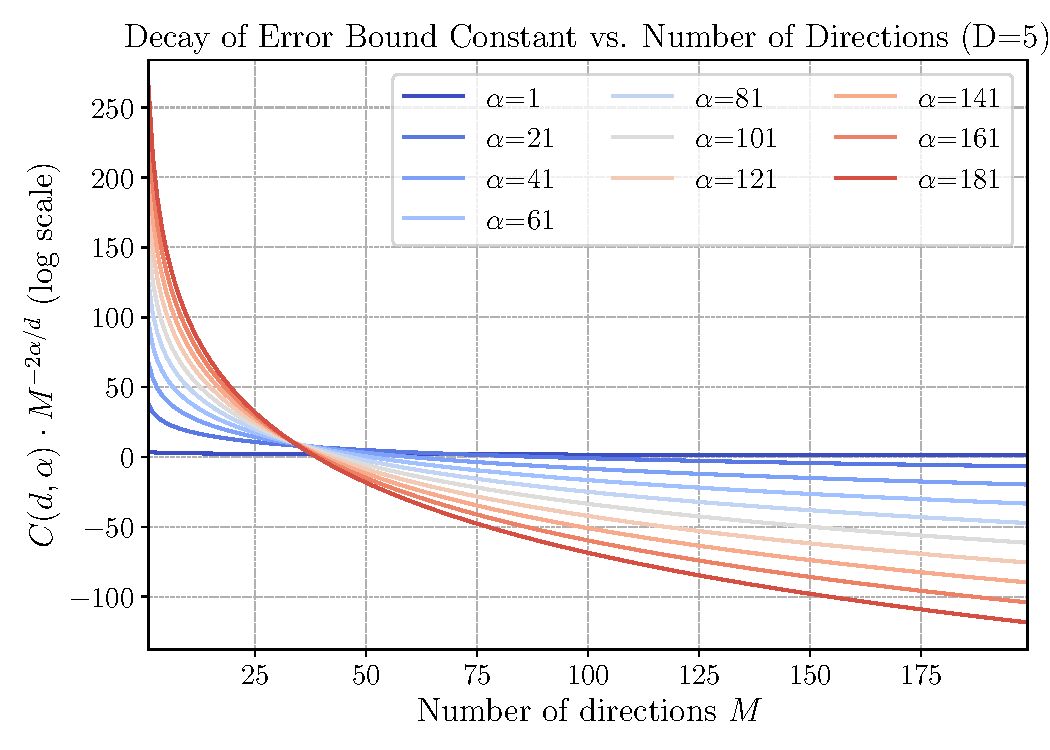
\includegraphics[width=0.49\linewidth]{toy_figures/bound_constant.pdf}
    \caption{\small Depiction of the expected BCS loss upper bound (\cref{thm:spherical_bounds}) for various smoothness values $\alpha$. We clearly see that as the smoothness increases ({\bf blue to red}), as the upper bound decreases more and more rapidly with $M$.}
    \label{fig:bound_example}
\end{figure*}



\begin{figure}[t!]
\centering
    \centering
    dimension=128, slices=10\\
    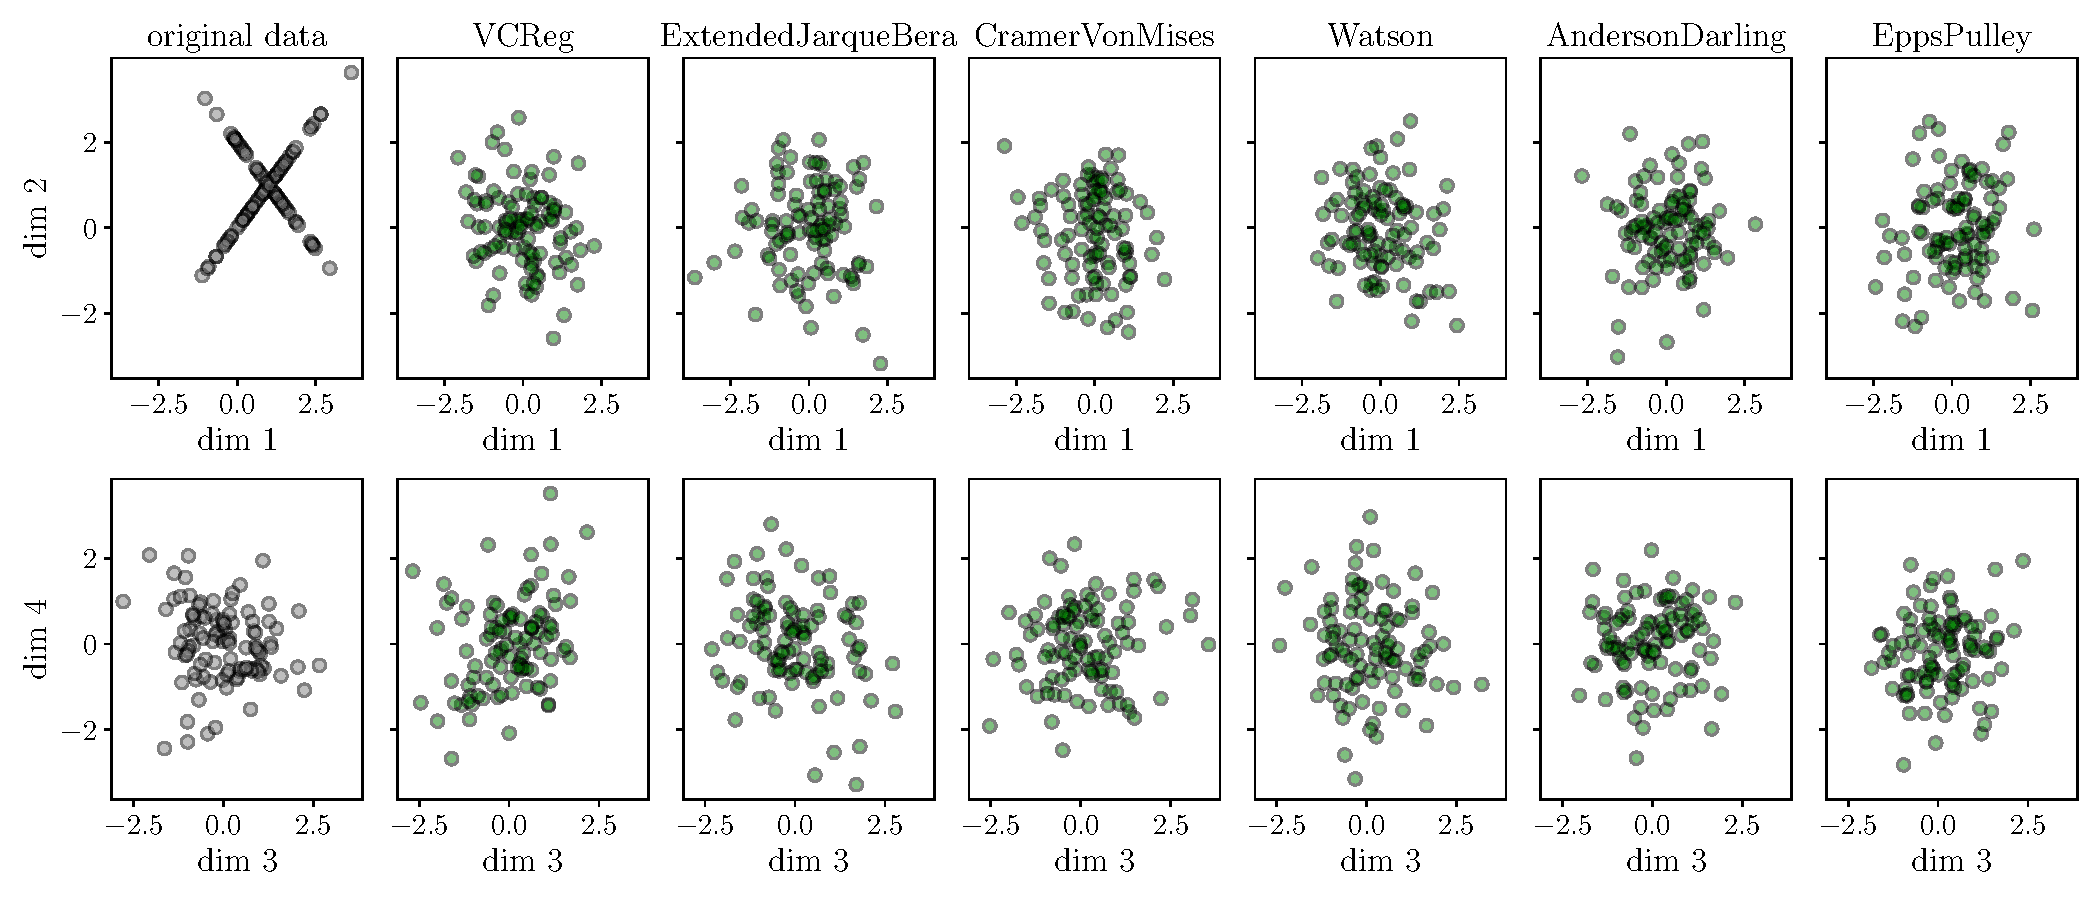
\includegraphics[width=0.9\linewidth]{toy_figures/nonparametric/2d_slicing_dim_128_N_100_slices_10.pdf}
    dimension=128, slices=100\\
    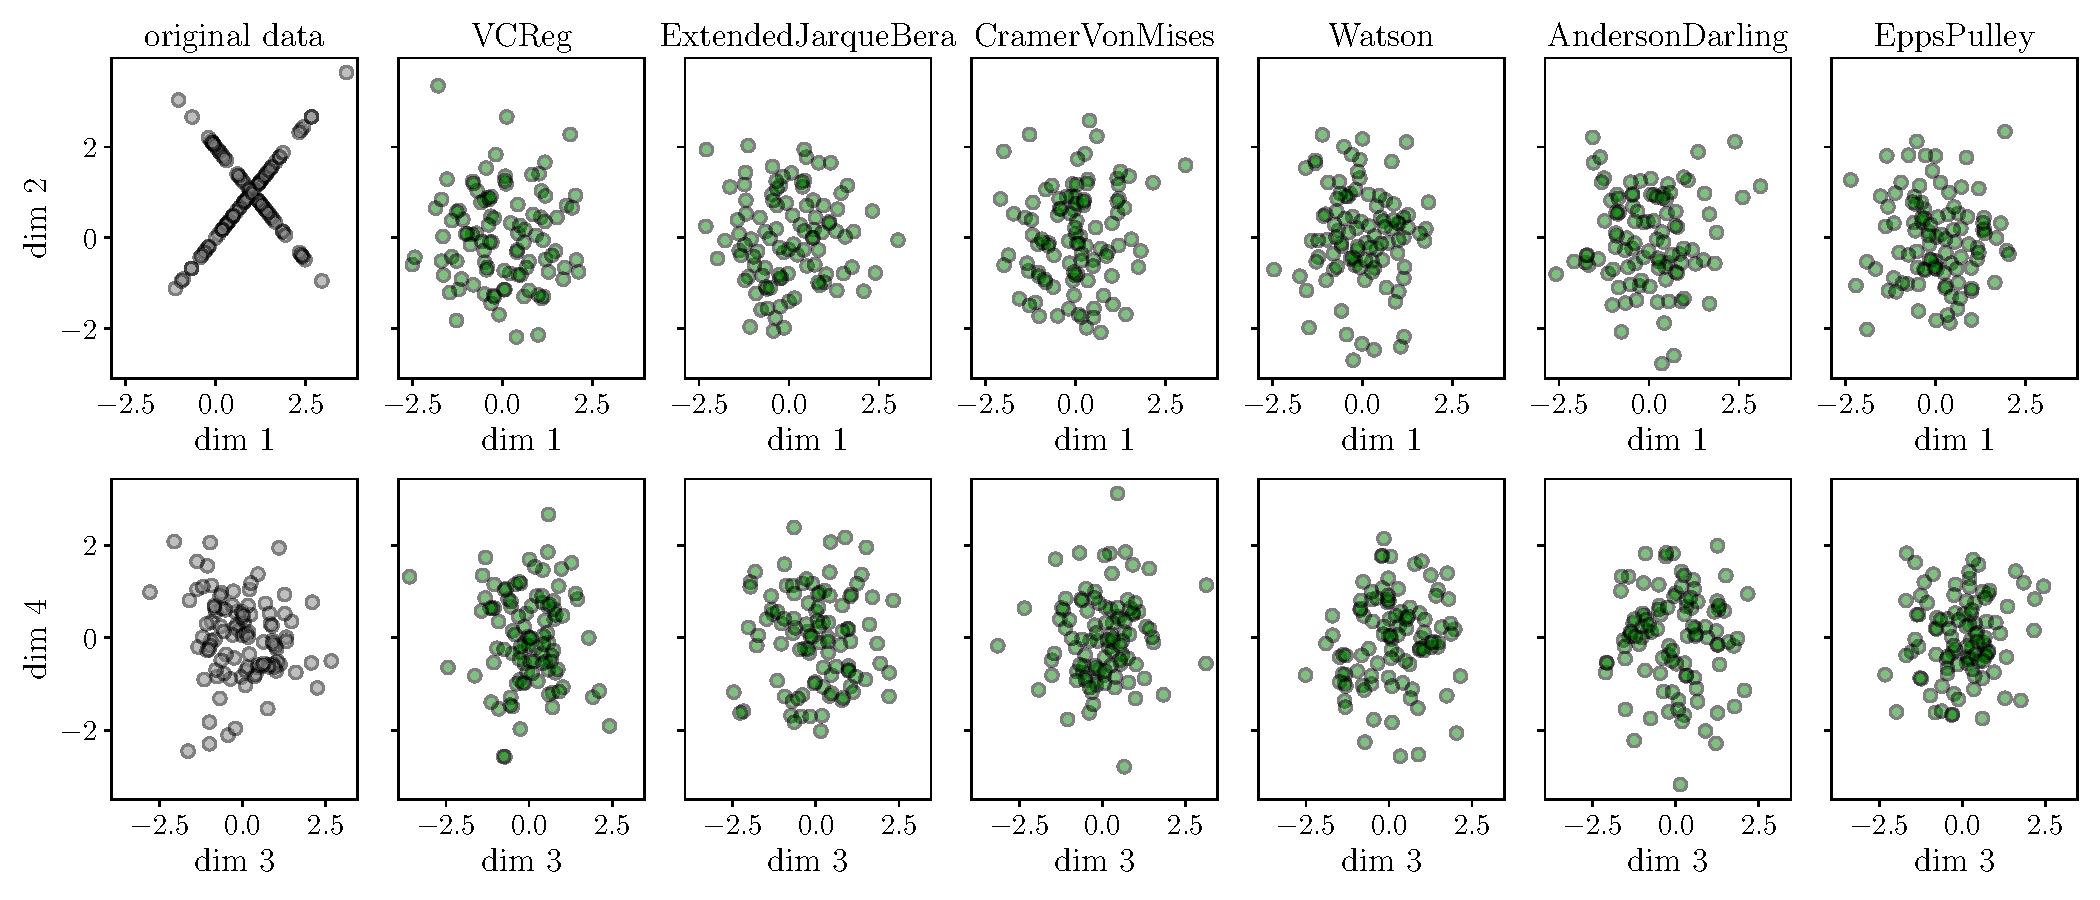
\includegraphics[width=0.9\linewidth]{toy_figures/nonparametric/2d_slicing_dim_128_N_100_slices_100.pdf}
    dimension=1024, slices=100\\
    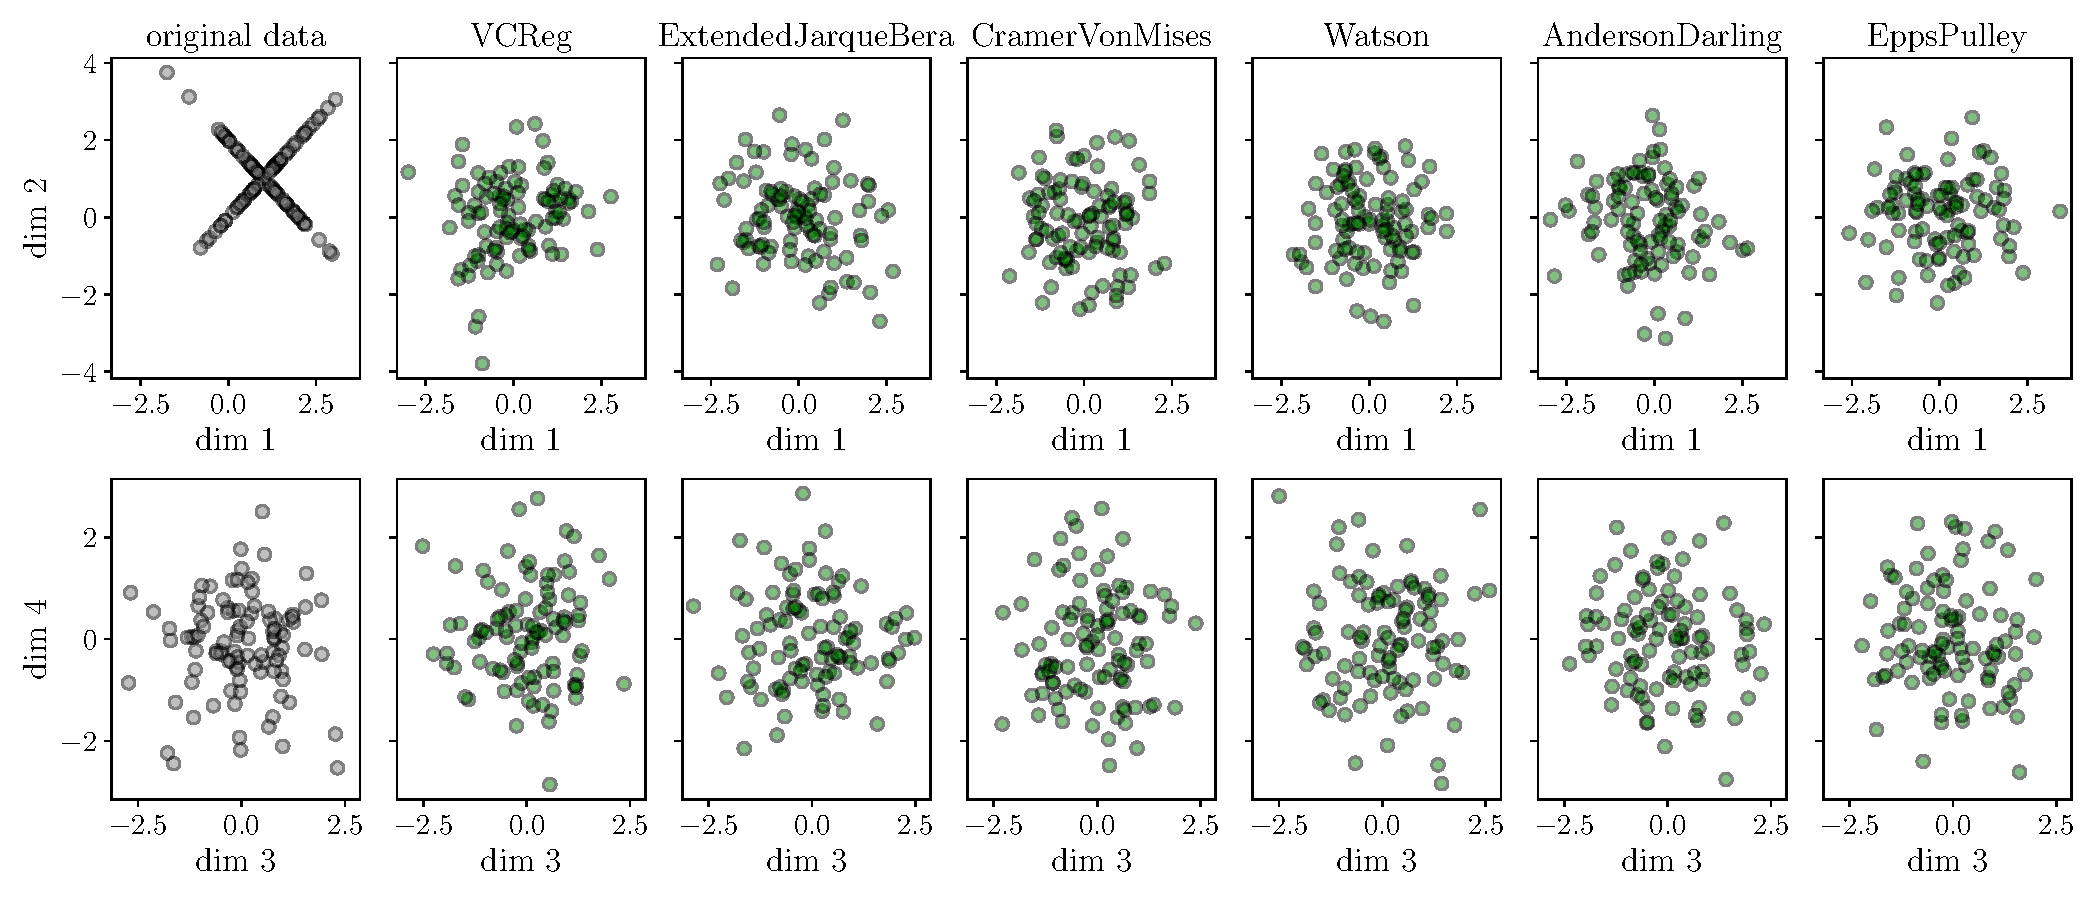
\includegraphics[width=0.9\linewidth]{toy_figures/nonparametric/2d_slicing_dim_1024_N_100_slices_100.pdf}
    \caption{Reprise of \cref{fig:nonparametric} for additional dimensions and number of 1d projections.}
    \label{fig:extra_nonparametric}
\end{figure}



\begin{figure}[t!]
    \centering
    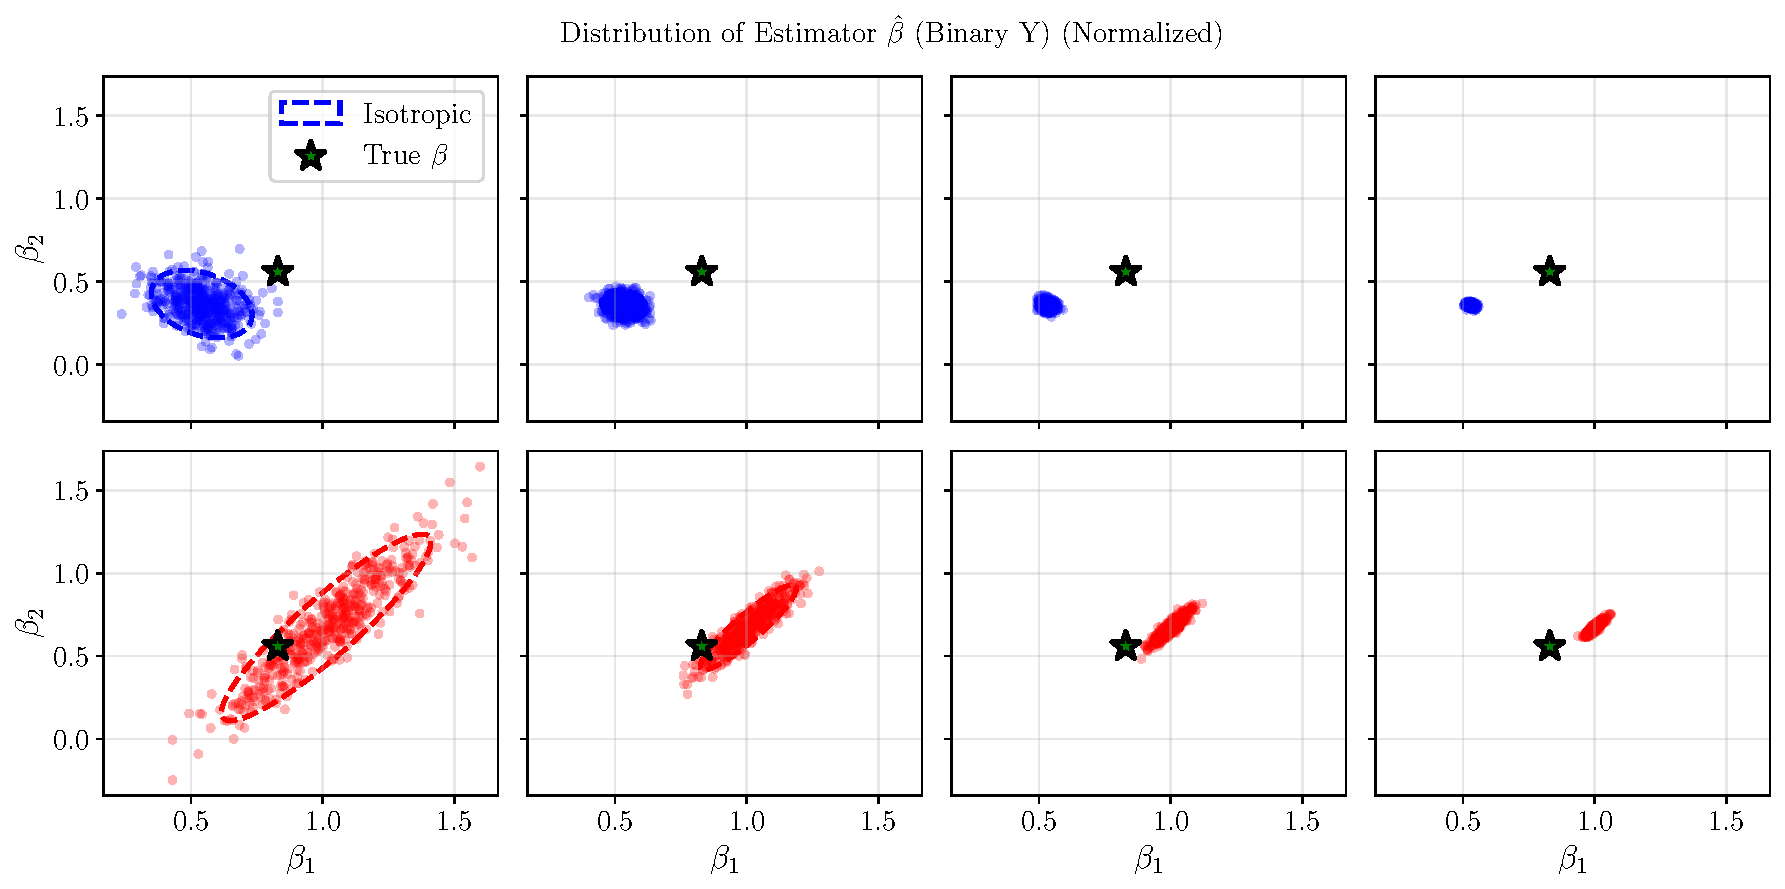
\includegraphics[width=0.8\linewidth]{toy_figures/le/beta_distributions_binary.pdf}
    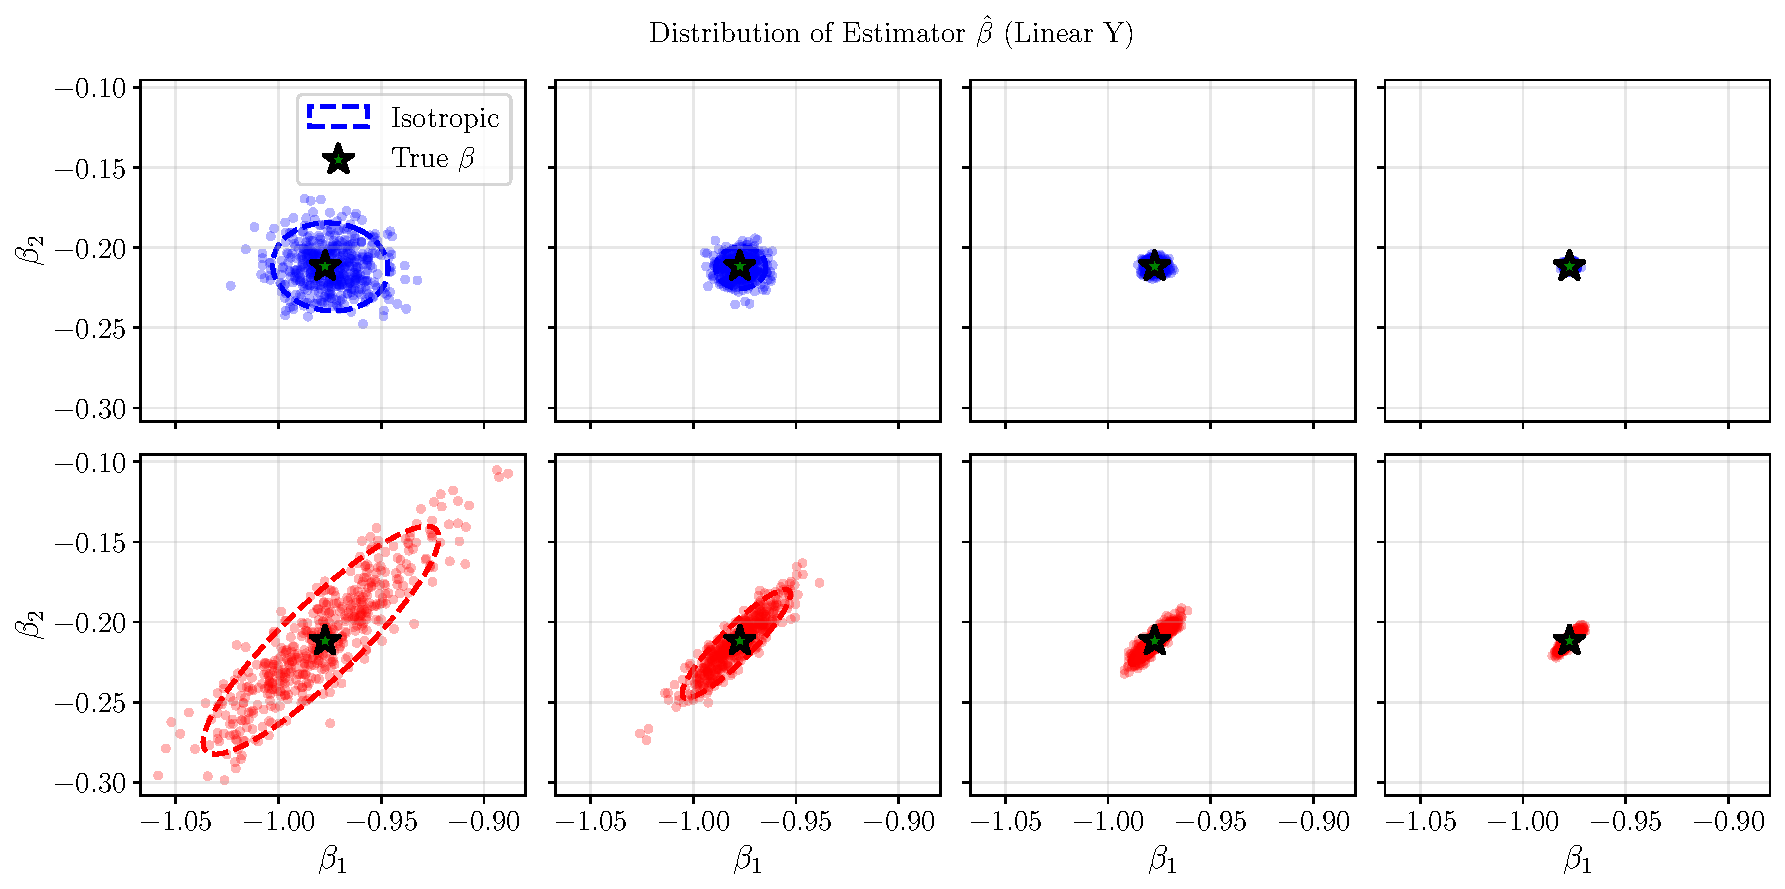
\includegraphics[width=0.8\linewidth]{toy_figures/le/beta_distributions_linear.pdf}
    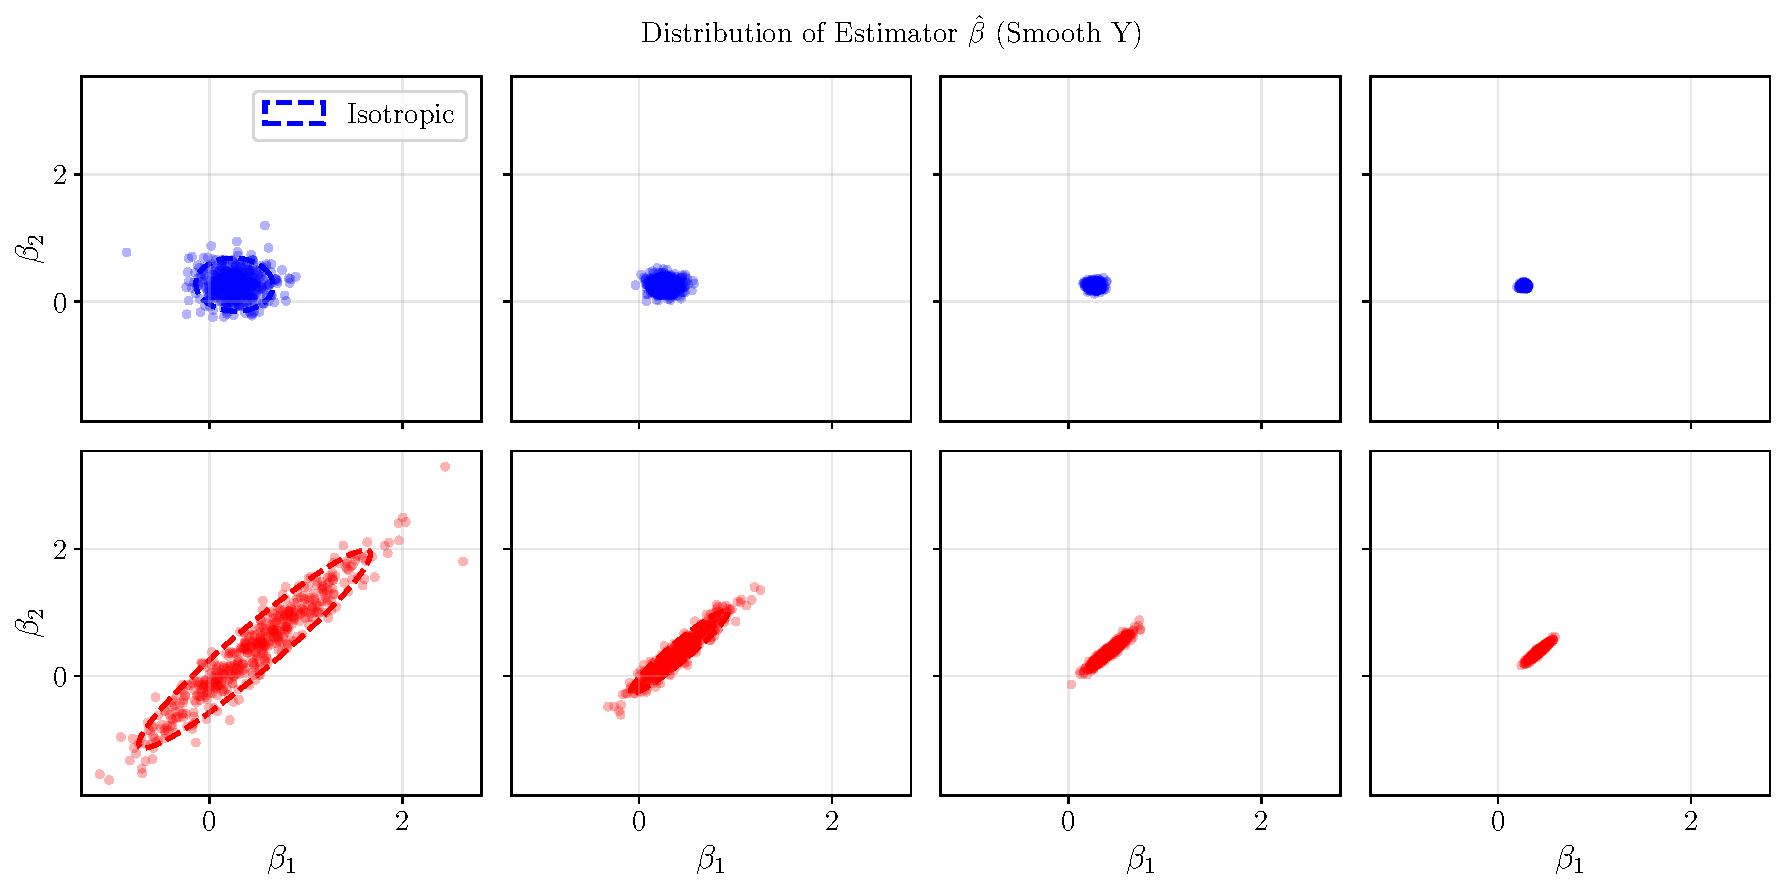
\includegraphics[width=0.8\linewidth]{toy_figures/le/beta_distributions_smooth.pdf}
    \caption{Depiction of the distribution of optimized $\beta$ values from OLS when comparing $\mZ_{\rm iso}$ and $\mZ_{\rm aniso}$ from \cref{thm:linear_probe_bias,thm:linear_probe_variance}. We clearly observe that the anisotropic version ({\bf blue}) provides much lower variance compared to the isotropic case ({\bf red}). We consider a binary classification (linear separable class) ({\bf top row}), a linear regression task ({\bf middle row}), and a nonlinear regression task with smooth targets ({\bf bottom row}). For each case, we resample the training samples numerous times and produce an estimate for $\beta$ each time. Because the data is $2$-dimensional, we can visualize the $\beta$ distribution directly.}
    \label{fig:beta_distributions}
\end{figure}


\begin{figure}
    \centering
    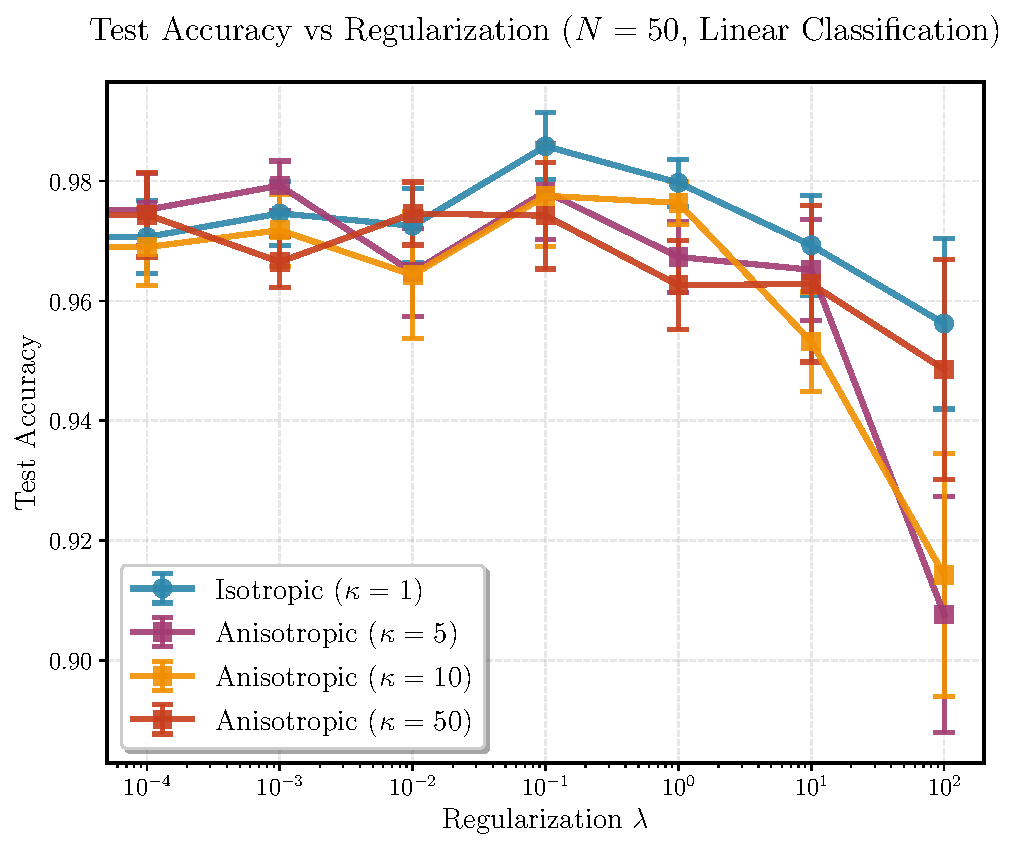
\includegraphics[width=0.32\linewidth]{toy_figures/le/acc_vs_lambda_N50_linear_classification.pdf}
    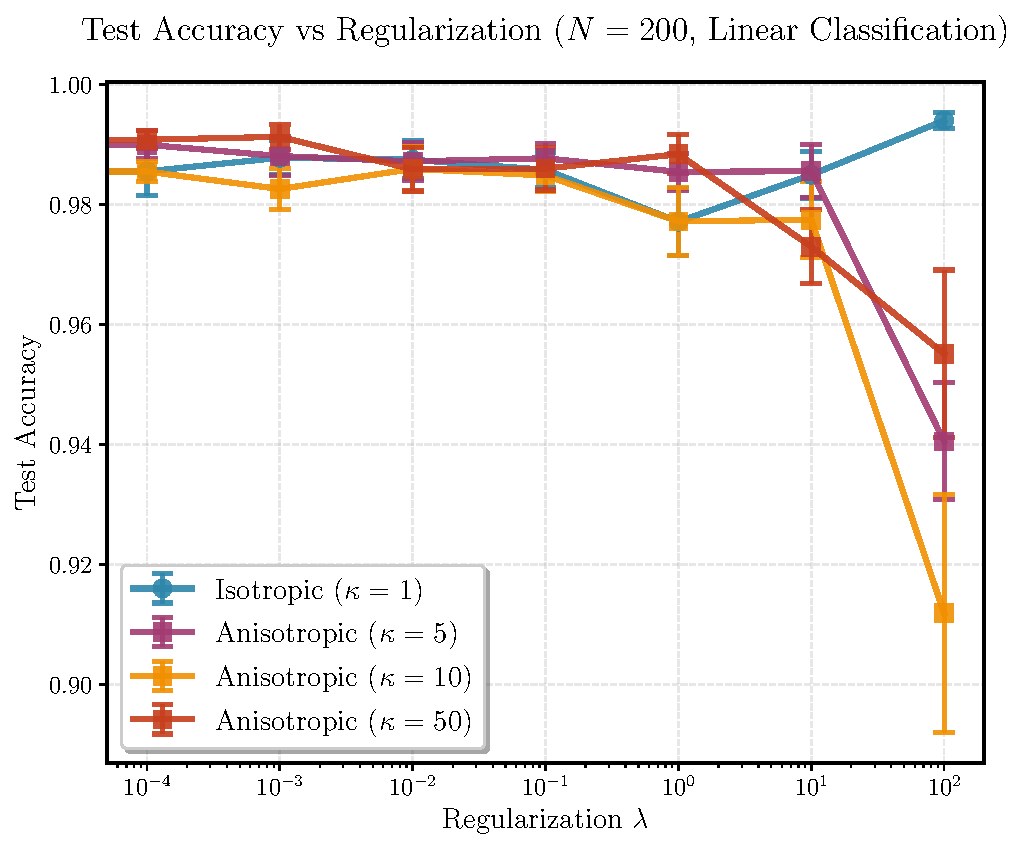
\includegraphics[width=0.32\linewidth]{toy_figures/le/acc_vs_lambda_N200_linear_classification.pdf}
    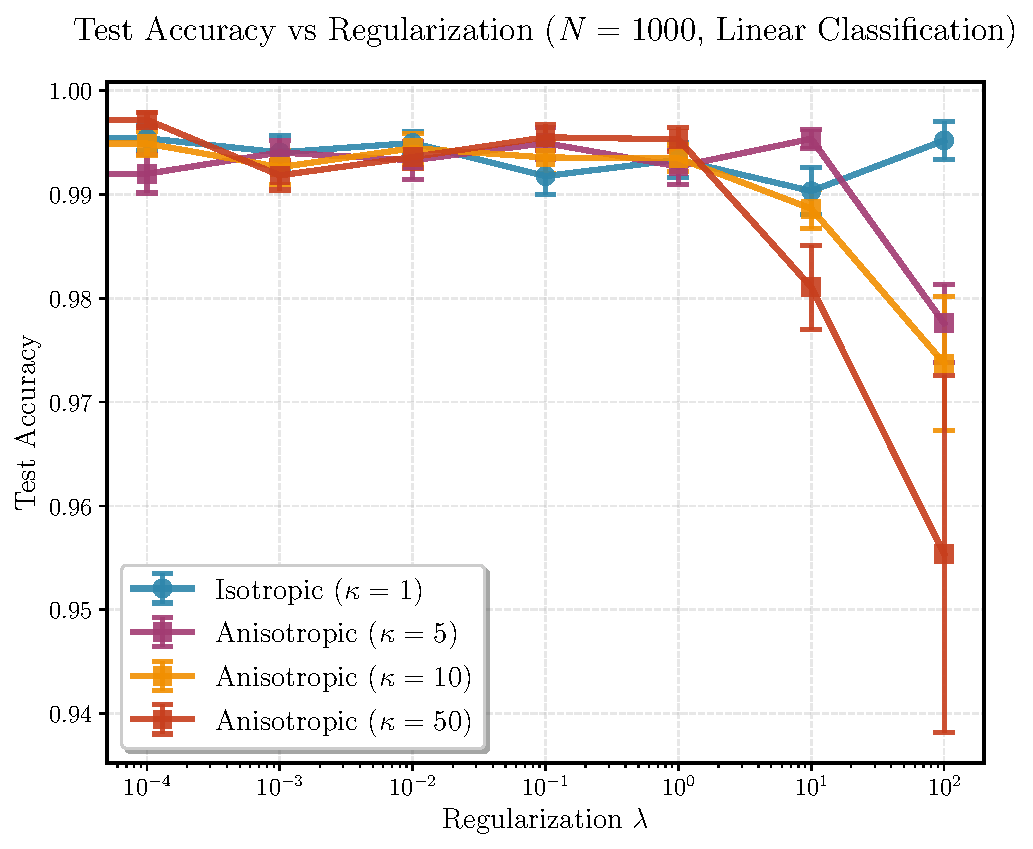
\includegraphics[width=0.32\linewidth]{toy_figures/le/acc_vs_lambda_N1000_linear_classification.pdf}\\
    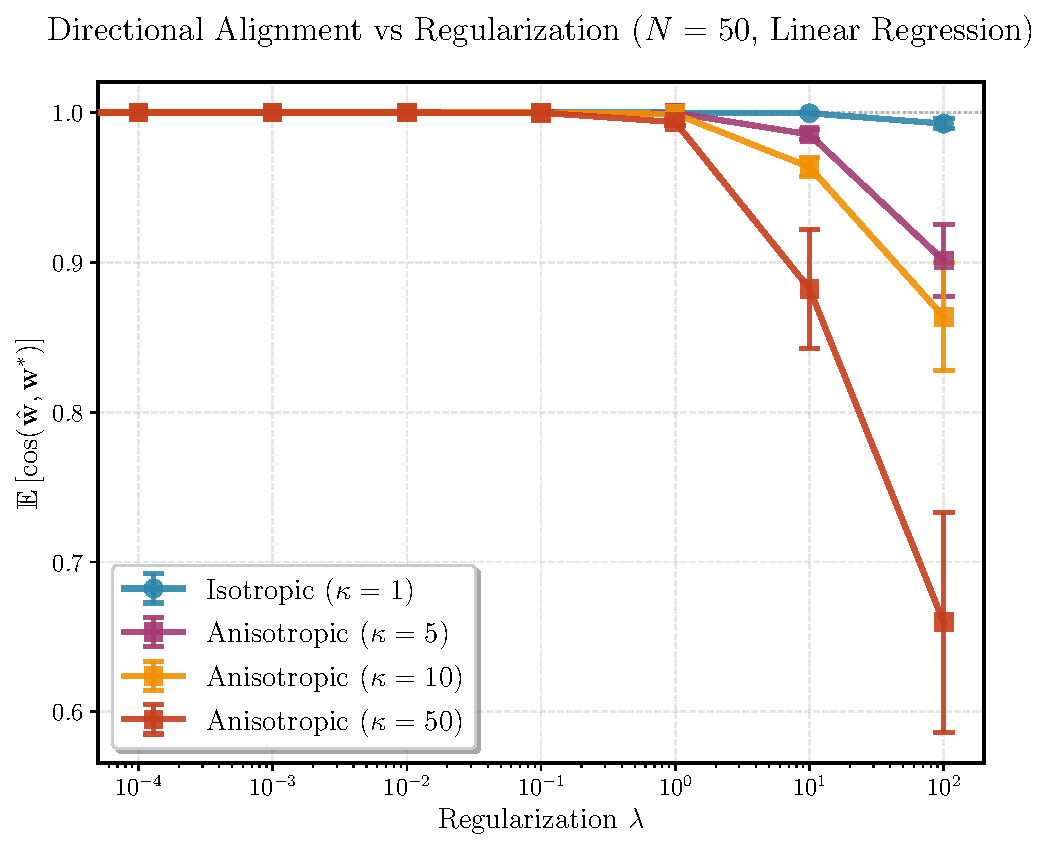
\includegraphics[width=0.32\linewidth]{toy_figures/le/cosine_vs_lambda_N50_linear_regression.pdf}
    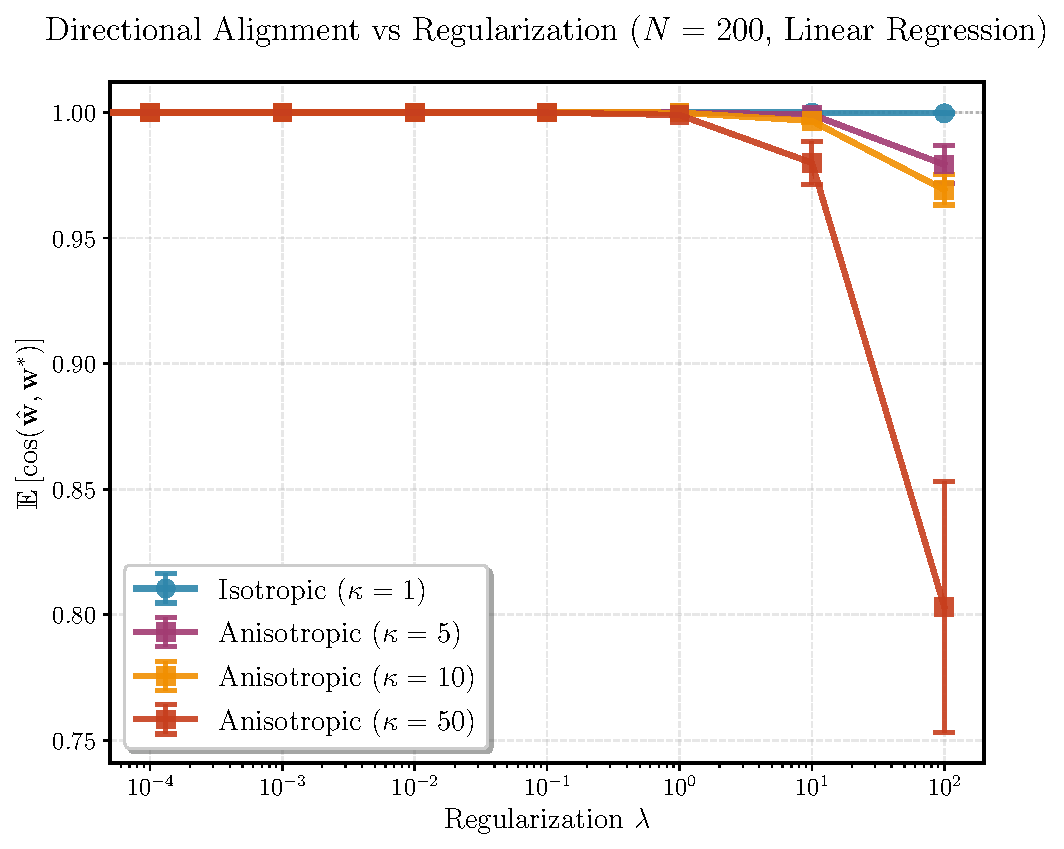
\includegraphics[width=0.32\linewidth]{toy_figures/le/cosine_vs_lambda_N200_linear_regression.pdf}
    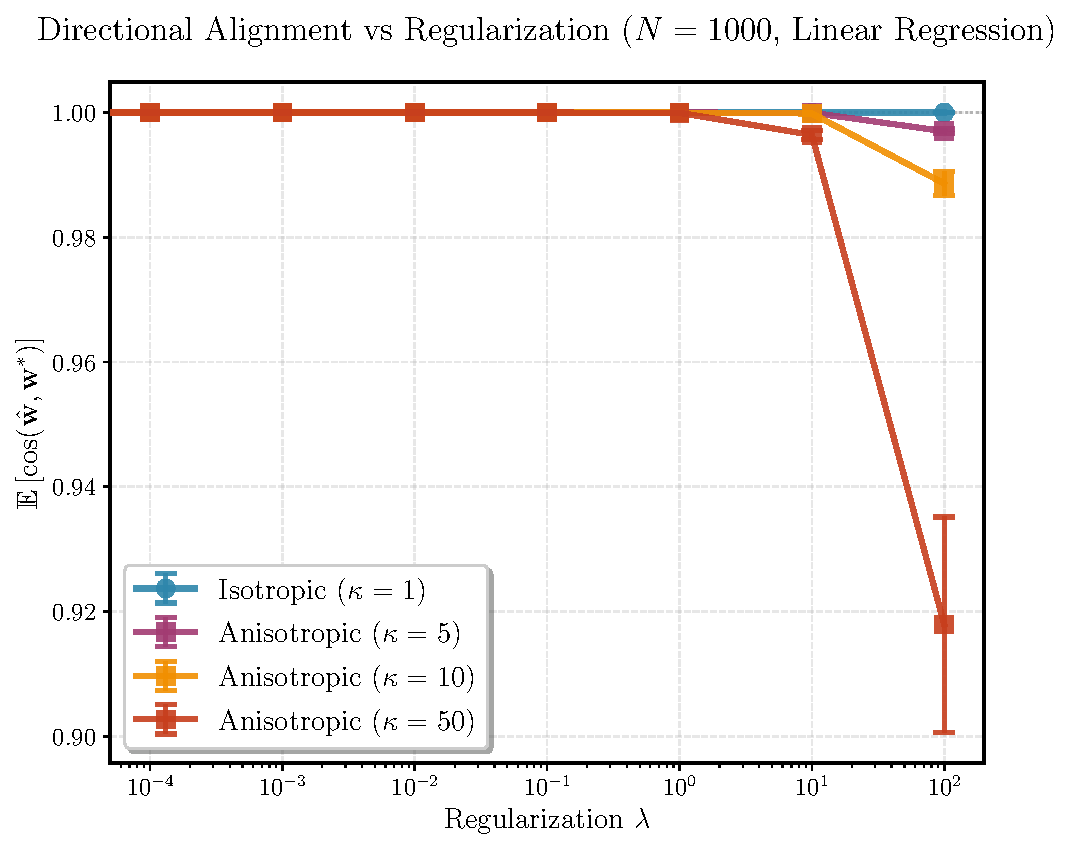
\includegraphics[width=0.32\linewidth]{toy_figures/le/cosine_vs_lambda_N1000_linear_regression.pdf}
    \caption{Depiction of accuracy ({\bf top}) and cosine similarity between estimated and true estimator ({\bf bottom}) for the OLS setting with varying strength of Tikhonov regularization ({\bf x-axis)} comparing isotropic and anisotropic embeddings. As per \cref{thm:gradient_bias}, the anisotropic distribution creates a bias in the OLS estimation for nonzero regularization.}
    \label{fig:ols_bias}
\end{figure}




\begin{figure}[t!]
    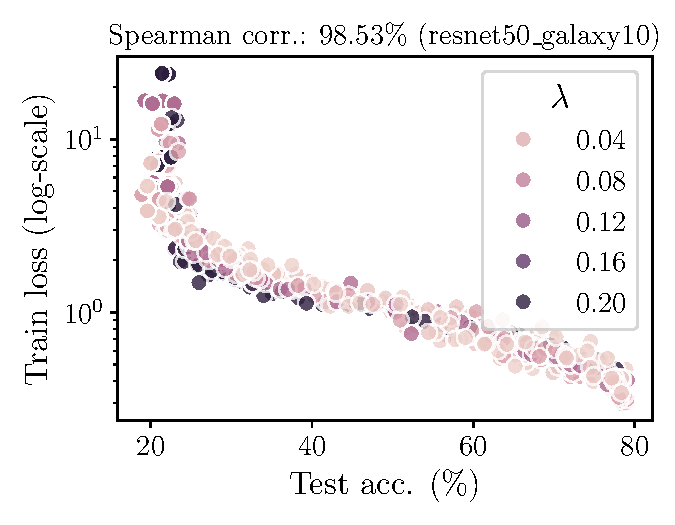
\includegraphics[width=0.33\linewidth]{toy_figures/exps/loss_corr/loss_corr_resnet50_galaxy10.pdf}
    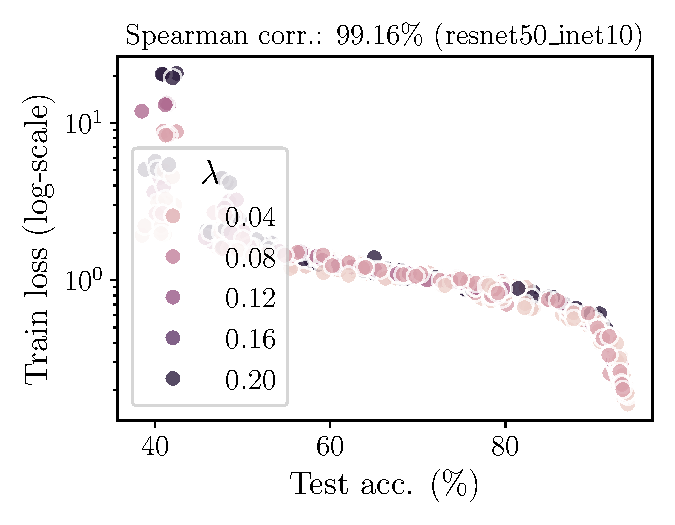
\includegraphics[width=0.33\linewidth]{toy_figures/exps/loss_corr/loss_corr_resnet50_inet10.pdf}
    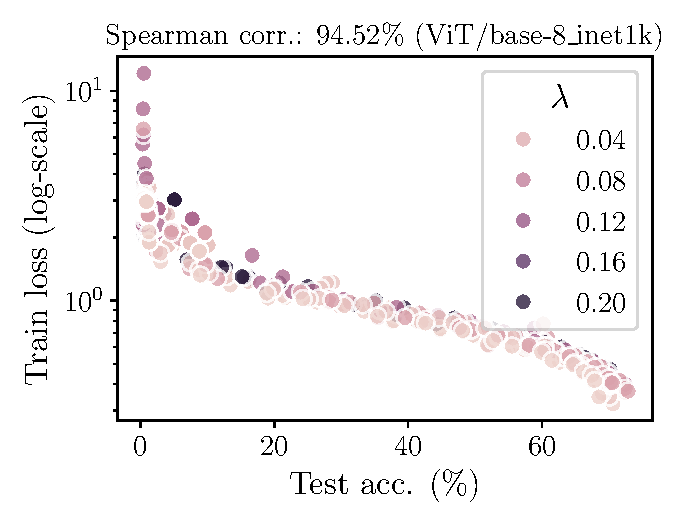
\includegraphics[width=0.33\linewidth]{toy_figures/exps/loss_corr/loss_corr_ViT-base-8_inet1k.pdf}
    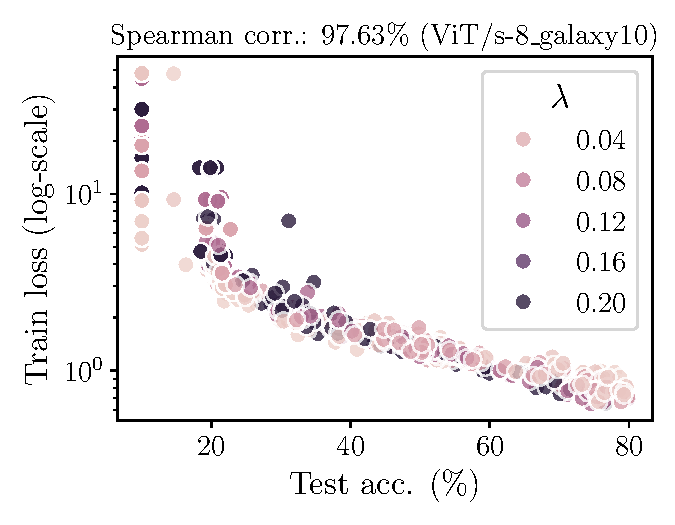
\includegraphics[width=0.33\linewidth]{toy_figures/exps/loss_corr/loss_corr_ViT-s-8_galaxy10.pdf}
    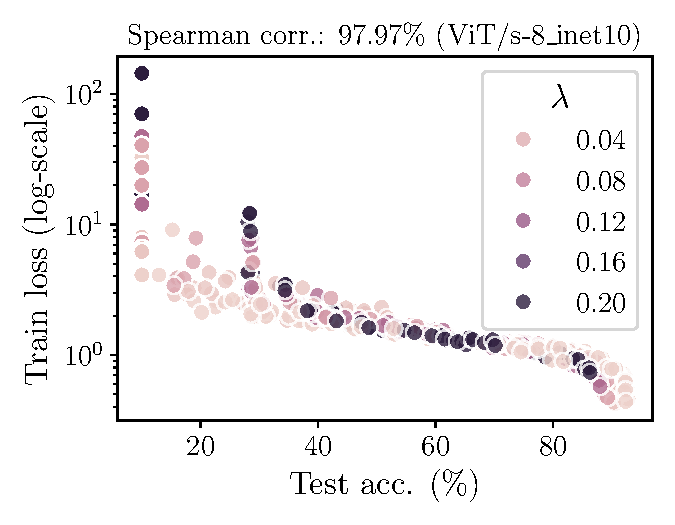
\includegraphics[width=0.33\linewidth]{toy_figures/exps/loss_corr/loss_corr_ViT-s-8_inet10.pdf}
    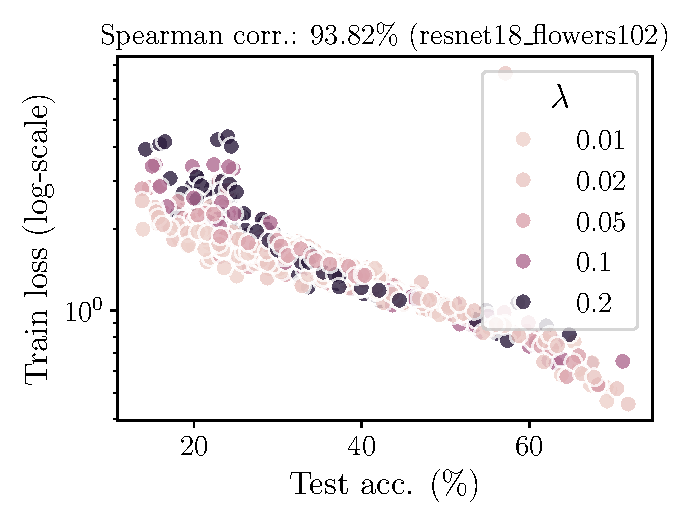
\includegraphics[width=0.33\linewidth]{toy_figures/exps/loss_corr/loss_corr_resnet18_flowers102.pdf}
    \caption{Additional figures provides in \cref{fig:corr_loss_extra}}
    \label{fig:corr_loss_extra}
\end{figure}



\begin{table}[t!]
\caption{Performance metrics across different sample sizes from \cref{fig:galaxy10}}
\label{tab:galaxy10}
\centering
\begin{tabular}{llrrrrrrr}
\toprule
\textbf{Freeze Backbone} & \textbf{Model Name} & \multicolumn{7}{c}{\textbf{Samples per Class}} \\
\cmidrule(lr){3-9}
 &  & \textbf{All} & \textbf{1} & \textbf{2} & \textbf{5} & \textbf{10} & \textbf{100} & \textbf{1000} \\
\midrule
\multirow[c]{6}{*}{\textbf{No}} 
 & \multicolumn{8}{l}{\textit{LeJEPA (Ours)}} \\
 & ConvNeXt-V2 Nano & 82.72 & \textbf{29.42} & \textbf{36.65} & \textbf{50.94} & \textbf{59.85} & \textbf{75.34} & 81.97 \\
 & LeViT-128 & 79.41 & 18.45 & 24.08 & 33.11 & 41.76 & 64.59 & 77.59 \\
 & ResNet-18 & 82.15 & 23.34 & 31.56 & 43.82 & 54.64 & 73.53 & 81.41 \\
 & ResNet-34 & \textbf{83.28} & 24.27 & 31.51 & 44.23 & 53.95 & 74.93 & \textbf{82.32} \\
\cmidrule(lr){2-9}
 & \multicolumn{8}{l}{\textit{Baselines}} \\
 & DINOv2 Small & 78.34 & 21.05 & 21.71 & 30.33 & 36.23 & 60.81 & 75.55 \\
 & DINOv3 ViT-S/16 & 81.60 & 24.71 & 29.43 & 37.71 & 44.71 & 69.87 & 80.54 \\
\midrule
\multirow[c]{6}{*}{\textbf{Yes}} 
 & \multicolumn{8}{l}{\textit{LeJEPA (Ours)}} \\
 & ConvNeXt-V2 Nano & 76.52 & 28.74 & 36.65 & 50.60 & 59.50 & 72.62 & 77.24 \\
 & LeViT-128 & 69.00 & 25.85 & 33.30 & 45.52 & 52.43 & 64.37 & 69.39 \\
 & ResNet-18 & 75.95 & 30.48 & 38.22 & 50.85 & 58.86 & 72.70 & 76.39 \\
 & ResNet-34 & \textbf{78.17} & \textbf{31.08} & \textbf{38.33} & \textbf{52.26} & \textbf{60.63} & \textbf{74.77} & \textbf{78.62} \\
\cmidrule(lr){2-9}
 & \multicolumn{8}{l}{\textit{Baselines}} \\
 & DINOv2 Small & 67.62 & 27.68 & 32.22 & 40.72 & 47.72 & 62.49 & 67.89 \\
 & DINOv3 ViT-S/16 & 71.38 & 30.17 & 36.65 & 45.74 & 51.51 & 65.90 & 71.35 \\
\bottomrule
\end{tabular}
\end{table}






\begin{figure}
    \centering
    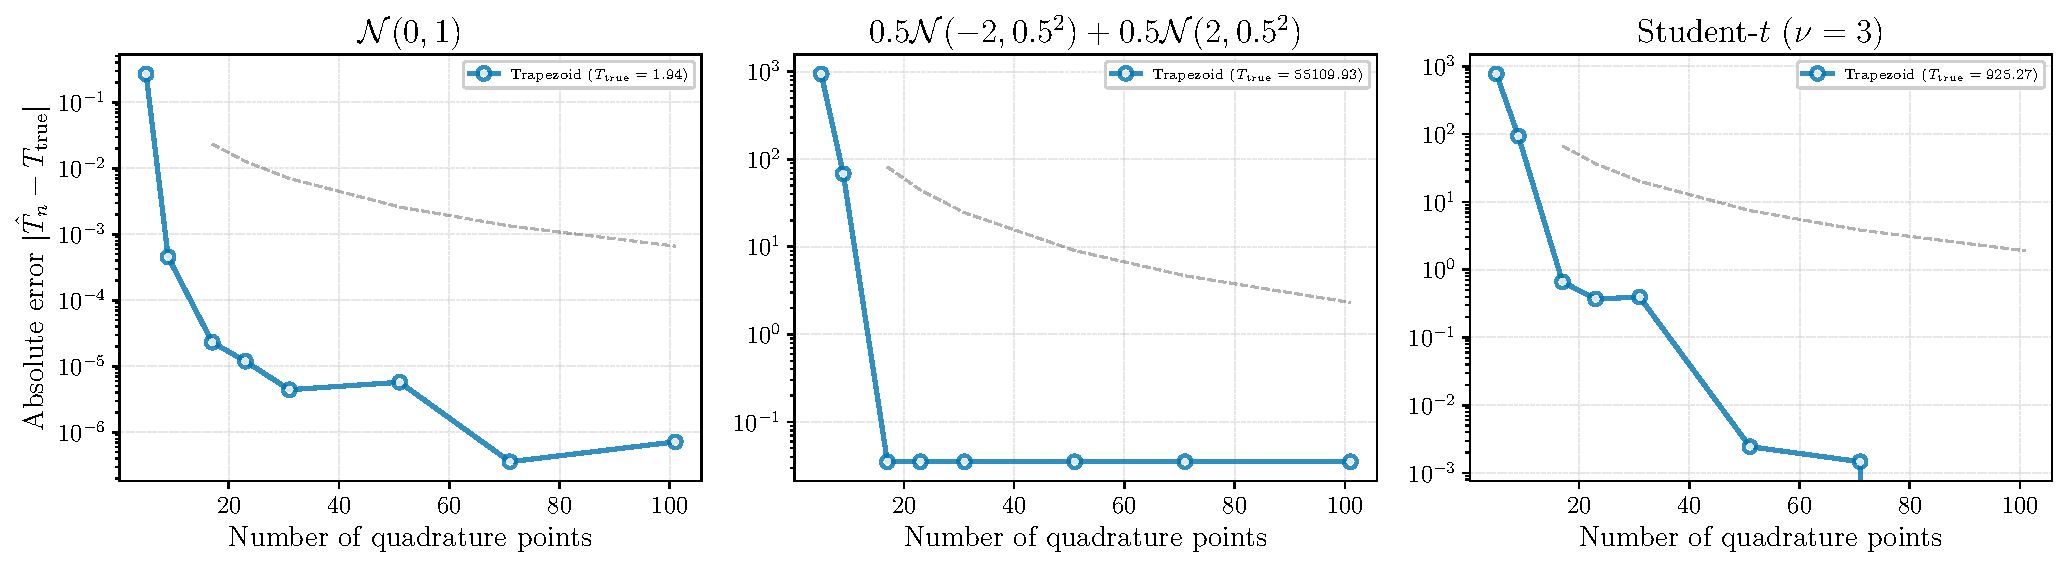
\includegraphics[width=\linewidth]{toy_figures/quadrature_convergence.pdf}
    \caption{Proposed trapezoid quadrature for the Epps-Pulley statistic as implemented in \cref{lst:epps-pulley-pytorch}. We depict the approximation error of the integral for various distributions, demonstrate rapid convergence (faster than quadratic show in {\bf grey line}) across possible embedding distributions.}
    \label{fig:quadrature}
\end{figure}


\begin{figure*}[t!]
    
    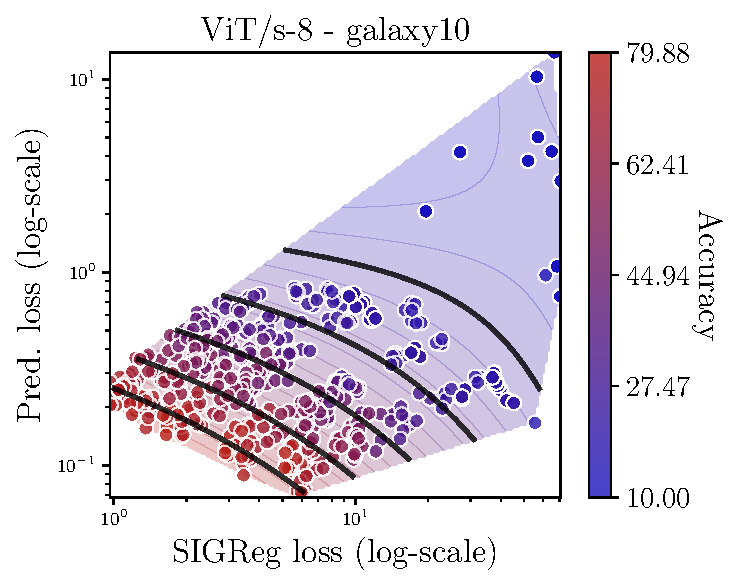
\includegraphics[width=0.33\linewidth]{toy_figures/exps/loss_corr/selection_ViT-s-8_galaxy10.pdf}
    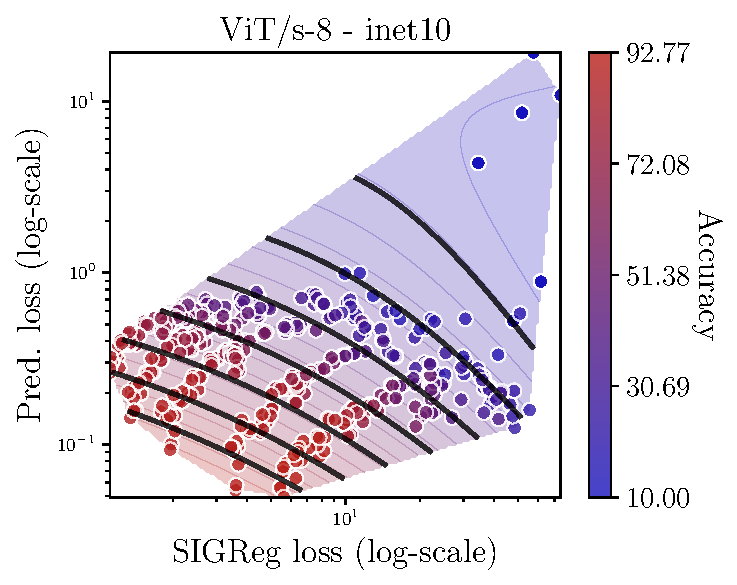
\includegraphics[width=0.33\linewidth]{toy_figures/exps/loss_corr/selection_ViT-s-8_inet10.pdf}
    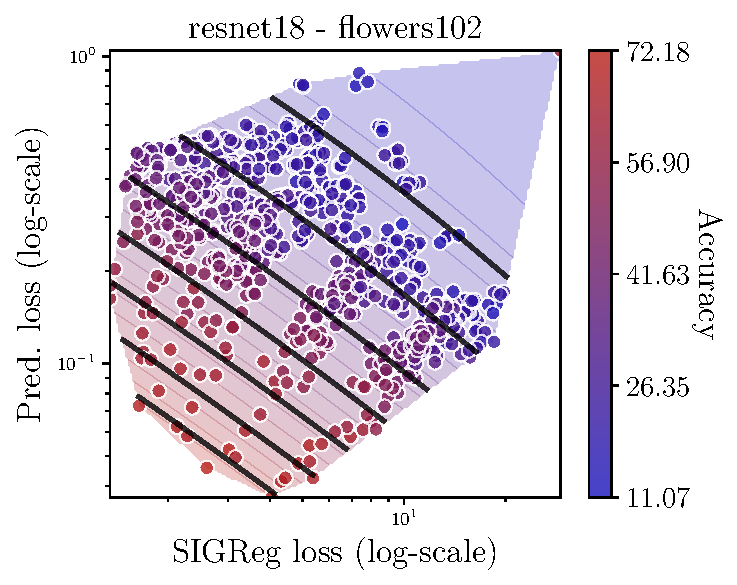
\includegraphics[width=0.33\linewidth]{toy_figures/exps/loss_corr/selection_resnet18_flowers102.pdf}
    \caption{Additional figures for \cref{fig:heatmap_loss}.}
    \label{fig:extra_heatmap_loss}
\end{figure*}



\begin{table*}[t!]
\caption{Top 1 accuracy (in \%) with LeJEPA pretraining on Imagenet-100 for 400 epochs (All values are percentages)}
\label{tab:proj_pred}
\begin{tabular}{ll|lll|lll|lll}
\toprule
 & backbone & \multicolumn{3}{c}{resnet50} & \multicolumn{3}{c}{vit\_small\_patch8\_224} & \multicolumn{3}{c}{vit\_tiny\_patch8\_224} \\
 & Projector & 1-layer & 2-layer & 3-layer & 1-layer & 2-layer & 3-layer & 1-layer & 2-layer & 3-layer \\
w/ predictor & w/ SWA &  &  &  &  &  &  &  &  &  \\
\midrule
\multirow[c]{2}{*}{False} & False & 79.71 & 82.44 & 83.93 & 76.59 & 80.77 & 81.07 & 71.79 & 76.87 & 80.37 \\
 & True & 79.79 & 82.69 & 83.50 & 79.96 & 83.63 & 84.12 & 75.86 & 82.36 & 80.50 \\
\multirow[c]{2}{*}{True} & False & 79.41 & 82.44 & 83.57 & 77.58 & 79.41 & 81.91 & 67.74 & 77.64 & 80.73 \\
 & True & 78.87 & 82.04 & 82.82 & 77.11 & 81.77 & 82.58 & 69.53 & 78.27 & 79.77 \\
\bottomrule
\end{tabular}
\end{table*}



\begin{table*}[t!]
\caption{{\bf Small architecture in-domain LeJEPA pretraining} from random initialization across datasets and architectures, with frozen backbone linear evaluation. First, {\bf LeJEPA is able to produce near state-of-the-art performances on tiny dataset with only a thousand samples}, e.g., flowers102. Second, {\bf on non-natural image data, LeJEPA clearly outperforms the latest frontier vision models}, e.g., Galaxy10. See \cref{fig:galaxy10} for additional experiments with varying number of training samples and with full finetuning.}
\label{tab:in_domain}
\begin{tabular}{llllllll}
\toprule
 & Pretraining & flowers102 & cifar100 & food101 & inet10 & cifar10 & galaxy10 \\
 & \# train. samples & 1020 & 50000 & 75750 & 13000 & 50000 & 11008 \\
\midrule
LeJEPA (convnextv2\_nano) 14M & in-domain & 64.34 & 69.26 & 69.59 & 90.81 & 92.22 & 76.05 \\
LeJEPA (resnet18) 11M & in-domain & 74.57 & 69.94 & 73.57 & 92.36 & 92.51 & 75.32 \\
LeJEPA (resnet34) 21M & in-domain & 71.85 & 70.44 & 74.95 & 92.80 & 93.16 & 77.29 \\
LeJEPA (resnext26ts) 8M & in-domain & 82.19 & 69.10 & 76.77 & 92.82 & 91.59 & 73.78 \\
LeJEPA (swin\_tiny) 27M & in-domain & 63.94 & 65.08 & 78.40 & 92.87 & 92.67 & 74.89 \\
IJEPA-inet22k (ViT-H/14) 630M & inet1k & 85.76 & 86.93 & 81.06 & 98.65 & 97.77 & 62.93
\end{tabular}
\end{table*}



\begin{table}[t!]
    \centering
    \setlength{\tabcolsep}{0.5em}
    \caption{Time (in millisecond) to compute the proposed SIGReg loss from \cref{lst:epps-pulley-pytorch} on a Tesla V100-SXM2-16GB for varying mini-batch size ($N$), number of slices ($M$), integration points. Results are computed over $10$ runs.}
    \label{tab:times}
    \begin{tabular}{rrrrr}
\toprule
N & M & \makecell{\# integration \\ points} & mean (ms) & std (ms) \\
\midrule
 512 & 512 &  16 & 0.465236 & 0.011642 \\
 512 & 512 &  64 & 0.461317 & 0.003894 \\
 512 & 512 &  256 & 0.627644 & 0.003337 \\
 2048 & 512 &  16 & 1.406441 & 0.002415 \\
 8192 & 512 &  16 & 6.188304 & 0.007226 \\
 8192 & 8192 &  16 & 8.685009 & 0.038829 \\
 32768 & 512 &  16 & 26.373118 & 0.012732 \\
 512 & 2048 &  16 & 0.465614 & 0.005274 \\
 512 & 8192 &  16 & 0.670379 & 0.006854 \\
\bottomrule
\end{tabular}
\end{table}


\begin{table}[t!]
\caption{Number of \cref{fig:lambda_views}.}
\label{tab:lambda_perf}
\begin{tabular}{lllllllllllll}
\toprule
 & \multicolumn{12}{c}{resnet50} \\
$\lambda$ & 0.001 & 0.005 & 0.010 & 0.020 & 0.025 & 0.050 & 0.100 & 0.150 & 0.200 & 0.300 & 0.400 & 0.500 \\
\#views &  &  &  &  &  &  &  &  &  &  &  &  \\
\midrule
2 & 81.41 & 82.73 & 83.49 & 82.99 & 82.23 & - & - & - & - & - & - & - \\
4 & 79.88 & 83.04 & 84.36 & 84.68 & 84.33 & 83.00 & 82.91 & 81.05 & 78.58 & - & - & - \\
8 & 76.67 & 81.58 & 83.59 & 83.49 & 83.76 & 84.32 & 83.66 & 83.07 & 82.16 & 81.00 & 79.25 & 77.72  \\
\bottomrule
\end{tabular}
\end{table}



\section{Details on Low-Discrepancy Sequences}
\label{sec:low_discrepancy}

Quasi-Monte Carlo (QMC) methods, such as the Sobol sequence, are widely used to generate low-discrepancy samples in the unit hypercube, providing improved uniformity over purely random sampling. To obtain samples uniformly distributed on the hypersphere, each QMC point is mapped to a standard normal vector via the inverse cumulative distribution function (CDF), and then projected onto the sphere by normalization. This approach leverages the rotational invariance of the multivariate normal distribution, ensuring that the resulting directions are uniformly distributed on the sphere's surface. While the low-discrepancy property is not strictly preserved under this nonlinear mapping, the resulting samples are empirically more uniform than random samples and are standard in high-dimensional applications \cite{marsaglia1972choosing,dick2010digital,caflisch1998monte}.
% \begin{algorithm}[H]
% \caption{Quasi-Monte Carlo Sampling on the $d$-Dimensional Unit Hypersphere}
% \label{alg:qmc_hypersphere}
\begin{algorithmic}[1]
\Require Number of points $N$, dimension $d$
\Ensure Points $\{\mathbf{y}_i\}_{i=1}^N$ quasi-uniformly distributed on $\mathbb{S}^{d-1}$
\For{$i = 1$ to $N$}
    \State Generate $\mathbf{x}_i \in [0,1]^d$ as the $i$-th point of a Sobol sequence
    \State Transform each component: $z_{i,j} = \Phi^{-1}(x_{i,j})$ for $j = 1, \ldots, d$ \Comment{$\Phi^{-1}$ is the inverse CDF of the standard normal}
    \State Normalize: $\mathbf{y}_i = \mathbf{z}_i / \|\mathbf{z}_i\|_2$
\EndFor
\end{algorithmic}
% \end{algorithm}









\section{Shapiro-Wilk Test}
\label{sec:shapiro_wilk}

Let X1 < X2 < . . . < Xn denote an ordered random sample of size n from a standard normal distribution. Also, let m 5 (m1,m2,...,mn) be the vector of expected values of standard normal order statistics, and let V 5 (vij ) be the corresponding n 3 n covariance matrix, so that
\begin{equation}
    E\left(X_{i}\right)=m_{i} \quad \text { and } \quad \operatorname{cov}\left(X_{i}, X_{j}\right)=v_{i j}, \quad i, j=1,2, \ldots, n
\end{equation}
The W test statistic \cite{shapiro1965analysis} for normality is then denoted by
\begin{equation}
    \begin{array}{l}
W=\frac{\left(\sum_{i=1}^{n} a_{i} Y_{i}\right)}{\sum_{i=1}^{n}\left(Y_{i} -\bar{Y}\right)^{2}}=\frac{(\mathbf{a} \mathbf{Y})}{S^{2}}\\
\mathbf{a}^{\prime}=\left(a_{1}, a_{2}, \ldots, a_{n}\right)=\mathbf{m} \mathbf{V}^{-1}\left(\mathbf{m} \mathbf{V}^{-1} \mathbf{V}^{-1} \mathbf{m}\right)^{-1 / 2}\\
\mathrm{S}^{2}=\sum_{i=1}^{n}\left(Y_{i}-\bar{Y}\right)^{2}
\end{array}
\end{equation}

\cite{shapiro1972approximate} suggested replacing the covariance matrix V by the identity matrix I, because for large samples, the observations {Yi} may be treated as if they are independent (see \cite{gupta1952estimation}). Another asymptotic extension was suggested by \cite{weisburg1975approximate}
\begin{equation}
    E\left(X_{i}\right)=m_{i} \approx\Phi^{-1}\left(\frac{i-\frac{3}{8}}{n+\frac{1}{4}}\right) \quad i=1,2, \ldots, n
\end{equation}
building atop \cite{elfving1947asymptotical}'s approximation but using $3/8$ instead of $\pi/8$.

\cite{rahman1997modification} proposed another variation using the approximation for the expected values of order statistics given by \cite{blom1958statistical} and the approximations for the elements of the variance± covariance matrix given by \cite{blom1958statistical,mosteller2006some}. These approximations are
\begin{equation}
    E\left(X_{i}\right)=m_{i} \approx \Phi^{-1}\left(\frac{i}{N+1}\right), \quad i=1,2, \ldots, n
\end{equation}
\begin{equation}
    \operatorname{cov}\left(X_{i}, X_{j}\right)=v_{i j} \approx \frac{p_{i} p_{j}}{(n+2) f\left(m_{i}\right) f\left(m_{j}\right)}, \quad i, j=1,2, \ldots, n
\end{equation}
\begin{equation}
    p_{i}=\frac{i}{n+1}
\end{equation}



We know (see \cite{hammersley1954estimation,plackett1958linear})
\begin{equation}
    \begin{array}{l}
\mathbf{V}^{-1}=(n+1)(n+2) \\
\times\left(\begin{array}{cccccc}
2 \phi^{2}\left(m_{1}\right) & -\phi\left(m_{1}\right) \phi\left(m_{2}\right) & 0 & 0 & \ldots & 0 \\
-\phi\left(m_{1}\right) \phi\left(m_{2}\right) & 2 \phi^{2}\left(m_{2}\right) & -\phi\left(m_{2}\right) \phi\left(m_{3}\right) & 0 & \ldots & 0 \\
0 & -\phi\left(m_{2}\right) \phi\left(m_{3}\right) & 2 \phi^{2}\left(m_{3}\right) & -\phi\left(m_{3}\right) \phi\left(m_{4}\right) & \ldots & 0 \\
\vdots & & & & & \\
0 & 0 & 0 & 0 & \ldots & 2 \phi^{2}\left(m_{n}\right)
\end{array}\right)
\end{array}
\end{equation}




\section{Multivariate Statistics}
\label{sec:multivariate_tests}


% The entire goal of most SSL methods is to produce
% \begin{align*}
%     f(\vx) \sim \mathcal{N}(\mathbf{0},\mI),
% \end{align*}
% under the argument that this is the maximum Entropy distribution hereby preserving as much information about the input as possible. Note that the Gaussian with covariance $\mSigma$ is the density that has maximum entropy amongst all densities with covariance $\mSigma$. The choice of $\mSigma = \mI$ in particular may feel more arbitrary and convenient. There is an argument on having an isotropic covariance matrix as those are the ones occupying move volume (TBD).

% Note that the von Mises–Fisher distribution is the one of maximum Entropy when the circular moment and circular Covariance is specified\footnote{\url{https://arxiv.org/pdf/2010.10918}}. It is obtained from an isotropic Gaussian conditioned on normalized samples. That may be a benefit of isotropic Covariance.


We ideally would like to compare the distributions. One slight variation is to compare the Characteristic function of the distributions. Given samples $\vx_1,\dots,\vx_N$, the Empirical Characteristic Function (ECF) is defined as 
\begin{align*}
    \hat{\psi}_{N}(\vt) = \frac{1}{N}\sum_{n=1}^{N} e^{-i \vt^\top \vy_n}.
\end{align*}
We can now compare our ECF to the one of the target distribution and build the statistic
\begin{align*}
    N\int |\hat{\psi}_{N}(\vt) - \psi_{0}(\vt) |^2\omega(\vt) dt=N\int |\hat{\psi}_{N}(\vt) - e^{-\|\vt\|_2/2} |^2\omega(\vt) dt,
\end{align*}
if the weighting function is given by $\omega(\vt) = (2\pi \beta ^2 )^{-d/2}e^{-\frac{\|\vt\|_2^2}{2}}$ then the following simplification can be made
\begin{align*}
\mathrm{BHEP}_{n, \beta}= & \frac{1}{n} \sum_{j, k=1}^{n} \exp \left(-\frac{\beta^{2}\left\|Y_{n, j}-Y_{n, k}\right\|^{2}}{2}\right) \\
& -\frac{2}{\left(1+\beta^{2}\right)^{d / 2}} \sum_{j=1}^{n} \exp \left(-\frac{\beta^{2}\left\|Y_{n, j}\right\|^{2}}{2\left(1+\beta^{2}\right)}\right)+\frac{n}{\left(1+2 \beta^{2}\right)^{d / 2}} .
\end{align*}
with $\beta>0$, Baringhaus-Henze-Epps-Pulley. From \footnote{\url{https://www.routledge.com/Density-Estimation-for-Statistics-and-Data-Analysis/Silverman/p/book/9780412246203?srsltid=AfmBOoodlL-CtlqL0JVC-LcP6mOWw6VTt51_YstdZOW4W3iuicu1VFyg}}
leading to the HZ test \footnote{\url{https://www.tandfonline.com/doi/abs/10.1080/03610929008830400}} uses
\begin{equation}
    \beta_{n}=2^{-1 / 2}((2 d+1) n / 4)^{1 /(d+4)}
\end{equation}




the same can be done with the moment generating function \footnote{\url{https://arxiv.org/pdf/1711.07199}}
\begin{align*}
T_{n, \beta}=\pi^{d / 2}\left(\frac{1}{n} \sum_{i, j=1}^{n} \frac{1}{\beta^{d / 2}} \exp \left(\frac{\left\|Y_{n, i}+Y_{n, j}\right\|^{2}}{4 \beta}\right)+\frac{n}{(\beta-1)^{d / 2}}\right. \\
\left.-2 \sum_{j=1}^{n} \frac{1}{(\beta-1 / 2)^{d / 2}} \exp \left(\frac{\left\|Y_{n, j}\right\|^{2}}{4 \beta-2}\right)\right),
\end{align*}
here with $\beta>2$

There is also one combining both\footnote{\url{https://arxiv.org/pdf/1706.03029}}!
\begin{equation}
    \begin{array}{l}
T_{n, \gamma}:=\int_{\mathbb{R}^{d}} U_{n}^{2}(t) w_{\gamma}(t) \mathrm{d} t\\
U_{n}(t):=\sqrt{n}\left(R_{n}(t) M_{n}(t)-1\right)
\end{array}
\end{equation}
\begin{equation}
    \begin{aligned}
T_{n, \gamma}= & \left(\frac{\pi}{\gamma}\right)^{d / 2}\left\{\frac { 1 } { 2 n ^ { 3 } } \sum _ { j , k , l , m = 1 } ^ { n } \left[\exp \left(\frac{\left\|Y_{j k}^{+}\right\|^{2}-\left\|Y_{\ell m}^{-}\right\|^{2}}{4 \gamma}\right) \cos \left(\frac{Y_{j k}^{+\top} Y_{\ell m}^{-}}{2 \gamma}\right)\right.\right. \\
+ & \left.\exp \left(\frac{\left\|Y_{j k}^{+}\right\|^{2}-\left\|Y_{\ell m}^{+}\right\|^{2}}{4 \gamma}\right) \cos \left(\frac{Y_{j k}^{+\top} Y_{\ell m}^{+}}{2 \gamma}\right)\right] \\
& \left.-\frac{2}{n} \sum_{j, k=1}^{n} \exp \left(\frac{\left\|Y_{n, j}\right\|^{2}-\left\|Y_{n, k}\right\|^{2}}{4 \gamma}\right) \cos \left(\frac{Y_{n, j}^{\top} Y_{n, k}}{2 \gamma}\right)+n\right\},
\end{aligned}
\end{equation}
and its simplified version
\begin{equation}
    \widetilde{T}_{n, \gamma}:=\int_{\mathbb{R}^{d}} U_{n}(t) w_{\gamma}(t) \mathrm{d} t .
\end{equation}
\begin{equation}
    \widetilde{T}_{n, \gamma}=\left(\frac{\pi}{\gamma}\right)^{d / 2} \sqrt{n}\left(\frac{1}{n^{2}} \sum_{j, k=1}^{n} \exp \left(\frac{\left\|Y_{n, j}\right\|^{2}-\left\|Y_{n, k}\right\|^{2}}{4 \gamma}\right) \cos \left(\frac{Y_{n, j}^{\top} Y_{n, k}}{2 \gamma}\right)-1\right)
\end{equation}


Also one testing the derivative \footnote{\url{https://arxiv.org/pdf/1901.03986}}

\begin{equation}
    \mathrm{HV}_{n, \gamma}:=n \int\left\|\nabla M_{n}(t)-t M_{n}(t)\right\|^{2} \widetilde{w}_{\gamma}(t) \mathrm{d} t
\end{equation}
\begin{equation}\mathrm{HV}_{n, \gamma}=\frac{1}{n}\left(\frac{\pi}{\gamma}\right)^{d / 2} \sum_{j, k=1}^{n} \exp \left(\frac{\left\|Y_{n, j, k}^{+}\right\|^{2}}{4 \gamma}\right)
\left(Y_{n, j}^{\top} Y_{n, k}-\frac{\left\|Y_{n, j, k}^{+}\right\|^{2}}{2 \gamma}+\frac{d}{2 \gamma}+\frac{\left\|Y_{n, j, k}^{+}\right\|^{2}}{4 \gamma^{2}}\right) .
\end{equation}


skewness
\footnote{\url{https://www.jstor.org/stable/2334770}}:
\begin{equation}
    b_{1, d}=\frac{1}{n^{2}} \sum_{j, k=1}^{n}\left(Y_{n, j}^{\top} Y_{n, k}\right)^{3}
\end{equation}
skewness
\footnote{\url{https://link.springer.com/article/10.1007/s13171-020-00211-6}}:
\begin{equation}
    \widetilde{b}_{1, d}=\frac{1}{n^{2}} \sum_{j, k=1}^{n} Y_{n, j}^{\top} Y_{n, k}\left\|Y_{n, j}\right\|^{2}\left\|Y_{n, k}\right\|^{2}
\end{equation}
which should be 0 for Gaussian and Kurtosis which should be d(d+2)
\begin{equation}
    b_{2, d}=\frac{1}{n} \sum_{j=1}^{n}\left\|Y_{n, j}\right\|^{4}
\end{equation}


